\documentclass[twoside]{book}

% Packages required by doxygen
\usepackage{fixltx2e}
\usepackage{calc}
\usepackage{doxygen}
\usepackage[export]{adjustbox} % also loads graphicx
\usepackage{graphicx}
\usepackage[utf8]{inputenc}
\usepackage{makeidx}
\usepackage{multicol}
\usepackage{multirow}
\PassOptionsToPackage{warn}{textcomp}
\usepackage{textcomp}
\usepackage[nointegrals]{wasysym}
\usepackage[table]{xcolor}

% Font selection
\usepackage[T1]{fontenc}
\usepackage[scaled=.90]{helvet}
\usepackage{courier}
\usepackage{amssymb}
\usepackage{sectsty}
\renewcommand{\familydefault}{\sfdefault}
\allsectionsfont{%
  \fontseries{bc}\selectfont%
  \color{darkgray}%
}
\renewcommand{\DoxyLabelFont}{%
  \fontseries{bc}\selectfont%
  \color{darkgray}%
}
\newcommand{\+}{\discretionary{\mbox{\scriptsize$\hookleftarrow$}}{}{}}

% Page & text layout
\usepackage{geometry}
\geometry{%
  a4paper,%
  top=2.5cm,%
  bottom=2.5cm,%
  left=2.5cm,%
  right=2.5cm%
}
\tolerance=750
\hfuzz=15pt
\hbadness=750
\setlength{\emergencystretch}{15pt}
\setlength{\parindent}{0cm}
\setlength{\parskip}{3ex plus 2ex minus 2ex}
\makeatletter
\renewcommand{\paragraph}{%
  \@startsection{paragraph}{4}{0ex}{-1.0ex}{1.0ex}{%
    \normalfont\normalsize\bfseries\SS@parafont%
  }%
}
\renewcommand{\subparagraph}{%
  \@startsection{subparagraph}{5}{0ex}{-1.0ex}{1.0ex}{%
    \normalfont\normalsize\bfseries\SS@subparafont%
  }%
}
\makeatother

% Headers & footers
\usepackage{fancyhdr}
\pagestyle{fancyplain}
\fancyhead[LE]{\fancyplain{}{\bfseries\thepage}}
\fancyhead[CE]{\fancyplain{}{}}
\fancyhead[RE]{\fancyplain{}{\bfseries\leftmark}}
\fancyhead[LO]{\fancyplain{}{\bfseries\rightmark}}
\fancyhead[CO]{\fancyplain{}{}}
\fancyhead[RO]{\fancyplain{}{\bfseries\thepage}}
\fancyfoot[LE]{\fancyplain{}{}}
\fancyfoot[CE]{\fancyplain{}{}}
\fancyfoot[RE]{\fancyplain{}{\bfseries\scriptsize Generated by Doxygen }}
\fancyfoot[LO]{\fancyplain{}{\bfseries\scriptsize Generated by Doxygen }}
\fancyfoot[CO]{\fancyplain{}{}}
\fancyfoot[RO]{\fancyplain{}{}}
\renewcommand{\footrulewidth}{0.4pt}
\renewcommand{\chaptermark}[1]{%
  \markboth{#1}{}%
}
\renewcommand{\sectionmark}[1]{%
  \markright{\thesection\ #1}%
}

% Indices & bibliography
\usepackage{natbib}
\usepackage[titles]{tocloft}
\setcounter{tocdepth}{3}
\setcounter{secnumdepth}{5}
\makeindex

% Hyperlinks (required, but should be loaded last)
\usepackage{ifpdf}
\ifpdf
  \usepackage[pdftex,pagebackref=true]{hyperref}
\else
  \usepackage[ps2pdf,pagebackref=true]{hyperref}
\fi
\hypersetup{%
  colorlinks=true,%
  linkcolor=blue,%
  citecolor=blue,%
  unicode%
}

% Custom commands
\newcommand{\clearemptydoublepage}{%
  \newpage{\pagestyle{empty}\cleardoublepage}%
}

\usepackage{caption}
\captionsetup{labelsep=space,justification=centering,font={bf},singlelinecheck=off,skip=4pt,position=top}

%===== C O N T E N T S =====

\begin{document}

% Titlepage & ToC
\hypersetup{pageanchor=false,
             bookmarksnumbered=true,
             pdfencoding=unicode
            }
\pagenumbering{alph}
\begin{titlepage}
\vspace*{7cm}
\begin{center}%
{\Large J\+J\+MS }\\
\vspace*{1cm}
{\large Generated by Doxygen 1.8.14}\\
\end{center}
\end{titlepage}
\clearemptydoublepage
\pagenumbering{roman}
\tableofcontents
\clearemptydoublepage
\pagenumbering{arabic}
\hypersetup{pageanchor=true}

%--- Begin generated contents ---
\chapter{J\+J\+MS}
\label{index}\hypertarget{index}{}J\+J\+MS is a software system designed for a logistic company with the same name. This company provides a 24/7 customized delivery service that is supported by the system in question. Customers can request deliveries via an application on their phones or a web interface. Workers use the application on their phones to register deliveries and be assigned their next job.

Project developed in the context of the Software Engineering course at {\bfseries Universidade do Minho}. 
\chapter{Namespace Index}
\section{Namespace List}
Here is a list of all documented namespaces with brief descriptions\+:\begin{DoxyCompactList}
\item\contentsline{section}{\mbox{\hyperlink{namespacemvc_j_j_m_s}{mvc\+J\+J\+MS}} }{\pageref{namespacemvc_j_j_m_s}}{}
\item\contentsline{section}{\mbox{\hyperlink{namespacemvc_j_j_m_s_1_1_controllers}{mvc\+J\+J\+M\+S.\+Controllers}} }{\pageref{namespacemvc_j_j_m_s_1_1_controllers}}{}
\item\contentsline{section}{\mbox{\hyperlink{namespacemvc_j_j_m_s_1_1_data}{mvc\+J\+J\+M\+S.\+Data}} }{\pageref{namespacemvc_j_j_m_s_1_1_data}}{}
\item\contentsline{section}{\mbox{\hyperlink{namespacemvc_j_j_m_s_1_1_models}{mvc\+J\+J\+M\+S.\+Models}} }{\pageref{namespacemvc_j_j_m_s_1_1_models}}{}
\end{DoxyCompactList}

\chapter{Hierarchical Index}
\section{Class Hierarchy}
This inheritance list is sorted roughly, but not completely, alphabetically\+:\begin{DoxyCompactList}
\item \contentsline{section}{mvc\+J\+J\+M\+S.\+Models.\+Cartao\+Credito}{\pageref{classmvc_j_j_m_s_1_1_models_1_1_cartao_credito}}{}
\item Controller\begin{DoxyCompactList}
\item \contentsline{section}{mvc\+J\+J\+M\+S.\+Controllers.\+Cartao\+Controller}{\pageref{classmvc_j_j_m_s_1_1_controllers_1_1_cartao_controller}}{}
\item \contentsline{section}{mvc\+J\+J\+M\+S.\+Controllers.\+Cliente\+Controller}{\pageref{classmvc_j_j_m_s_1_1_controllers_1_1_cliente_controller}}{}
\item \contentsline{section}{mvc\+J\+J\+M\+S.\+Controllers.\+Encomenda\+Controller}{\pageref{classmvc_j_j_m_s_1_1_controllers_1_1_encomenda_controller}}{}
\item \contentsline{section}{mvc\+J\+J\+M\+S.\+Controllers.\+Fornecedor\+Controller}{\pageref{classmvc_j_j_m_s_1_1_controllers_1_1_fornecedor_controller}}{}
\item \contentsline{section}{mvc\+J\+J\+M\+S.\+Controllers.\+Funcionario\+Controller}{\pageref{classmvc_j_j_m_s_1_1_controllers_1_1_funcionario_controller}}{}
\item \contentsline{section}{mvc\+J\+J\+M\+S.\+Controllers.\+Menu\+Cliente\+Controller}{\pageref{classmvc_j_j_m_s_1_1_controllers_1_1_menu_cliente_controller}}{}
\item \contentsline{section}{mvc\+J\+J\+M\+S.\+Controllers.\+Menu\+Funcionario\+Controller}{\pageref{classmvc_j_j_m_s_1_1_controllers_1_1_menu_funcionario_controller}}{}
\item \contentsline{section}{mvc\+J\+J\+M\+S.\+Controllers.\+Menu\+Principal\+Controller}{\pageref{classmvc_j_j_m_s_1_1_controllers_1_1_menu_principal_controller}}{}
\item \contentsline{section}{mvc\+J\+J\+M\+S.\+Controllers.\+Utilizador\+Controller}{\pageref{classmvc_j_j_m_s_1_1_controllers_1_1_utilizador_controller}}{}
\end{DoxyCompactList}
\item Db\+Context\begin{DoxyCompactList}
\item \contentsline{section}{mvc\+J\+J\+M\+S.\+Data.\+J\+J\+M\+S\+Context}{\pageref{classmvc_j_j_m_s_1_1_data_1_1_j_j_m_s_context}}{}
\end{DoxyCompactList}
\item \contentsline{section}{mvc\+J\+J\+M\+S.\+Models.\+Encomenda}{\pageref{classmvc_j_j_m_s_1_1_models_1_1_encomenda}}{}
\item \contentsline{section}{mvc\+J\+J\+M\+S.\+Models.\+Fornecedor}{\pageref{classmvc_j_j_m_s_1_1_models_1_1_fornecedor}}{}
\item \contentsline{section}{mvc\+J\+J\+M\+S.\+Models.\+Utilizador}{\pageref{classmvc_j_j_m_s_1_1_models_1_1_utilizador}}{}
\begin{DoxyCompactList}
\item \contentsline{section}{mvc\+J\+J\+M\+S.\+Models.\+Cliente}{\pageref{classmvc_j_j_m_s_1_1_models_1_1_cliente}}{}
\item \contentsline{section}{mvc\+J\+J\+M\+S.\+Models.\+Funcionario}{\pageref{classmvc_j_j_m_s_1_1_models_1_1_funcionario}}{}
\end{DoxyCompactList}
\end{DoxyCompactList}

\chapter{Class Index}
\section{Class List}
Here are the classes, structs, unions and interfaces with brief descriptions\+:\begin{DoxyCompactList}
\item\contentsline{section}{\mbox{\hyperlink{classmvc_j_j_m_s_1_1_controllers_1_1_cartao_controller}{mvc\+J\+J\+M\+S.\+Controllers.\+Cartao\+Controller}} }{\pageref{classmvc_j_j_m_s_1_1_controllers_1_1_cartao_controller}}{}
\item\contentsline{section}{\mbox{\hyperlink{classmvc_j_j_m_s_1_1_models_1_1_cartao_credito}{mvc\+J\+J\+M\+S.\+Models.\+Cartao\+Credito}} \\*Represents a Credit Card used to pay for the costs associated with an order }{\pageref{classmvc_j_j_m_s_1_1_models_1_1_cartao_credito}}{}
\item\contentsline{section}{\mbox{\hyperlink{classmvc_j_j_m_s_1_1_models_1_1_cliente}{mvc\+J\+J\+M\+S.\+Models.\+Cliente}} \\*Represents a user of type Client }{\pageref{classmvc_j_j_m_s_1_1_models_1_1_cliente}}{}
\item\contentsline{section}{\mbox{\hyperlink{classmvc_j_j_m_s_1_1_controllers_1_1_cliente_controller}{mvc\+J\+J\+M\+S.\+Controllers.\+Cliente\+Controller}} }{\pageref{classmvc_j_j_m_s_1_1_controllers_1_1_cliente_controller}}{}
\item\contentsline{section}{\mbox{\hyperlink{classmvc_j_j_m_s_1_1_models_1_1_encomenda}{mvc\+J\+J\+M\+S.\+Models.\+Encomenda}} \\*Represents a single order associated with a client and provider }{\pageref{classmvc_j_j_m_s_1_1_models_1_1_encomenda}}{}
\item\contentsline{section}{\mbox{\hyperlink{classmvc_j_j_m_s_1_1_controllers_1_1_encomenda_controller}{mvc\+J\+J\+M\+S.\+Controllers.\+Encomenda\+Controller}} }{\pageref{classmvc_j_j_m_s_1_1_controllers_1_1_encomenda_controller}}{}
\item\contentsline{section}{\mbox{\hyperlink{classmvc_j_j_m_s_1_1_models_1_1_fornecedor}{mvc\+J\+J\+M\+S.\+Models.\+Fornecedor}} \\*Represents a provider from which Clients can order products }{\pageref{classmvc_j_j_m_s_1_1_models_1_1_fornecedor}}{}
\item\contentsline{section}{\mbox{\hyperlink{classmvc_j_j_m_s_1_1_controllers_1_1_fornecedor_controller}{mvc\+J\+J\+M\+S.\+Controllers.\+Fornecedor\+Controller}} }{\pageref{classmvc_j_j_m_s_1_1_controllers_1_1_fornecedor_controller}}{}
\item\contentsline{section}{\mbox{\hyperlink{classmvc_j_j_m_s_1_1_models_1_1_funcionario}{mvc\+J\+J\+M\+S.\+Models.\+Funcionario}} \\*Represents a user of type employee }{\pageref{classmvc_j_j_m_s_1_1_models_1_1_funcionario}}{}
\item\contentsline{section}{\mbox{\hyperlink{classmvc_j_j_m_s_1_1_controllers_1_1_funcionario_controller}{mvc\+J\+J\+M\+S.\+Controllers.\+Funcionario\+Controller}} }{\pageref{classmvc_j_j_m_s_1_1_controllers_1_1_funcionario_controller}}{}
\item\contentsline{section}{\mbox{\hyperlink{classmvc_j_j_m_s_1_1_data_1_1_j_j_m_s_context}{mvc\+J\+J\+M\+S.\+Data.\+J\+J\+M\+S\+Context}} \\*Represents a connection to the database with the associated connection string }{\pageref{classmvc_j_j_m_s_1_1_data_1_1_j_j_m_s_context}}{}
\item\contentsline{section}{\mbox{\hyperlink{classmvc_j_j_m_s_1_1_controllers_1_1_menu_cliente_controller}{mvc\+J\+J\+M\+S.\+Controllers.\+Menu\+Cliente\+Controller}} }{\pageref{classmvc_j_j_m_s_1_1_controllers_1_1_menu_cliente_controller}}{}
\item\contentsline{section}{\mbox{\hyperlink{classmvc_j_j_m_s_1_1_controllers_1_1_menu_funcionario_controller}{mvc\+J\+J\+M\+S.\+Controllers.\+Menu\+Funcionario\+Controller}} }{\pageref{classmvc_j_j_m_s_1_1_controllers_1_1_menu_funcionario_controller}}{}
\item\contentsline{section}{\mbox{\hyperlink{classmvc_j_j_m_s_1_1_controllers_1_1_menu_principal_controller}{mvc\+J\+J\+M\+S.\+Controllers.\+Menu\+Principal\+Controller}} }{\pageref{classmvc_j_j_m_s_1_1_controllers_1_1_menu_principal_controller}}{}
\item\contentsline{section}{\mbox{\hyperlink{classmvc_j_j_m_s_1_1_models_1_1_utilizador}{mvc\+J\+J\+M\+S.\+Models.\+Utilizador}} \\*Represents a single user whether a Client or an Employee }{\pageref{classmvc_j_j_m_s_1_1_models_1_1_utilizador}}{}
\item\contentsline{section}{\mbox{\hyperlink{classmvc_j_j_m_s_1_1_controllers_1_1_utilizador_controller}{mvc\+J\+J\+M\+S.\+Controllers.\+Utilizador\+Controller}} }{\pageref{classmvc_j_j_m_s_1_1_controllers_1_1_utilizador_controller}}{}
\end{DoxyCompactList}

\chapter{Namespace Documentation}
\hypertarget{namespacemvc_j_j_m_s}{}\section{mvc\+J\+J\+MS Namespace Reference}
\label{namespacemvc_j_j_m_s}\index{mvc\+J\+J\+MS@{mvc\+J\+J\+MS}}
\subsection*{Namespaces}
\begin{DoxyCompactItemize}
\end{DoxyCompactItemize}

\hypertarget{namespacemvc_j_j_m_s_1_1_controllers}{}\section{mvc\+J\+J\+M\+S.\+Controllers Namespace Reference}
\label{namespacemvc_j_j_m_s_1_1_controllers}\index{mvc\+J\+J\+M\+S.\+Controllers@{mvc\+J\+J\+M\+S.\+Controllers}}
\subsection*{Classes}
\begin{DoxyCompactItemize}
\item 
class \mbox{\hyperlink{classmvc_j_j_m_s_1_1_controllers_1_1_cartao_controller}{Cartao\+Controller}}
\item 
class \mbox{\hyperlink{classmvc_j_j_m_s_1_1_controllers_1_1_cliente_controller}{Cliente\+Controller}}
\item 
class \mbox{\hyperlink{classmvc_j_j_m_s_1_1_controllers_1_1_encomenda_controller}{Encomenda\+Controller}}
\item 
class \mbox{\hyperlink{classmvc_j_j_m_s_1_1_controllers_1_1_fornecedor_controller}{Fornecedor\+Controller}}
\item 
class \mbox{\hyperlink{classmvc_j_j_m_s_1_1_controllers_1_1_funcionario_controller}{Funcionario\+Controller}}
\item 
class \mbox{\hyperlink{classmvc_j_j_m_s_1_1_controllers_1_1_menu_cliente_controller}{Menu\+Cliente\+Controller}}
\item 
class \mbox{\hyperlink{classmvc_j_j_m_s_1_1_controllers_1_1_menu_funcionario_controller}{Menu\+Funcionario\+Controller}}
\item 
class \mbox{\hyperlink{classmvc_j_j_m_s_1_1_controllers_1_1_menu_principal_controller}{Menu\+Principal\+Controller}}
\item 
class \mbox{\hyperlink{classmvc_j_j_m_s_1_1_controllers_1_1_utilizador_controller}{Utilizador\+Controller}}
\end{DoxyCompactItemize}

\hypertarget{namespacemvc_j_j_m_s_1_1_data}{}\section{mvc\+J\+J\+M\+S.\+Data Namespace Reference}
\label{namespacemvc_j_j_m_s_1_1_data}\index{mvc\+J\+J\+M\+S.\+Data@{mvc\+J\+J\+M\+S.\+Data}}
\subsection*{Classes}
\begin{DoxyCompactItemize}
\item 
class {\bfseries Db\+Initializer}
\begin{DoxyCompactList}\small\item\em Seeds the database if it is found to be empty \end{DoxyCompactList}\item 
class \mbox{\hyperlink{classmvc_j_j_m_s_1_1_data_1_1_j_j_m_s_context}{J\+J\+M\+S\+Context}}
\begin{DoxyCompactList}\small\item\em Represents a connection to the database with the associated connection string \end{DoxyCompactList}\end{DoxyCompactItemize}

\hypertarget{namespacemvc_j_j_m_s_1_1_models}{}\section{mvc\+J\+J\+M\+S.\+Models Namespace Reference}
\label{namespacemvc_j_j_m_s_1_1_models}\index{mvc\+J\+J\+M\+S.\+Models@{mvc\+J\+J\+M\+S.\+Models}}
\subsection*{Classes}
\begin{DoxyCompactItemize}
\item 
class \mbox{\hyperlink{classmvc_j_j_m_s_1_1_models_1_1_cartao_credito}{Cartao\+Credito}}
\begin{DoxyCompactList}\small\item\em Represents a Credit Card used to pay for the costs associated with an order \end{DoxyCompactList}\item 
class \mbox{\hyperlink{classmvc_j_j_m_s_1_1_models_1_1_cliente}{Cliente}}
\begin{DoxyCompactList}\small\item\em Represents a user of type Client \end{DoxyCompactList}\item 
class \mbox{\hyperlink{classmvc_j_j_m_s_1_1_models_1_1_encomenda}{Encomenda}}
\begin{DoxyCompactList}\small\item\em Represents a single order associated with a client and provider \end{DoxyCompactList}\item 
class \mbox{\hyperlink{classmvc_j_j_m_s_1_1_models_1_1_fornecedor}{Fornecedor}}
\begin{DoxyCompactList}\small\item\em Represents a provider from which Clients can order products \end{DoxyCompactList}\item 
class \mbox{\hyperlink{classmvc_j_j_m_s_1_1_models_1_1_funcionario}{Funcionario}}
\begin{DoxyCompactList}\small\item\em Represents a user of type employee \end{DoxyCompactList}\item 
class \mbox{\hyperlink{classmvc_j_j_m_s_1_1_models_1_1_utilizador}{Utilizador}}
\begin{DoxyCompactList}\small\item\em Represents a single user whether a Client or an Employee \end{DoxyCompactList}\end{DoxyCompactItemize}

\chapter{Class Documentation}
\hypertarget{classmvc_j_j_m_s_1_1_controllers_1_1_cartao_controller}{}\section{mvc\+J\+J\+M\+S.\+Controllers.\+Cartao\+Controller Class Reference}
\label{classmvc_j_j_m_s_1_1_controllers_1_1_cartao_controller}\index{mvc\+J\+J\+M\+S.\+Controllers.\+Cartao\+Controller@{mvc\+J\+J\+M\+S.\+Controllers.\+Cartao\+Controller}}
Inheritance diagram for mvc\+J\+J\+M\+S.\+Controllers.\+Cartao\+Controller\+:\begin{figure}[H]
\begin{center}
\leavevmode
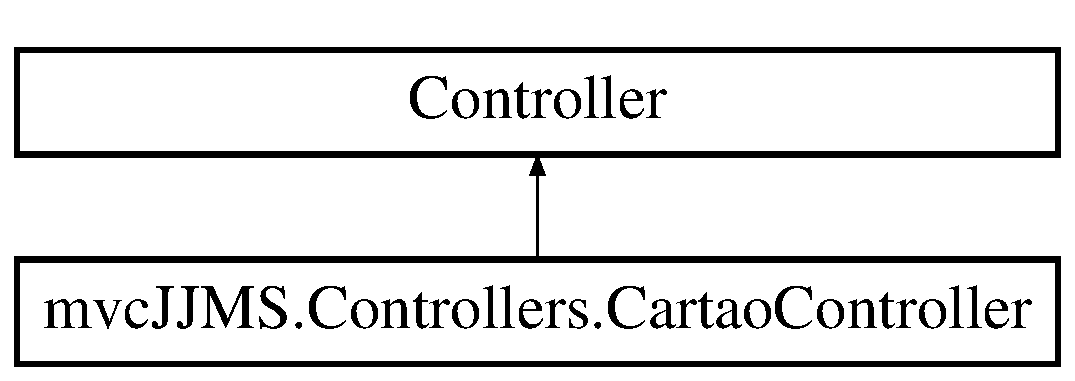
\includegraphics[height=2.000000cm]{classmvc_j_j_m_s_1_1_controllers_1_1_cartao_controller}
\end{center}
\end{figure}
\subsection*{Public Member Functions}
\begin{DoxyCompactItemize}
\item 
\mbox{\Hypertarget{classmvc_j_j_m_s_1_1_controllers_1_1_cartao_controller_acd5089f69da95c88587b994307362ade}\label{classmvc_j_j_m_s_1_1_controllers_1_1_cartao_controller_acd5089f69da95c88587b994307362ade}} 
{\bfseries Cartao\+Controller} (\mbox{\hyperlink{classmvc_j_j_m_s_1_1_data_1_1_j_j_m_s_context}{J\+J\+M\+S\+Context}} context)
\item 
bool \mbox{\hyperlink{classmvc_j_j_m_s_1_1_controllers_1_1_cartao_controller_a1e60f8ebecc93f7210c7e8a143c2e965}{Luhn\+\_\+check}} (long num\+Cart\+Credito)
\begin{DoxyCompactList}\small\item\em checks if a number of credit card respects the luhn algoritm \end{DoxyCompactList}\item 
bool \mbox{\hyperlink{classmvc_j_j_m_s_1_1_controllers_1_1_cartao_controller_a1e57d6690edbfa272d61c72e3e2f945b}{Cartao\+Valido}} (long num\+Cart\+Credito, int mes, int ano, int cvv, string pais)
\begin{DoxyCompactList}\small\item\em Verify is Cartao\+Credito is valid, aplies luhn algoritm, checks validate and if cvv have 3 or 4 of length \end{DoxyCompactList}\end{DoxyCompactItemize}


\subsection{Member Function Documentation}
\mbox{\Hypertarget{classmvc_j_j_m_s_1_1_controllers_1_1_cartao_controller_a1e57d6690edbfa272d61c72e3e2f945b}\label{classmvc_j_j_m_s_1_1_controllers_1_1_cartao_controller_a1e57d6690edbfa272d61c72e3e2f945b}} 
\index{mvc\+J\+J\+M\+S\+::\+Controllers\+::\+Cartao\+Controller@{mvc\+J\+J\+M\+S\+::\+Controllers\+::\+Cartao\+Controller}!Cartao\+Valido@{Cartao\+Valido}}
\index{Cartao\+Valido@{Cartao\+Valido}!mvc\+J\+J\+M\+S\+::\+Controllers\+::\+Cartao\+Controller@{mvc\+J\+J\+M\+S\+::\+Controllers\+::\+Cartao\+Controller}}
\subsubsection{\texorpdfstring{Cartao\+Valido()}{CartaoValido()}}
{\footnotesize\ttfamily bool mvc\+J\+J\+M\+S.\+Controllers.\+Cartao\+Controller.\+Cartao\+Valido (\begin{DoxyParamCaption}\item[{long}]{num\+Cart\+Credito,  }\item[{int}]{mes,  }\item[{int}]{ano,  }\item[{int}]{cvv,  }\item[{string}]{pais }\end{DoxyParamCaption})\hspace{0.3cm}{\ttfamily [inline]}}



Verify is Cartao\+Credito is valid, aplies luhn algoritm, checks validate and if cvv have 3 or 4 of length 


\begin{DoxyParams}{Parameters}
{\em num\+Cart\+Credito} & \\
\hline
{\em mes} & \\
\hline
{\em ano} & \\
\hline
{\em cvv} & \\
\hline
{\em pais} & \\
\hline
\end{DoxyParams}
\begin{DoxyReturn}{Returns}
true if Cartao\+Credito is valid, false if not
\end{DoxyReturn}
\mbox{\Hypertarget{classmvc_j_j_m_s_1_1_controllers_1_1_cartao_controller_a1e60f8ebecc93f7210c7e8a143c2e965}\label{classmvc_j_j_m_s_1_1_controllers_1_1_cartao_controller_a1e60f8ebecc93f7210c7e8a143c2e965}} 
\index{mvc\+J\+J\+M\+S\+::\+Controllers\+::\+Cartao\+Controller@{mvc\+J\+J\+M\+S\+::\+Controllers\+::\+Cartao\+Controller}!Luhn\+\_\+check@{Luhn\+\_\+check}}
\index{Luhn\+\_\+check@{Luhn\+\_\+check}!mvc\+J\+J\+M\+S\+::\+Controllers\+::\+Cartao\+Controller@{mvc\+J\+J\+M\+S\+::\+Controllers\+::\+Cartao\+Controller}}
\subsubsection{\texorpdfstring{Luhn\+\_\+check()}{Luhn\_check()}}
{\footnotesize\ttfamily bool mvc\+J\+J\+M\+S.\+Controllers.\+Cartao\+Controller.\+Luhn\+\_\+check (\begin{DoxyParamCaption}\item[{long}]{num\+Cart\+Credito }\end{DoxyParamCaption})\hspace{0.3cm}{\ttfamily [inline]}}



checks if a number of credit card respects the luhn algoritm 


\begin{DoxyParams}{Parameters}
{\em num\+Cart\+Credito} & \\
\hline
\end{DoxyParams}
\begin{DoxyReturn}{Returns}
true if is valid, false if not
\end{DoxyReturn}


The documentation for this class was generated from the following file\+:\begin{DoxyCompactItemize}
\item 
Controllers/Cartao\+Controller.\+cs\end{DoxyCompactItemize}

\hypertarget{classmvc_j_j_m_s_1_1_models_1_1_cartao_credito}{}\section{mvc\+J\+J\+M\+S.\+Models.\+Cartao\+Credito Class Reference}
\label{classmvc_j_j_m_s_1_1_models_1_1_cartao_credito}\index{mvc\+J\+J\+M\+S.\+Models.\+Cartao\+Credito@{mvc\+J\+J\+M\+S.\+Models.\+Cartao\+Credito}}


Represents a Credit Card used to pay for the costs associated with an order  


\subsection*{Public Member Functions}
\begin{DoxyCompactItemize}
\item 
bool \mbox{\hyperlink{classmvc_j_j_m_s_1_1_models_1_1_cartao_credito_ab5535ad2253ef9ed12be8109615de9af}{Pagamento}} ()
\begin{DoxyCompactList}\small\item\em Payment realization with credit card \end{DoxyCompactList}\end{DoxyCompactItemize}
\subsection*{Properties}
\begin{DoxyCompactItemize}
\item 
\mbox{\Hypertarget{classmvc_j_j_m_s_1_1_models_1_1_cartao_credito_a304fc1eca4898a98c28975430cff7e20}\label{classmvc_j_j_m_s_1_1_models_1_1_cartao_credito_a304fc1eca4898a98c28975430cff7e20}} 
long {\bfseries Cartao\+Credito\+ID}\hspace{0.3cm}{\ttfamily  \mbox{[}get, set\mbox{]}}
\item 
\mbox{\Hypertarget{classmvc_j_j_m_s_1_1_models_1_1_cartao_credito_a2e757f644e2762e54d20c57aa5f48a04}\label{classmvc_j_j_m_s_1_1_models_1_1_cartao_credito_a2e757f644e2762e54d20c57aa5f48a04}} 
int {\bfseries mes}\hspace{0.3cm}{\ttfamily  \mbox{[}get, set\mbox{]}}
\item 
\mbox{\Hypertarget{classmvc_j_j_m_s_1_1_models_1_1_cartao_credito_ad1773cf8f0bf7c9d564f2bf74d53c228}\label{classmvc_j_j_m_s_1_1_models_1_1_cartao_credito_ad1773cf8f0bf7c9d564f2bf74d53c228}} 
int {\bfseries ano}\hspace{0.3cm}{\ttfamily  \mbox{[}get, set\mbox{]}}
\item 
\mbox{\Hypertarget{classmvc_j_j_m_s_1_1_models_1_1_cartao_credito_ad30f2e84be8bd2933bb8a5181c0082f8}\label{classmvc_j_j_m_s_1_1_models_1_1_cartao_credito_ad30f2e84be8bd2933bb8a5181c0082f8}} 
int {\bfseries cvv}\hspace{0.3cm}{\ttfamily  \mbox{[}get, set\mbox{]}}
\item 
\mbox{\Hypertarget{classmvc_j_j_m_s_1_1_models_1_1_cartao_credito_ab9e08c39bd28c27e338ee6c3aa4a53f4}\label{classmvc_j_j_m_s_1_1_models_1_1_cartao_credito_ab9e08c39bd28c27e338ee6c3aa4a53f4}} 
string {\bfseries pais}\hspace{0.3cm}{\ttfamily  \mbox{[}get, set\mbox{]}}
\item 
\mbox{\Hypertarget{classmvc_j_j_m_s_1_1_models_1_1_cartao_credito_a9c1a277598a6e137fcb228e4803cec2e}\label{classmvc_j_j_m_s_1_1_models_1_1_cartao_credito_a9c1a277598a6e137fcb228e4803cec2e}} 
I\+Collection$<$ \mbox{\hyperlink{classmvc_j_j_m_s_1_1_models_1_1_encomenda}{Encomenda}} $>$ {\bfseries Encomendas}\hspace{0.3cm}{\ttfamily  \mbox{[}get, set\mbox{]}}
\end{DoxyCompactItemize}


\subsection{Detailed Description}
Represents a Credit Card used to pay for the costs associated with an order 



\subsection{Member Function Documentation}
\mbox{\Hypertarget{classmvc_j_j_m_s_1_1_models_1_1_cartao_credito_ab5535ad2253ef9ed12be8109615de9af}\label{classmvc_j_j_m_s_1_1_models_1_1_cartao_credito_ab5535ad2253ef9ed12be8109615de9af}} 
\index{mvc\+J\+J\+M\+S\+::\+Models\+::\+Cartao\+Credito@{mvc\+J\+J\+M\+S\+::\+Models\+::\+Cartao\+Credito}!Pagamento@{Pagamento}}
\index{Pagamento@{Pagamento}!mvc\+J\+J\+M\+S\+::\+Models\+::\+Cartao\+Credito@{mvc\+J\+J\+M\+S\+::\+Models\+::\+Cartao\+Credito}}
\subsubsection{\texorpdfstring{Pagamento()}{Pagamento()}}
{\footnotesize\ttfamily bool mvc\+J\+J\+M\+S.\+Models.\+Cartao\+Credito.\+Pagamento (\begin{DoxyParamCaption}{ }\end{DoxyParamCaption})\hspace{0.3cm}{\ttfamily [inline]}}



Payment realization with credit card 

\begin{DoxyReturn}{Returns}
T\+R\+UE if payment is correctly done, else F\+A\+L\+SE
\end{DoxyReturn}


The documentation for this class was generated from the following file\+:\begin{DoxyCompactItemize}
\item 
Models/Cartao\+Credito.\+cs\end{DoxyCompactItemize}

\hypertarget{classmvc_j_j_m_s_1_1_models_1_1_cliente}{}\section{mvc\+J\+J\+M\+S.\+Models.\+Cliente Class Reference}
\label{classmvc_j_j_m_s_1_1_models_1_1_cliente}\index{mvc\+J\+J\+M\+S.\+Models.\+Cliente@{mvc\+J\+J\+M\+S.\+Models.\+Cliente}}


Represents a user of type Client  


Inheritance diagram for mvc\+J\+J\+M\+S.\+Models.\+Cliente\+:\begin{figure}[H]
\begin{center}
\leavevmode
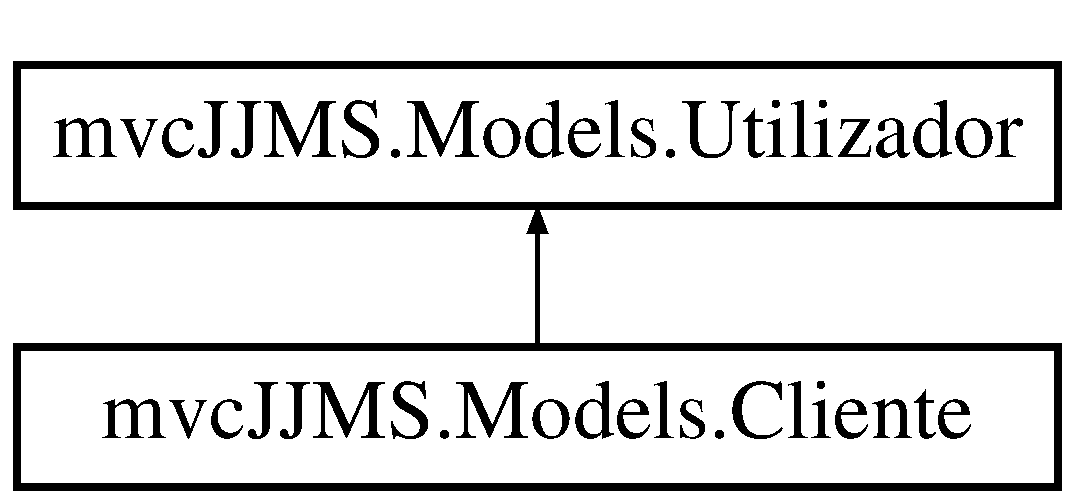
\includegraphics[height=2.000000cm]{classmvc_j_j_m_s_1_1_models_1_1_cliente}
\end{center}
\end{figure}
\subsection*{Public Member Functions}
\begin{DoxyCompactItemize}
\item 
bool \mbox{\hyperlink{classmvc_j_j_m_s_1_1_models_1_1_cliente_a1071410f6080091b9996277cba83f0b4}{Tem\+Encomenda}} (int id\+Encomenda)
\begin{DoxyCompactList}\small\item\em Checks if client is associated with a given order \end{DoxyCompactList}\item 
void \mbox{\hyperlink{classmvc_j_j_m_s_1_1_models_1_1_cliente_ae2c56c8d9c14db342234852e07873147}{Bloqueia}} ()
\begin{DoxyCompactList}\small\item\em Method used to block client \end{DoxyCompactList}\item 
int \mbox{\hyperlink{classmvc_j_j_m_s_1_1_models_1_1_cliente_af711f052377f6684bc93ac4886d20a78}{get\+Utilizador\+ID}} ()
\begin{DoxyCompactList}\small\item\em Retrieves unique identifier of client \end{DoxyCompactList}\end{DoxyCompactItemize}
\subsection*{Properties}
\begin{DoxyCompactItemize}
\item 
\mbox{\Hypertarget{classmvc_j_j_m_s_1_1_models_1_1_cliente_a6bf7993bd0beaa8c680b83f8e725f903}\label{classmvc_j_j_m_s_1_1_models_1_1_cliente_a6bf7993bd0beaa8c680b83f8e725f903}} 
string {\bfseries Morada}\hspace{0.3cm}{\ttfamily  \mbox{[}get, set\mbox{]}}
\item 
\mbox{\Hypertarget{classmvc_j_j_m_s_1_1_models_1_1_cliente_a0b2c56229883d355575e444426ac3fbc}\label{classmvc_j_j_m_s_1_1_models_1_1_cliente_a0b2c56229883d355575e444426ac3fbc}} 
string {\bfseries Telefone}\hspace{0.3cm}{\ttfamily  \mbox{[}get, set\mbox{]}}
\item 
\mbox{\Hypertarget{classmvc_j_j_m_s_1_1_models_1_1_cliente_a2017f6f64f03dd51c61bfcc7c40a7eb8}\label{classmvc_j_j_m_s_1_1_models_1_1_cliente_a2017f6f64f03dd51c61bfcc7c40a7eb8}} 
bool {\bfseries Bloqueado}\hspace{0.3cm}{\ttfamily  \mbox{[}get, set\mbox{]}}
\item 
\mbox{\Hypertarget{classmvc_j_j_m_s_1_1_models_1_1_cliente_a1424f8c7942aee89e4b1b91919c6affc}\label{classmvc_j_j_m_s_1_1_models_1_1_cliente_a1424f8c7942aee89e4b1b91919c6affc}} 
I\+Collection$<$ \mbox{\hyperlink{classmvc_j_j_m_s_1_1_models_1_1_encomenda}{Encomenda}} $>$ {\bfseries Encomendas}\hspace{0.3cm}{\ttfamily  \mbox{[}get, set\mbox{]}}
\end{DoxyCompactItemize}


\subsection{Detailed Description}
Represents a user of type Client 



\subsection{Member Function Documentation}
\mbox{\Hypertarget{classmvc_j_j_m_s_1_1_models_1_1_cliente_ae2c56c8d9c14db342234852e07873147}\label{classmvc_j_j_m_s_1_1_models_1_1_cliente_ae2c56c8d9c14db342234852e07873147}} 
\index{mvc\+J\+J\+M\+S\+::\+Models\+::\+Cliente@{mvc\+J\+J\+M\+S\+::\+Models\+::\+Cliente}!Bloqueia@{Bloqueia}}
\index{Bloqueia@{Bloqueia}!mvc\+J\+J\+M\+S\+::\+Models\+::\+Cliente@{mvc\+J\+J\+M\+S\+::\+Models\+::\+Cliente}}
\subsubsection{\texorpdfstring{Bloqueia()}{Bloqueia()}}
{\footnotesize\ttfamily void mvc\+J\+J\+M\+S.\+Models.\+Cliente.\+Bloqueia (\begin{DoxyParamCaption}{ }\end{DoxyParamCaption})\hspace{0.3cm}{\ttfamily [inline]}}



Method used to block client 

\mbox{\Hypertarget{classmvc_j_j_m_s_1_1_models_1_1_cliente_af711f052377f6684bc93ac4886d20a78}\label{classmvc_j_j_m_s_1_1_models_1_1_cliente_af711f052377f6684bc93ac4886d20a78}} 
\index{mvc\+J\+J\+M\+S\+::\+Models\+::\+Cliente@{mvc\+J\+J\+M\+S\+::\+Models\+::\+Cliente}!get\+Utilizador\+ID@{get\+Utilizador\+ID}}
\index{get\+Utilizador\+ID@{get\+Utilizador\+ID}!mvc\+J\+J\+M\+S\+::\+Models\+::\+Cliente@{mvc\+J\+J\+M\+S\+::\+Models\+::\+Cliente}}
\subsubsection{\texorpdfstring{get\+Utilizador\+I\+D()}{getUtilizadorID()}}
{\footnotesize\ttfamily int mvc\+J\+J\+M\+S.\+Models.\+Cliente.\+get\+Utilizador\+ID (\begin{DoxyParamCaption}{ }\end{DoxyParamCaption})\hspace{0.3cm}{\ttfamily [inline]}}



Retrieves unique identifier of client 

\begin{DoxyReturn}{Returns}
Client unique identifier
\end{DoxyReturn}
\mbox{\Hypertarget{classmvc_j_j_m_s_1_1_models_1_1_cliente_a1071410f6080091b9996277cba83f0b4}\label{classmvc_j_j_m_s_1_1_models_1_1_cliente_a1071410f6080091b9996277cba83f0b4}} 
\index{mvc\+J\+J\+M\+S\+::\+Models\+::\+Cliente@{mvc\+J\+J\+M\+S\+::\+Models\+::\+Cliente}!Tem\+Encomenda@{Tem\+Encomenda}}
\index{Tem\+Encomenda@{Tem\+Encomenda}!mvc\+J\+J\+M\+S\+::\+Models\+::\+Cliente@{mvc\+J\+J\+M\+S\+::\+Models\+::\+Cliente}}
\subsubsection{\texorpdfstring{Tem\+Encomenda()}{TemEncomenda()}}
{\footnotesize\ttfamily bool mvc\+J\+J\+M\+S.\+Models.\+Cliente.\+Tem\+Encomenda (\begin{DoxyParamCaption}\item[{int}]{id\+Encomenda }\end{DoxyParamCaption})\hspace{0.3cm}{\ttfamily [inline]}}



Checks if client is associated with a given order 


\begin{DoxyParams}{Parameters}
{\em id\+Encomenda} & Unique identifier for a single order\\
\hline
\end{DoxyParams}
\begin{DoxyReturn}{Returns}
T\+R\+UE if client is associated with order, else F\+A\+L\+SE
\end{DoxyReturn}


The documentation for this class was generated from the following file\+:\begin{DoxyCompactItemize}
\item 
Models/Cliente.\+cs\end{DoxyCompactItemize}

\hypertarget{classmvc_j_j_m_s_1_1_controllers_1_1_cliente_controller}{}\section{mvc\+J\+J\+M\+S.\+Controllers.\+Cliente\+Controller Class Reference}
\label{classmvc_j_j_m_s_1_1_controllers_1_1_cliente_controller}\index{mvc\+J\+J\+M\+S.\+Controllers.\+Cliente\+Controller@{mvc\+J\+J\+M\+S.\+Controllers.\+Cliente\+Controller}}
Inheritance diagram for mvc\+J\+J\+M\+S.\+Controllers.\+Cliente\+Controller\+:\begin{figure}[H]
\begin{center}
\leavevmode
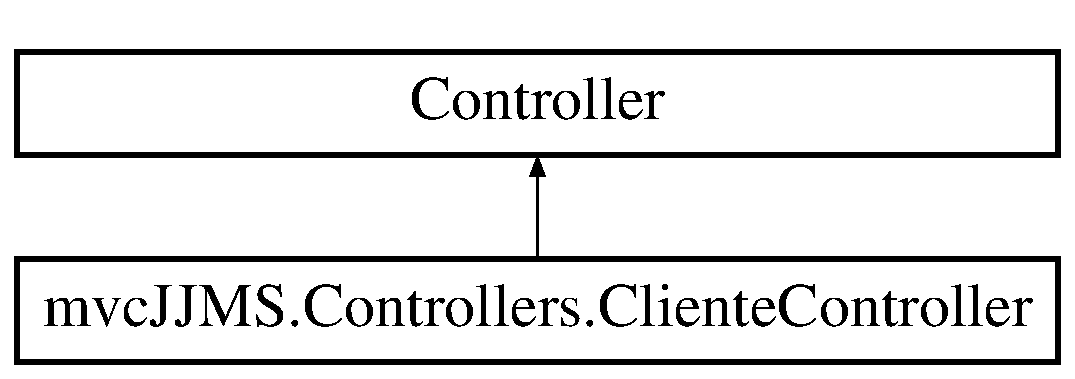
\includegraphics[height=2.000000cm]{classmvc_j_j_m_s_1_1_controllers_1_1_cliente_controller}
\end{center}
\end{figure}
\subsection*{Public Member Functions}
\begin{DoxyCompactItemize}
\item 
\mbox{\Hypertarget{classmvc_j_j_m_s_1_1_controllers_1_1_cliente_controller_a55a36c3b859c2bbabf552b1526c18cef}\label{classmvc_j_j_m_s_1_1_controllers_1_1_cliente_controller_a55a36c3b859c2bbabf552b1526c18cef}} 
{\bfseries Cliente\+Controller} (\mbox{\hyperlink{classmvc_j_j_m_s_1_1_data_1_1_j_j_m_s_context}{J\+J\+M\+S\+Context}} context, \mbox{\hyperlink{classmvc_j_j_m_s_1_1_controllers_1_1_utilizador_controller}{Utilizador\+Controller}} u\+Controller)
\item 
Action\+Result \mbox{\hyperlink{classmvc_j_j_m_s_1_1_controllers_1_1_cliente_controller_a31325ea0231ffa6f09996a9f61f1731b}{Registar}} (string user, string password, string email, string morada, string telefone)
\begin{DoxyCompactList}\small\item\em Checks input and if all is right, save the Cliente to the Data\+Base \end{DoxyCompactList}\item 
bool \mbox{\hyperlink{classmvc_j_j_m_s_1_1_controllers_1_1_cliente_controller_a55f13fda1a4342595d427b8bfc9a2978}{telefone\+Valido}} (string telefone)
\begin{DoxyCompactList}\small\item\em Checks if a string is a valid phone number \end{DoxyCompactList}\item 
bool \mbox{\hyperlink{classmvc_j_j_m_s_1_1_controllers_1_1_cliente_controller_a0027e8277cd9552a1122e12547ec10c6}{password\+Segura}} (string password)
\begin{DoxyCompactList}\small\item\em Checks if a password is safe enough for the company \end{DoxyCompactList}\item 
bool \mbox{\hyperlink{classmvc_j_j_m_s_1_1_controllers_1_1_cliente_controller_a0f8b63358a35d40ad0bdda9442d9a677}{email\+Valido}} (string email)
\begin{DoxyCompactList}\small\item\em Checks if a string is a valid email \end{DoxyCompactList}\item 
string \mbox{\hyperlink{classmvc_j_j_m_s_1_1_controllers_1_1_cliente_controller_a6925f8c7f2234512eceb9e027c987ca9}{Get\+Cliente\+Morada}} (int id\+Cliente)
\begin{DoxyCompactList}\small\item\em Retrieves the address associated with a client \end{DoxyCompactList}\item 
string \mbox{\hyperlink{classmvc_j_j_m_s_1_1_controllers_1_1_cliente_controller_ac50b76017495e8df860bffad1e7ea29f}{Get\+Cliente\+Telefone}} (int id\+Cliente)
\begin{DoxyCompactList}\small\item\em Retrieves the phone number associated with a client \end{DoxyCompactList}\item 
void \mbox{\hyperlink{classmvc_j_j_m_s_1_1_controllers_1_1_cliente_controller_a27719253428ef9593690de0afdba5596}{Update\+Morada}} (int id\+Cliente, string morada\+Input)
\begin{DoxyCompactList}\small\item\em Updates the address of a client \end{DoxyCompactList}\item 
void \mbox{\hyperlink{classmvc_j_j_m_s_1_1_controllers_1_1_cliente_controller_aefbf9f1512ccb78afa9acaef47b95b98}{Update\+Telefone}} (int id\+Cliente, string telefone\+Input)
\begin{DoxyCompactList}\small\item\em Updates the phone number of a client \end{DoxyCompactList}\item 
void \mbox{\hyperlink{classmvc_j_j_m_s_1_1_controllers_1_1_cliente_controller_a75678bb2dcb7f48853343d9bf898d64a}{Bloquear}} (int id\+Cliente)
\begin{DoxyCompactList}\small\item\em Blocks a particular client \end{DoxyCompactList}\item 
bool \mbox{\hyperlink{classmvc_j_j_m_s_1_1_controllers_1_1_cliente_controller_a71e4b089bf6844fd8440ae4571bb6ae0}{Transfere\+Montante}} (int id\+Cliente, int id\+Encomenda)
\begin{DoxyCompactList}\small\item\em Performs payment for a given order \end{DoxyCompactList}\item 
void \mbox{\hyperlink{classmvc_j_j_m_s_1_1_controllers_1_1_cliente_controller_a626d408a5094fabc40454be45b143ab2}{Gerar\+Fatura}} (int id\+Cliente, int id\+Encomenda)
\begin{DoxyCompactList}\small\item\em Generates order details for a given order \end{DoxyCompactList}\item 
F\+I\+LE \mbox{\hyperlink{classmvc_j_j_m_s_1_1_controllers_1_1_cliente_controller_afa8996759fcf65477a9aac44cd0c9810}{Get\+Fatura}} (int id\+Cliente, int id\+Encomenda)
\begin{DoxyCompactList}\small\item\em Retrieves order details associated with a given order \end{DoxyCompactList}\item 
async Task$<$ List$<$ \mbox{\hyperlink{classmvc_j_j_m_s_1_1_models_1_1_encomenda}{Encomenda}} $>$ $>$ \mbox{\hyperlink{classmvc_j_j_m_s_1_1_controllers_1_1_cliente_controller_a2023d96fe1797ec7673210da1233dfe2}{Get\+Historico\+Enc}} (int id\+Cliente)
\begin{DoxyCompactList}\small\item\em Retrieves a client\textquotesingle{}s order history \end{DoxyCompactList}\item 
bool \mbox{\hyperlink{classmvc_j_j_m_s_1_1_controllers_1_1_cliente_controller_a5ab387b5c0be1e73a0ec1c468cc3ac5e}{Existe\+Encomenda\+Cliente}} (int id\+Cliente, int id\+Encomenda)
\begin{DoxyCompactList}\small\item\em Checks if a given order is associated with a certain client \end{DoxyCompactList}\item 
bool \mbox{\hyperlink{classmvc_j_j_m_s_1_1_controllers_1_1_cliente_controller_ab916e41bf8757268e95796c1cf86d3df}{Esta\+Bloqueado}} (int id\+Cliente)
\begin{DoxyCompactList}\small\item\em Checks if a given client is blocked \end{DoxyCompactList}\item 
\mbox{\Hypertarget{classmvc_j_j_m_s_1_1_controllers_1_1_cliente_controller_abe5a6649f29f0a35046839bad04523ef}\label{classmvc_j_j_m_s_1_1_controllers_1_1_cliente_controller_abe5a6649f29f0a35046839bad04523ef}} 
View\+Result {\bfseries Email\+Em\+Uso} ()
\item 
\mbox{\Hypertarget{classmvc_j_j_m_s_1_1_controllers_1_1_cliente_controller_a5fcddb32b175cb22a90b8dbaca7a45bb}\label{classmvc_j_j_m_s_1_1_controllers_1_1_cliente_controller_a5fcddb32b175cb22a90b8dbaca7a45bb}} 
View\+Result {\bfseries Password\+Insegura} ()
\item 
\mbox{\Hypertarget{classmvc_j_j_m_s_1_1_controllers_1_1_cliente_controller_aa66f3fb47fd4c21a67514ef6a38a8390}\label{classmvc_j_j_m_s_1_1_controllers_1_1_cliente_controller_aa66f3fb47fd4c21a67514ef6a38a8390}} 
View\+Result {\bfseries Email\+Invalido} ()
\item 
\mbox{\Hypertarget{classmvc_j_j_m_s_1_1_controllers_1_1_cliente_controller_ab65d2ba3cdb037df769d23b70216749d}\label{classmvc_j_j_m_s_1_1_controllers_1_1_cliente_controller_ab65d2ba3cdb037df769d23b70216749d}} 
View\+Result {\bfseries Sucesso} ()
\item 
\mbox{\Hypertarget{classmvc_j_j_m_s_1_1_controllers_1_1_cliente_controller_a8d1e06b92f61ed481fa342837fcd2e7f}\label{classmvc_j_j_m_s_1_1_controllers_1_1_cliente_controller_a8d1e06b92f61ed481fa342837fcd2e7f}} 
View\+Result {\bfseries Telefone\+Invalido} ()
\item 
\mbox{\Hypertarget{classmvc_j_j_m_s_1_1_controllers_1_1_cliente_controller_a0043cef3a9faa31c164bfba141b5d22b}\label{classmvc_j_j_m_s_1_1_controllers_1_1_cliente_controller_a0043cef3a9faa31c164bfba141b5d22b}} 
View\+Result {\bfseries Cancelar} ()
\item 
void \mbox{\hyperlink{classmvc_j_j_m_s_1_1_controllers_1_1_cliente_controller_ac3bcc6f76f48dfc5553f1686e2f44dd5}{Pagar\+Serviço}} (int id\+Cliente, int id\+Encomenda)
\begin{DoxyCompactList}\small\item\em Performs payment for a given order and client, if the payment isn\textquotesingle{}t successfully it blocks the client \end{DoxyCompactList}\end{DoxyCompactItemize}


\subsection{Member Function Documentation}
\mbox{\Hypertarget{classmvc_j_j_m_s_1_1_controllers_1_1_cliente_controller_a75678bb2dcb7f48853343d9bf898d64a}\label{classmvc_j_j_m_s_1_1_controllers_1_1_cliente_controller_a75678bb2dcb7f48853343d9bf898d64a}} 
\index{mvc\+J\+J\+M\+S\+::\+Controllers\+::\+Cliente\+Controller@{mvc\+J\+J\+M\+S\+::\+Controllers\+::\+Cliente\+Controller}!Bloquear@{Bloquear}}
\index{Bloquear@{Bloquear}!mvc\+J\+J\+M\+S\+::\+Controllers\+::\+Cliente\+Controller@{mvc\+J\+J\+M\+S\+::\+Controllers\+::\+Cliente\+Controller}}
\subsubsection{\texorpdfstring{Bloquear()}{Bloquear()}}
{\footnotesize\ttfamily void mvc\+J\+J\+M\+S.\+Controllers.\+Cliente\+Controller.\+Bloquear (\begin{DoxyParamCaption}\item[{int}]{id\+Cliente }\end{DoxyParamCaption})\hspace{0.3cm}{\ttfamily [inline]}}



Blocks a particular client 


\begin{DoxyParams}{Parameters}
{\em id\+Cliente} & Unique identifier for a client to block\\
\hline
\end{DoxyParams}
\mbox{\Hypertarget{classmvc_j_j_m_s_1_1_controllers_1_1_cliente_controller_a0f8b63358a35d40ad0bdda9442d9a677}\label{classmvc_j_j_m_s_1_1_controllers_1_1_cliente_controller_a0f8b63358a35d40ad0bdda9442d9a677}} 
\index{mvc\+J\+J\+M\+S\+::\+Controllers\+::\+Cliente\+Controller@{mvc\+J\+J\+M\+S\+::\+Controllers\+::\+Cliente\+Controller}!email\+Valido@{email\+Valido}}
\index{email\+Valido@{email\+Valido}!mvc\+J\+J\+M\+S\+::\+Controllers\+::\+Cliente\+Controller@{mvc\+J\+J\+M\+S\+::\+Controllers\+::\+Cliente\+Controller}}
\subsubsection{\texorpdfstring{email\+Valido()}{emailValido()}}
{\footnotesize\ttfamily bool mvc\+J\+J\+M\+S.\+Controllers.\+Cliente\+Controller.\+email\+Valido (\begin{DoxyParamCaption}\item[{string}]{email }\end{DoxyParamCaption})\hspace{0.3cm}{\ttfamily [inline]}}



Checks if a string is a valid email 


\begin{DoxyParams}{Parameters}
{\em email} & string email to analyze\\
\hline
\end{DoxyParams}
\begin{DoxyReturn}{Returns}
T\+R\+UE if the string is a email, else F\+A\+L\+SE
\end{DoxyReturn}
\mbox{\Hypertarget{classmvc_j_j_m_s_1_1_controllers_1_1_cliente_controller_ab916e41bf8757268e95796c1cf86d3df}\label{classmvc_j_j_m_s_1_1_controllers_1_1_cliente_controller_ab916e41bf8757268e95796c1cf86d3df}} 
\index{mvc\+J\+J\+M\+S\+::\+Controllers\+::\+Cliente\+Controller@{mvc\+J\+J\+M\+S\+::\+Controllers\+::\+Cliente\+Controller}!Esta\+Bloqueado@{Esta\+Bloqueado}}
\index{Esta\+Bloqueado@{Esta\+Bloqueado}!mvc\+J\+J\+M\+S\+::\+Controllers\+::\+Cliente\+Controller@{mvc\+J\+J\+M\+S\+::\+Controllers\+::\+Cliente\+Controller}}
\subsubsection{\texorpdfstring{Esta\+Bloqueado()}{EstaBloqueado()}}
{\footnotesize\ttfamily bool mvc\+J\+J\+M\+S.\+Controllers.\+Cliente\+Controller.\+Esta\+Bloqueado (\begin{DoxyParamCaption}\item[{int}]{id\+Cliente }\end{DoxyParamCaption})\hspace{0.3cm}{\ttfamily [inline]}}



Checks if a given client is blocked 


\begin{DoxyParams}{Parameters}
{\em id\+Cliente} & Unique identifier for a client\\
\hline
\end{DoxyParams}
\begin{DoxyReturn}{Returns}
T\+R\+UE if the client is blocked, else F\+A\+L\+SE
\end{DoxyReturn}
\mbox{\Hypertarget{classmvc_j_j_m_s_1_1_controllers_1_1_cliente_controller_a5ab387b5c0be1e73a0ec1c468cc3ac5e}\label{classmvc_j_j_m_s_1_1_controllers_1_1_cliente_controller_a5ab387b5c0be1e73a0ec1c468cc3ac5e}} 
\index{mvc\+J\+J\+M\+S\+::\+Controllers\+::\+Cliente\+Controller@{mvc\+J\+J\+M\+S\+::\+Controllers\+::\+Cliente\+Controller}!Existe\+Encomenda\+Cliente@{Existe\+Encomenda\+Cliente}}
\index{Existe\+Encomenda\+Cliente@{Existe\+Encomenda\+Cliente}!mvc\+J\+J\+M\+S\+::\+Controllers\+::\+Cliente\+Controller@{mvc\+J\+J\+M\+S\+::\+Controllers\+::\+Cliente\+Controller}}
\subsubsection{\texorpdfstring{Existe\+Encomenda\+Cliente()}{ExisteEncomendaCliente()}}
{\footnotesize\ttfamily bool mvc\+J\+J\+M\+S.\+Controllers.\+Cliente\+Controller.\+Existe\+Encomenda\+Cliente (\begin{DoxyParamCaption}\item[{int}]{id\+Cliente,  }\item[{int}]{id\+Encomenda }\end{DoxyParamCaption})\hspace{0.3cm}{\ttfamily [inline]}}



Checks if a given order is associated with a certain client 


\begin{DoxyParams}{Parameters}
{\em id\+Cliente} & Unique identifier for a client\\
\hline
{\em id\+Encomenda} & Unique identifier for a single order\\
\hline
\end{DoxyParams}
\begin{DoxyReturn}{Returns}
T\+R\+UE if the order is associated, else F\+A\+L\+SE
\end{DoxyReturn}
\mbox{\Hypertarget{classmvc_j_j_m_s_1_1_controllers_1_1_cliente_controller_a626d408a5094fabc40454be45b143ab2}\label{classmvc_j_j_m_s_1_1_controllers_1_1_cliente_controller_a626d408a5094fabc40454be45b143ab2}} 
\index{mvc\+J\+J\+M\+S\+::\+Controllers\+::\+Cliente\+Controller@{mvc\+J\+J\+M\+S\+::\+Controllers\+::\+Cliente\+Controller}!Gerar\+Fatura@{Gerar\+Fatura}}
\index{Gerar\+Fatura@{Gerar\+Fatura}!mvc\+J\+J\+M\+S\+::\+Controllers\+::\+Cliente\+Controller@{mvc\+J\+J\+M\+S\+::\+Controllers\+::\+Cliente\+Controller}}
\subsubsection{\texorpdfstring{Gerar\+Fatura()}{GerarFatura()}}
{\footnotesize\ttfamily void mvc\+J\+J\+M\+S.\+Controllers.\+Cliente\+Controller.\+Gerar\+Fatura (\begin{DoxyParamCaption}\item[{int}]{id\+Cliente,  }\item[{int}]{id\+Encomenda }\end{DoxyParamCaption})\hspace{0.3cm}{\ttfamily [inline]}}



Generates order details for a given order 


\begin{DoxyParams}{Parameters}
{\em id\+Cliente} & Unique identifier for a client\\
\hline
{\em id\+Encomenda} & Unique identifier for a single order\\
\hline
\end{DoxyParams}
\mbox{\Hypertarget{classmvc_j_j_m_s_1_1_controllers_1_1_cliente_controller_a6925f8c7f2234512eceb9e027c987ca9}\label{classmvc_j_j_m_s_1_1_controllers_1_1_cliente_controller_a6925f8c7f2234512eceb9e027c987ca9}} 
\index{mvc\+J\+J\+M\+S\+::\+Controllers\+::\+Cliente\+Controller@{mvc\+J\+J\+M\+S\+::\+Controllers\+::\+Cliente\+Controller}!Get\+Cliente\+Morada@{Get\+Cliente\+Morada}}
\index{Get\+Cliente\+Morada@{Get\+Cliente\+Morada}!mvc\+J\+J\+M\+S\+::\+Controllers\+::\+Cliente\+Controller@{mvc\+J\+J\+M\+S\+::\+Controllers\+::\+Cliente\+Controller}}
\subsubsection{\texorpdfstring{Get\+Cliente\+Morada()}{GetClienteMorada()}}
{\footnotesize\ttfamily string mvc\+J\+J\+M\+S.\+Controllers.\+Cliente\+Controller.\+Get\+Cliente\+Morada (\begin{DoxyParamCaption}\item[{int}]{id\+Cliente }\end{DoxyParamCaption})\hspace{0.3cm}{\ttfamily [inline]}}



Retrieves the address associated with a client 


\begin{DoxyParams}{Parameters}
{\em id\+Cliente} & Unique identifier for a client\\
\hline
\end{DoxyParams}
\begin{DoxyReturn}{Returns}
Client address
\end{DoxyReturn}
\mbox{\Hypertarget{classmvc_j_j_m_s_1_1_controllers_1_1_cliente_controller_ac50b76017495e8df860bffad1e7ea29f}\label{classmvc_j_j_m_s_1_1_controllers_1_1_cliente_controller_ac50b76017495e8df860bffad1e7ea29f}} 
\index{mvc\+J\+J\+M\+S\+::\+Controllers\+::\+Cliente\+Controller@{mvc\+J\+J\+M\+S\+::\+Controllers\+::\+Cliente\+Controller}!Get\+Cliente\+Telefone@{Get\+Cliente\+Telefone}}
\index{Get\+Cliente\+Telefone@{Get\+Cliente\+Telefone}!mvc\+J\+J\+M\+S\+::\+Controllers\+::\+Cliente\+Controller@{mvc\+J\+J\+M\+S\+::\+Controllers\+::\+Cliente\+Controller}}
\subsubsection{\texorpdfstring{Get\+Cliente\+Telefone()}{GetClienteTelefone()}}
{\footnotesize\ttfamily string mvc\+J\+J\+M\+S.\+Controllers.\+Cliente\+Controller.\+Get\+Cliente\+Telefone (\begin{DoxyParamCaption}\item[{int}]{id\+Cliente }\end{DoxyParamCaption})\hspace{0.3cm}{\ttfamily [inline]}}



Retrieves the phone number associated with a client 


\begin{DoxyParams}{Parameters}
{\em id\+Cliente} & Unique identifier for a client\\
\hline
\end{DoxyParams}
\begin{DoxyReturn}{Returns}
Client phone number
\end{DoxyReturn}
\mbox{\Hypertarget{classmvc_j_j_m_s_1_1_controllers_1_1_cliente_controller_afa8996759fcf65477a9aac44cd0c9810}\label{classmvc_j_j_m_s_1_1_controllers_1_1_cliente_controller_afa8996759fcf65477a9aac44cd0c9810}} 
\index{mvc\+J\+J\+M\+S\+::\+Controllers\+::\+Cliente\+Controller@{mvc\+J\+J\+M\+S\+::\+Controllers\+::\+Cliente\+Controller}!Get\+Fatura@{Get\+Fatura}}
\index{Get\+Fatura@{Get\+Fatura}!mvc\+J\+J\+M\+S\+::\+Controllers\+::\+Cliente\+Controller@{mvc\+J\+J\+M\+S\+::\+Controllers\+::\+Cliente\+Controller}}
\subsubsection{\texorpdfstring{Get\+Fatura()}{GetFatura()}}
{\footnotesize\ttfamily F\+I\+LE mvc\+J\+J\+M\+S.\+Controllers.\+Cliente\+Controller.\+Get\+Fatura (\begin{DoxyParamCaption}\item[{int}]{id\+Cliente,  }\item[{int}]{id\+Encomenda }\end{DoxyParamCaption})\hspace{0.3cm}{\ttfamily [inline]}}



Retrieves order details associated with a given order 


\begin{DoxyParams}{Parameters}
{\em id\+Cliente} & Unique identifier for a client\\
\hline
{\em id\+Encomenda} & Unique identifier for a single order\\
\hline
\end{DoxyParams}
\begin{DoxyReturn}{Returns}
Order details if they exist, else N\+U\+LL
\end{DoxyReturn}
\mbox{\Hypertarget{classmvc_j_j_m_s_1_1_controllers_1_1_cliente_controller_a2023d96fe1797ec7673210da1233dfe2}\label{classmvc_j_j_m_s_1_1_controllers_1_1_cliente_controller_a2023d96fe1797ec7673210da1233dfe2}} 
\index{mvc\+J\+J\+M\+S\+::\+Controllers\+::\+Cliente\+Controller@{mvc\+J\+J\+M\+S\+::\+Controllers\+::\+Cliente\+Controller}!Get\+Historico\+Enc@{Get\+Historico\+Enc}}
\index{Get\+Historico\+Enc@{Get\+Historico\+Enc}!mvc\+J\+J\+M\+S\+::\+Controllers\+::\+Cliente\+Controller@{mvc\+J\+J\+M\+S\+::\+Controllers\+::\+Cliente\+Controller}}
\subsubsection{\texorpdfstring{Get\+Historico\+Enc()}{GetHistoricoEnc()}}
{\footnotesize\ttfamily async Task$<$List$<$\mbox{\hyperlink{classmvc_j_j_m_s_1_1_models_1_1_encomenda}{Encomenda}}$>$ $>$ mvc\+J\+J\+M\+S.\+Controllers.\+Cliente\+Controller.\+Get\+Historico\+Enc (\begin{DoxyParamCaption}\item[{int}]{id\+Cliente }\end{DoxyParamCaption})\hspace{0.3cm}{\ttfamily [inline]}}



Retrieves a client\textquotesingle{}s order history 


\begin{DoxyParams}{Parameters}
{\em id\+Cliente} & Unique identifier for a client\\
\hline
\end{DoxyParams}
\begin{DoxyReturn}{Returns}
Order history of the given client
\end{DoxyReturn}
\mbox{\Hypertarget{classmvc_j_j_m_s_1_1_controllers_1_1_cliente_controller_ac3bcc6f76f48dfc5553f1686e2f44dd5}\label{classmvc_j_j_m_s_1_1_controllers_1_1_cliente_controller_ac3bcc6f76f48dfc5553f1686e2f44dd5}} 
\index{mvc\+J\+J\+M\+S\+::\+Controllers\+::\+Cliente\+Controller@{mvc\+J\+J\+M\+S\+::\+Controllers\+::\+Cliente\+Controller}!Pagar\+Serviço@{Pagar\+Serviço}}
\index{Pagar\+Serviço@{Pagar\+Serviço}!mvc\+J\+J\+M\+S\+::\+Controllers\+::\+Cliente\+Controller@{mvc\+J\+J\+M\+S\+::\+Controllers\+::\+Cliente\+Controller}}
\subsubsection{\texorpdfstring{Pagar\+Serviço()}{PagarServiço()}}
{\footnotesize\ttfamily void mvc\+J\+J\+M\+S.\+Controllers.\+Cliente\+Controller.\+Pagar\+Serviço (\begin{DoxyParamCaption}\item[{int}]{id\+Cliente,  }\item[{int}]{id\+Encomenda }\end{DoxyParamCaption})\hspace{0.3cm}{\ttfamily [inline]}}



Performs payment for a given order and client, if the payment isn\textquotesingle{}t successfully it blocks the client 


\begin{DoxyParams}{Parameters}
{\em id\+Cliente} & Unique identifier for a client\\
\hline
{\em id\+Encomenda} & Unique identifier for a single order\\
\hline
\end{DoxyParams}
\mbox{\Hypertarget{classmvc_j_j_m_s_1_1_controllers_1_1_cliente_controller_a0027e8277cd9552a1122e12547ec10c6}\label{classmvc_j_j_m_s_1_1_controllers_1_1_cliente_controller_a0027e8277cd9552a1122e12547ec10c6}} 
\index{mvc\+J\+J\+M\+S\+::\+Controllers\+::\+Cliente\+Controller@{mvc\+J\+J\+M\+S\+::\+Controllers\+::\+Cliente\+Controller}!password\+Segura@{password\+Segura}}
\index{password\+Segura@{password\+Segura}!mvc\+J\+J\+M\+S\+::\+Controllers\+::\+Cliente\+Controller@{mvc\+J\+J\+M\+S\+::\+Controllers\+::\+Cliente\+Controller}}
\subsubsection{\texorpdfstring{password\+Segura()}{passwordSegura()}}
{\footnotesize\ttfamily bool mvc\+J\+J\+M\+S.\+Controllers.\+Cliente\+Controller.\+password\+Segura (\begin{DoxyParamCaption}\item[{string}]{password }\end{DoxyParamCaption})\hspace{0.3cm}{\ttfamily [inline]}}



Checks if a password is safe enough for the company 


\begin{DoxyParams}{Parameters}
{\em password} & password to analyze\\
\hline
\end{DoxyParams}
\begin{DoxyReturn}{Returns}
T\+R\+UE if the password is safe, else F\+A\+L\+SE
\end{DoxyReturn}
\mbox{\Hypertarget{classmvc_j_j_m_s_1_1_controllers_1_1_cliente_controller_a31325ea0231ffa6f09996a9f61f1731b}\label{classmvc_j_j_m_s_1_1_controllers_1_1_cliente_controller_a31325ea0231ffa6f09996a9f61f1731b}} 
\index{mvc\+J\+J\+M\+S\+::\+Controllers\+::\+Cliente\+Controller@{mvc\+J\+J\+M\+S\+::\+Controllers\+::\+Cliente\+Controller}!Registar@{Registar}}
\index{Registar@{Registar}!mvc\+J\+J\+M\+S\+::\+Controllers\+::\+Cliente\+Controller@{mvc\+J\+J\+M\+S\+::\+Controllers\+::\+Cliente\+Controller}}
\subsubsection{\texorpdfstring{Registar()}{Registar()}}
{\footnotesize\ttfamily Action\+Result mvc\+J\+J\+M\+S.\+Controllers.\+Cliente\+Controller.\+Registar (\begin{DoxyParamCaption}\item[{string}]{user,  }\item[{string}]{password,  }\item[{string}]{email,  }\item[{string}]{morada,  }\item[{string}]{telefone }\end{DoxyParamCaption})\hspace{0.3cm}{\ttfamily [inline]}}



Checks input and if all is right, save the Cliente to the Data\+Base 


\begin{DoxyParams}{Parameters}
{\em user} & \\
\hline
{\em password} & \\
\hline
{\em email} & \\
\hline
{\em morada} & \\
\hline
{\em telefone} & \\
\hline
\end{DoxyParams}
\begin{DoxyReturn}{Returns}
returns the correspondent Action
\end{DoxyReturn}
\mbox{\Hypertarget{classmvc_j_j_m_s_1_1_controllers_1_1_cliente_controller_a55f13fda1a4342595d427b8bfc9a2978}\label{classmvc_j_j_m_s_1_1_controllers_1_1_cliente_controller_a55f13fda1a4342595d427b8bfc9a2978}} 
\index{mvc\+J\+J\+M\+S\+::\+Controllers\+::\+Cliente\+Controller@{mvc\+J\+J\+M\+S\+::\+Controllers\+::\+Cliente\+Controller}!telefone\+Valido@{telefone\+Valido}}
\index{telefone\+Valido@{telefone\+Valido}!mvc\+J\+J\+M\+S\+::\+Controllers\+::\+Cliente\+Controller@{mvc\+J\+J\+M\+S\+::\+Controllers\+::\+Cliente\+Controller}}
\subsubsection{\texorpdfstring{telefone\+Valido()}{telefoneValido()}}
{\footnotesize\ttfamily bool mvc\+J\+J\+M\+S.\+Controllers.\+Cliente\+Controller.\+telefone\+Valido (\begin{DoxyParamCaption}\item[{string}]{telefone }\end{DoxyParamCaption})\hspace{0.3cm}{\ttfamily [inline]}}



Checks if a string is a valid phone number 


\begin{DoxyParams}{Parameters}
{\em telefone} & phone number to analyze\\
\hline
\end{DoxyParams}
\begin{DoxyReturn}{Returns}
T\+R\+UE if the string is a valid phone numer, else F\+A\+L\+SE
\end{DoxyReturn}
\mbox{\Hypertarget{classmvc_j_j_m_s_1_1_controllers_1_1_cliente_controller_a71e4b089bf6844fd8440ae4571bb6ae0}\label{classmvc_j_j_m_s_1_1_controllers_1_1_cliente_controller_a71e4b089bf6844fd8440ae4571bb6ae0}} 
\index{mvc\+J\+J\+M\+S\+::\+Controllers\+::\+Cliente\+Controller@{mvc\+J\+J\+M\+S\+::\+Controllers\+::\+Cliente\+Controller}!Transfere\+Montante@{Transfere\+Montante}}
\index{Transfere\+Montante@{Transfere\+Montante}!mvc\+J\+J\+M\+S\+::\+Controllers\+::\+Cliente\+Controller@{mvc\+J\+J\+M\+S\+::\+Controllers\+::\+Cliente\+Controller}}
\subsubsection{\texorpdfstring{Transfere\+Montante()}{TransfereMontante()}}
{\footnotesize\ttfamily bool mvc\+J\+J\+M\+S.\+Controllers.\+Cliente\+Controller.\+Transfere\+Montante (\begin{DoxyParamCaption}\item[{int}]{id\+Cliente,  }\item[{int}]{id\+Encomenda }\end{DoxyParamCaption})\hspace{0.3cm}{\ttfamily [inline]}}



Performs payment for a given order 


\begin{DoxyParams}{Parameters}
{\em id\+Cliente} & Unique identifier for a client\\
\hline
{\em id\+Encomenda} & Unique identifier for a single order\\
\hline
\end{DoxyParams}
\begin{DoxyReturn}{Returns}
T\+R\+UE if payment is successful, else F\+A\+L\+SE
\end{DoxyReturn}
\mbox{\Hypertarget{classmvc_j_j_m_s_1_1_controllers_1_1_cliente_controller_a27719253428ef9593690de0afdba5596}\label{classmvc_j_j_m_s_1_1_controllers_1_1_cliente_controller_a27719253428ef9593690de0afdba5596}} 
\index{mvc\+J\+J\+M\+S\+::\+Controllers\+::\+Cliente\+Controller@{mvc\+J\+J\+M\+S\+::\+Controllers\+::\+Cliente\+Controller}!Update\+Morada@{Update\+Morada}}
\index{Update\+Morada@{Update\+Morada}!mvc\+J\+J\+M\+S\+::\+Controllers\+::\+Cliente\+Controller@{mvc\+J\+J\+M\+S\+::\+Controllers\+::\+Cliente\+Controller}}
\subsubsection{\texorpdfstring{Update\+Morada()}{UpdateMorada()}}
{\footnotesize\ttfamily void mvc\+J\+J\+M\+S.\+Controllers.\+Cliente\+Controller.\+Update\+Morada (\begin{DoxyParamCaption}\item[{int}]{id\+Cliente,  }\item[{string}]{morada\+Input }\end{DoxyParamCaption})\hspace{0.3cm}{\ttfamily [inline]}}



Updates the address of a client 


\begin{DoxyParams}{Parameters}
{\em id\+Cliente} & Unique identifier for a client\\
\hline
{\em morada\+Input} & New address\\
\hline
\end{DoxyParams}
\mbox{\Hypertarget{classmvc_j_j_m_s_1_1_controllers_1_1_cliente_controller_aefbf9f1512ccb78afa9acaef47b95b98}\label{classmvc_j_j_m_s_1_1_controllers_1_1_cliente_controller_aefbf9f1512ccb78afa9acaef47b95b98}} 
\index{mvc\+J\+J\+M\+S\+::\+Controllers\+::\+Cliente\+Controller@{mvc\+J\+J\+M\+S\+::\+Controllers\+::\+Cliente\+Controller}!Update\+Telefone@{Update\+Telefone}}
\index{Update\+Telefone@{Update\+Telefone}!mvc\+J\+J\+M\+S\+::\+Controllers\+::\+Cliente\+Controller@{mvc\+J\+J\+M\+S\+::\+Controllers\+::\+Cliente\+Controller}}
\subsubsection{\texorpdfstring{Update\+Telefone()}{UpdateTelefone()}}
{\footnotesize\ttfamily void mvc\+J\+J\+M\+S.\+Controllers.\+Cliente\+Controller.\+Update\+Telefone (\begin{DoxyParamCaption}\item[{int}]{id\+Cliente,  }\item[{string}]{telefone\+Input }\end{DoxyParamCaption})\hspace{0.3cm}{\ttfamily [inline]}}



Updates the phone number of a client 


\begin{DoxyParams}{Parameters}
{\em id\+Cliente} & Unique identifier for a client\\
\hline
{\em telefone\+Input} & New phone number\\
\hline
\end{DoxyParams}


The documentation for this class was generated from the following file\+:\begin{DoxyCompactItemize}
\item 
Controllers/Cliente\+Controller.\+cs\end{DoxyCompactItemize}

\hypertarget{classmvc_j_j_m_s_1_1_models_1_1_encomenda}{}\section{mvc\+J\+J\+M\+S.\+Models.\+Encomenda Class Reference}
\label{classmvc_j_j_m_s_1_1_models_1_1_encomenda}\index{mvc\+J\+J\+M\+S.\+Models.\+Encomenda@{mvc\+J\+J\+M\+S.\+Models.\+Encomenda}}


Represents a single order associated with a client and provider  


\subsection*{Public Member Functions}
\begin{DoxyCompactItemize}
\item 
void \mbox{\hyperlink{classmvc_j_j_m_s_1_1_models_1_1_encomenda_ad9b0bcfd5eba91703a412e5fd30718e0}{gerar\+Fatura}} (\mbox{\hyperlink{classmvc_j_j_m_s_1_1_models_1_1_cliente}{Cliente}} cliente)
\begin{DoxyCompactList}\small\item\em Generates order details for certain client \end{DoxyCompactList}\item 
void \mbox{\hyperlink{classmvc_j_j_m_s_1_1_models_1_1_encomenda_a63d79d71a12b1be75aa9a32d4ff41521}{set\+Funcionario\+ID}} (int funcionario)
\begin{DoxyCompactList}\small\item\em Set employee associated with the order \end{DoxyCompactList}\item 
int \mbox{\hyperlink{classmvc_j_j_m_s_1_1_models_1_1_encomenda_a65a991e592a8f489577b8cbdc2203d9e}{get\+Funcionario\+ID}} ()
\begin{DoxyCompactList}\small\item\em Retrieves employee associated with the order \end{DoxyCompactList}\item 
void \mbox{\hyperlink{classmvc_j_j_m_s_1_1_models_1_1_encomenda_ae4bfb28623c3e30657b03f5e09b45f13}{set\+Fornecedor\+ID}} (int fornecedor)
\begin{DoxyCompactList}\small\item\em Set provider associated with the order \end{DoxyCompactList}\item 
int \mbox{\hyperlink{classmvc_j_j_m_s_1_1_models_1_1_encomenda_ab05a84f1422750eb0af952c41e0963bf}{get\+Fornecedor\+ID}} ()
\begin{DoxyCompactList}\small\item\em Retrieves provider associated with the order \end{DoxyCompactList}\item 
void \mbox{\hyperlink{classmvc_j_j_m_s_1_1_models_1_1_encomenda_a8793456fc672ea1a6a956f8300b8b590}{set\+Cliente\+ID}} (int cliente)
\begin{DoxyCompactList}\small\item\em Set client associated with the order \end{DoxyCompactList}\item 
int \mbox{\hyperlink{classmvc_j_j_m_s_1_1_models_1_1_encomenda_a2e776d2ce3ef684e288f83bf688d0dab}{get\+Cliente\+ID}} ()
\begin{DoxyCompactList}\small\item\em Retrieves client associated with the order \end{DoxyCompactList}\item 
void \mbox{\hyperlink{classmvc_j_j_m_s_1_1_models_1_1_encomenda_a81d9aa8e00962a0e7e9d9908c2ab9ae1}{set\+Cartao\+Credito}} (\mbox{\hyperlink{classmvc_j_j_m_s_1_1_models_1_1_cartao_credito}{Cartao\+Credito}} cc)
\begin{DoxyCompactList}\small\item\em Set credit card associated with the order \end{DoxyCompactList}\item 
long \mbox{\hyperlink{classmvc_j_j_m_s_1_1_models_1_1_encomenda_a8d320ae133bda1cc87a7d8d5fe616c52}{get\+Cartao\+Credito\+ID}} ()
\begin{DoxyCompactList}\small\item\em Retrieves credit card unique indentifier associated with the order \end{DoxyCompactList}\item 
void \mbox{\hyperlink{classmvc_j_j_m_s_1_1_models_1_1_encomenda_ac623b774ed27b93b0c082a1a093b8e1f}{set\+Avaliacao}} (int class\+Estado\+Encomenda)
\begin{DoxyCompactList}\small\item\em Set evaluation of the order \end{DoxyCompactList}\end{DoxyCompactItemize}
\subsection*{Public Attributes}
\begin{DoxyCompactItemize}
\item 
\mbox{\Hypertarget{classmvc_j_j_m_s_1_1_models_1_1_encomenda_ab6b592c6d0a326834ff8a8c8d02c0236}\label{classmvc_j_j_m_s_1_1_models_1_1_encomenda_ab6b592c6d0a326834ff8a8c8d02c0236}} 
int {\bfseries Fornecedor\+ID}
\item 
\mbox{\Hypertarget{classmvc_j_j_m_s_1_1_models_1_1_encomenda_a190e2615803889e550a48cb539ac5cd7}\label{classmvc_j_j_m_s_1_1_models_1_1_encomenda_a190e2615803889e550a48cb539ac5cd7}} 
int {\bfseries Cliente\+ID}
\item 
\mbox{\Hypertarget{classmvc_j_j_m_s_1_1_models_1_1_encomenda_a577fc0aefdca6a0124787df5e03d0e65}\label{classmvc_j_j_m_s_1_1_models_1_1_encomenda_a577fc0aefdca6a0124787df5e03d0e65}} 
int {\bfseries Funcionario\+ID}
\item 
\mbox{\Hypertarget{classmvc_j_j_m_s_1_1_models_1_1_encomenda_a95225bbc2487802db35f85f69360ba7c}\label{classmvc_j_j_m_s_1_1_models_1_1_encomenda_a95225bbc2487802db35f85f69360ba7c}} 
long {\bfseries Cartao\+Credito\+ID}
\end{DoxyCompactItemize}
\subsection*{Properties}
\begin{DoxyCompactItemize}
\item 
\mbox{\Hypertarget{classmvc_j_j_m_s_1_1_models_1_1_encomenda_a40cc8e938bf5fad8a66ffdc32443a038}\label{classmvc_j_j_m_s_1_1_models_1_1_encomenda_a40cc8e938bf5fad8a66ffdc32443a038}} 
int {\bfseries Encomenda\+ID}\hspace{0.3cm}{\ttfamily  \mbox{[}get, set\mbox{]}}
\item 
\mbox{\Hypertarget{classmvc_j_j_m_s_1_1_models_1_1_encomenda_aedf998ffe4334b00a5da44a41b2d651f}\label{classmvc_j_j_m_s_1_1_models_1_1_encomenda_aedf998ffe4334b00a5da44a41b2d651f}} 
int {\bfseries estado}\hspace{0.3cm}{\ttfamily  \mbox{[}get, set\mbox{]}}
\item 
\mbox{\Hypertarget{classmvc_j_j_m_s_1_1_models_1_1_encomenda_a86f40886c0e68c3b05bc29298062e1c6}\label{classmvc_j_j_m_s_1_1_models_1_1_encomenda_a86f40886c0e68c3b05bc29298062e1c6}} 
string {\bfseries destino}\hspace{0.3cm}{\ttfamily  \mbox{[}get, set\mbox{]}}
\item 
\mbox{\Hypertarget{classmvc_j_j_m_s_1_1_models_1_1_encomenda_a49128d311ce68711888811b2932ebfeb}\label{classmvc_j_j_m_s_1_1_models_1_1_encomenda_a49128d311ce68711888811b2932ebfeb}} 
F\+I\+LE {\bfseries fatura}\hspace{0.3cm}{\ttfamily  \mbox{[}get, set\mbox{]}}
\item 
\mbox{\Hypertarget{classmvc_j_j_m_s_1_1_models_1_1_encomenda_a3ed867866f43f8ae48b2da3aa57b5de7}\label{classmvc_j_j_m_s_1_1_models_1_1_encomenda_a3ed867866f43f8ae48b2da3aa57b5de7}} 
int {\bfseries avaliação}\hspace{0.3cm}{\ttfamily  \mbox{[}get, set\mbox{]}}
\item 
\mbox{\Hypertarget{classmvc_j_j_m_s_1_1_models_1_1_encomenda_a25d9629a3f173036b5e03412ffa271f3}\label{classmvc_j_j_m_s_1_1_models_1_1_encomenda_a25d9629a3f173036b5e03412ffa271f3}} 
float {\bfseries custo}\hspace{0.3cm}{\ttfamily  \mbox{[}get, set\mbox{]}}
\item 
\mbox{\Hypertarget{classmvc_j_j_m_s_1_1_models_1_1_encomenda_a42a1a851df8d8b2b2f1dc0d613e70453}\label{classmvc_j_j_m_s_1_1_models_1_1_encomenda_a42a1a851df8d8b2b2f1dc0d613e70453}} 
Date {\bfseries dia}\hspace{0.3cm}{\ttfamily  \mbox{[}get, set\mbox{]}}
\item 
\mbox{\Hypertarget{classmvc_j_j_m_s_1_1_models_1_1_encomenda_aab20d50f65941cc14f8f788df81b38f4}\label{classmvc_j_j_m_s_1_1_models_1_1_encomenda_aab20d50f65941cc14f8f788df81b38f4}} 
Time {\bfseries hora}\hspace{0.3cm}{\ttfamily  \mbox{[}get, set\mbox{]}}
\item 
\mbox{\Hypertarget{classmvc_j_j_m_s_1_1_models_1_1_encomenda_abd1d537103768bd2fd04fb101d619cff}\label{classmvc_j_j_m_s_1_1_models_1_1_encomenda_abd1d537103768bd2fd04fb101d619cff}} 
\mbox{\hyperlink{classmvc_j_j_m_s_1_1_models_1_1_fornecedor}{Fornecedor}} {\bfseries Fornecedor}\hspace{0.3cm}{\ttfamily  \mbox{[}get, set\mbox{]}}
\item 
\mbox{\Hypertarget{classmvc_j_j_m_s_1_1_models_1_1_encomenda_aece29e51f47f22335c4389cd93681762}\label{classmvc_j_j_m_s_1_1_models_1_1_encomenda_aece29e51f47f22335c4389cd93681762}} 
\mbox{\hyperlink{classmvc_j_j_m_s_1_1_models_1_1_cliente}{Cliente}} {\bfseries Cliente}\hspace{0.3cm}{\ttfamily  \mbox{[}get, set\mbox{]}}
\item 
\mbox{\Hypertarget{classmvc_j_j_m_s_1_1_models_1_1_encomenda_a1ec41ea5da756970ca724b380fd5c1d6}\label{classmvc_j_j_m_s_1_1_models_1_1_encomenda_a1ec41ea5da756970ca724b380fd5c1d6}} 
\mbox{\hyperlink{classmvc_j_j_m_s_1_1_models_1_1_funcionario}{Funcionario}} {\bfseries Funcionario}\hspace{0.3cm}{\ttfamily  \mbox{[}get, set\mbox{]}}
\item 
\mbox{\Hypertarget{classmvc_j_j_m_s_1_1_models_1_1_encomenda_ae31a8102edef2266a82825502dc97c02}\label{classmvc_j_j_m_s_1_1_models_1_1_encomenda_ae31a8102edef2266a82825502dc97c02}} 
\mbox{\hyperlink{classmvc_j_j_m_s_1_1_models_1_1_cartao_credito}{Cartao\+Credito}} {\bfseries Cartao\+Credito}\hspace{0.3cm}{\ttfamily  \mbox{[}get, set\mbox{]}}
\end{DoxyCompactItemize}


\subsection{Detailed Description}
Represents a single order associated with a client and provider 



\subsection{Member Function Documentation}
\mbox{\Hypertarget{classmvc_j_j_m_s_1_1_models_1_1_encomenda_ad9b0bcfd5eba91703a412e5fd30718e0}\label{classmvc_j_j_m_s_1_1_models_1_1_encomenda_ad9b0bcfd5eba91703a412e5fd30718e0}} 
\index{mvc\+J\+J\+M\+S\+::\+Models\+::\+Encomenda@{mvc\+J\+J\+M\+S\+::\+Models\+::\+Encomenda}!gerar\+Fatura@{gerar\+Fatura}}
\index{gerar\+Fatura@{gerar\+Fatura}!mvc\+J\+J\+M\+S\+::\+Models\+::\+Encomenda@{mvc\+J\+J\+M\+S\+::\+Models\+::\+Encomenda}}
\subsubsection{\texorpdfstring{gerar\+Fatura()}{gerarFatura()}}
{\footnotesize\ttfamily void mvc\+J\+J\+M\+S.\+Models.\+Encomenda.\+gerar\+Fatura (\begin{DoxyParamCaption}\item[{\mbox{\hyperlink{classmvc_j_j_m_s_1_1_models_1_1_cliente}{Cliente}}}]{cliente }\end{DoxyParamCaption})\hspace{0.3cm}{\ttfamily [inline]}}



Generates order details for certain client 


\begin{DoxyParams}{Parameters}
{\em cliente} & Unique identifier for a client\\
\hline
\end{DoxyParams}
\mbox{\Hypertarget{classmvc_j_j_m_s_1_1_models_1_1_encomenda_a8d320ae133bda1cc87a7d8d5fe616c52}\label{classmvc_j_j_m_s_1_1_models_1_1_encomenda_a8d320ae133bda1cc87a7d8d5fe616c52}} 
\index{mvc\+J\+J\+M\+S\+::\+Models\+::\+Encomenda@{mvc\+J\+J\+M\+S\+::\+Models\+::\+Encomenda}!get\+Cartao\+Credito\+ID@{get\+Cartao\+Credito\+ID}}
\index{get\+Cartao\+Credito\+ID@{get\+Cartao\+Credito\+ID}!mvc\+J\+J\+M\+S\+::\+Models\+::\+Encomenda@{mvc\+J\+J\+M\+S\+::\+Models\+::\+Encomenda}}
\subsubsection{\texorpdfstring{get\+Cartao\+Credito\+I\+D()}{getCartaoCreditoID()}}
{\footnotesize\ttfamily long mvc\+J\+J\+M\+S.\+Models.\+Encomenda.\+get\+Cartao\+Credito\+ID (\begin{DoxyParamCaption}{ }\end{DoxyParamCaption})\hspace{0.3cm}{\ttfamily [inline]}}



Retrieves credit card unique indentifier associated with the order 

\begin{DoxyReturn}{Returns}
Credit card unique identifier
\end{DoxyReturn}
\mbox{\Hypertarget{classmvc_j_j_m_s_1_1_models_1_1_encomenda_a2e776d2ce3ef684e288f83bf688d0dab}\label{classmvc_j_j_m_s_1_1_models_1_1_encomenda_a2e776d2ce3ef684e288f83bf688d0dab}} 
\index{mvc\+J\+J\+M\+S\+::\+Models\+::\+Encomenda@{mvc\+J\+J\+M\+S\+::\+Models\+::\+Encomenda}!get\+Cliente\+ID@{get\+Cliente\+ID}}
\index{get\+Cliente\+ID@{get\+Cliente\+ID}!mvc\+J\+J\+M\+S\+::\+Models\+::\+Encomenda@{mvc\+J\+J\+M\+S\+::\+Models\+::\+Encomenda}}
\subsubsection{\texorpdfstring{get\+Cliente\+I\+D()}{getClienteID()}}
{\footnotesize\ttfamily int mvc\+J\+J\+M\+S.\+Models.\+Encomenda.\+get\+Cliente\+ID (\begin{DoxyParamCaption}{ }\end{DoxyParamCaption})\hspace{0.3cm}{\ttfamily [inline]}}



Retrieves client associated with the order 

\begin{DoxyReturn}{Returns}
Client unique identifier
\end{DoxyReturn}
\mbox{\Hypertarget{classmvc_j_j_m_s_1_1_models_1_1_encomenda_ab05a84f1422750eb0af952c41e0963bf}\label{classmvc_j_j_m_s_1_1_models_1_1_encomenda_ab05a84f1422750eb0af952c41e0963bf}} 
\index{mvc\+J\+J\+M\+S\+::\+Models\+::\+Encomenda@{mvc\+J\+J\+M\+S\+::\+Models\+::\+Encomenda}!get\+Fornecedor\+ID@{get\+Fornecedor\+ID}}
\index{get\+Fornecedor\+ID@{get\+Fornecedor\+ID}!mvc\+J\+J\+M\+S\+::\+Models\+::\+Encomenda@{mvc\+J\+J\+M\+S\+::\+Models\+::\+Encomenda}}
\subsubsection{\texorpdfstring{get\+Fornecedor\+I\+D()}{getFornecedorID()}}
{\footnotesize\ttfamily int mvc\+J\+J\+M\+S.\+Models.\+Encomenda.\+get\+Fornecedor\+ID (\begin{DoxyParamCaption}{ }\end{DoxyParamCaption})\hspace{0.3cm}{\ttfamily [inline]}}



Retrieves provider associated with the order 

\begin{DoxyReturn}{Returns}
Provider unique identifier
\end{DoxyReturn}
\mbox{\Hypertarget{classmvc_j_j_m_s_1_1_models_1_1_encomenda_a65a991e592a8f489577b8cbdc2203d9e}\label{classmvc_j_j_m_s_1_1_models_1_1_encomenda_a65a991e592a8f489577b8cbdc2203d9e}} 
\index{mvc\+J\+J\+M\+S\+::\+Models\+::\+Encomenda@{mvc\+J\+J\+M\+S\+::\+Models\+::\+Encomenda}!get\+Funcionario\+ID@{get\+Funcionario\+ID}}
\index{get\+Funcionario\+ID@{get\+Funcionario\+ID}!mvc\+J\+J\+M\+S\+::\+Models\+::\+Encomenda@{mvc\+J\+J\+M\+S\+::\+Models\+::\+Encomenda}}
\subsubsection{\texorpdfstring{get\+Funcionario\+I\+D()}{getFuncionarioID()}}
{\footnotesize\ttfamily int mvc\+J\+J\+M\+S.\+Models.\+Encomenda.\+get\+Funcionario\+ID (\begin{DoxyParamCaption}{ }\end{DoxyParamCaption})\hspace{0.3cm}{\ttfamily [inline]}}



Retrieves employee associated with the order 

\begin{DoxyReturn}{Returns}
Employee unique identifier
\end{DoxyReturn}
\mbox{\Hypertarget{classmvc_j_j_m_s_1_1_models_1_1_encomenda_ac623b774ed27b93b0c082a1a093b8e1f}\label{classmvc_j_j_m_s_1_1_models_1_1_encomenda_ac623b774ed27b93b0c082a1a093b8e1f}} 
\index{mvc\+J\+J\+M\+S\+::\+Models\+::\+Encomenda@{mvc\+J\+J\+M\+S\+::\+Models\+::\+Encomenda}!set\+Avaliacao@{set\+Avaliacao}}
\index{set\+Avaliacao@{set\+Avaliacao}!mvc\+J\+J\+M\+S\+::\+Models\+::\+Encomenda@{mvc\+J\+J\+M\+S\+::\+Models\+::\+Encomenda}}
\subsubsection{\texorpdfstring{set\+Avaliacao()}{setAvaliacao()}}
{\footnotesize\ttfamily void mvc\+J\+J\+M\+S.\+Models.\+Encomenda.\+set\+Avaliacao (\begin{DoxyParamCaption}\item[{int}]{class\+Estado\+Encomenda }\end{DoxyParamCaption})\hspace{0.3cm}{\ttfamily [inline]}}



Set evaluation of the order 


\begin{DoxyParams}{Parameters}
{\em class\+Estado\+Encomenda} & Order status rating\\
\hline
\end{DoxyParams}
\mbox{\Hypertarget{classmvc_j_j_m_s_1_1_models_1_1_encomenda_a81d9aa8e00962a0e7e9d9908c2ab9ae1}\label{classmvc_j_j_m_s_1_1_models_1_1_encomenda_a81d9aa8e00962a0e7e9d9908c2ab9ae1}} 
\index{mvc\+J\+J\+M\+S\+::\+Models\+::\+Encomenda@{mvc\+J\+J\+M\+S\+::\+Models\+::\+Encomenda}!set\+Cartao\+Credito@{set\+Cartao\+Credito}}
\index{set\+Cartao\+Credito@{set\+Cartao\+Credito}!mvc\+J\+J\+M\+S\+::\+Models\+::\+Encomenda@{mvc\+J\+J\+M\+S\+::\+Models\+::\+Encomenda}}
\subsubsection{\texorpdfstring{set\+Cartao\+Credito()}{setCartaoCredito()}}
{\footnotesize\ttfamily void mvc\+J\+J\+M\+S.\+Models.\+Encomenda.\+set\+Cartao\+Credito (\begin{DoxyParamCaption}\item[{\mbox{\hyperlink{classmvc_j_j_m_s_1_1_models_1_1_cartao_credito}{Cartao\+Credito}}}]{cc }\end{DoxyParamCaption})\hspace{0.3cm}{\ttfamily [inline]}}



Set credit card associated with the order 


\begin{DoxyParams}{Parameters}
{\em cc} & Credit Card to associate with the order\\
\hline
\end{DoxyParams}
\mbox{\Hypertarget{classmvc_j_j_m_s_1_1_models_1_1_encomenda_a8793456fc672ea1a6a956f8300b8b590}\label{classmvc_j_j_m_s_1_1_models_1_1_encomenda_a8793456fc672ea1a6a956f8300b8b590}} 
\index{mvc\+J\+J\+M\+S\+::\+Models\+::\+Encomenda@{mvc\+J\+J\+M\+S\+::\+Models\+::\+Encomenda}!set\+Cliente\+ID@{set\+Cliente\+ID}}
\index{set\+Cliente\+ID@{set\+Cliente\+ID}!mvc\+J\+J\+M\+S\+::\+Models\+::\+Encomenda@{mvc\+J\+J\+M\+S\+::\+Models\+::\+Encomenda}}
\subsubsection{\texorpdfstring{set\+Cliente\+I\+D()}{setClienteID()}}
{\footnotesize\ttfamily void mvc\+J\+J\+M\+S.\+Models.\+Encomenda.\+set\+Cliente\+ID (\begin{DoxyParamCaption}\item[{int}]{cliente }\end{DoxyParamCaption})\hspace{0.3cm}{\ttfamily [inline]}}



Set client associated with the order 


\begin{DoxyParams}{Parameters}
{\em cliente} & Unique identifier for a client\\
\hline
\end{DoxyParams}
\mbox{\Hypertarget{classmvc_j_j_m_s_1_1_models_1_1_encomenda_ae4bfb28623c3e30657b03f5e09b45f13}\label{classmvc_j_j_m_s_1_1_models_1_1_encomenda_ae4bfb28623c3e30657b03f5e09b45f13}} 
\index{mvc\+J\+J\+M\+S\+::\+Models\+::\+Encomenda@{mvc\+J\+J\+M\+S\+::\+Models\+::\+Encomenda}!set\+Fornecedor\+ID@{set\+Fornecedor\+ID}}
\index{set\+Fornecedor\+ID@{set\+Fornecedor\+ID}!mvc\+J\+J\+M\+S\+::\+Models\+::\+Encomenda@{mvc\+J\+J\+M\+S\+::\+Models\+::\+Encomenda}}
\subsubsection{\texorpdfstring{set\+Fornecedor\+I\+D()}{setFornecedorID()}}
{\footnotesize\ttfamily void mvc\+J\+J\+M\+S.\+Models.\+Encomenda.\+set\+Fornecedor\+ID (\begin{DoxyParamCaption}\item[{int}]{fornecedor }\end{DoxyParamCaption})\hspace{0.3cm}{\ttfamily [inline]}}



Set provider associated with the order 


\begin{DoxyParams}{Parameters}
{\em fornecedor} & Unique identifier for a provider\\
\hline
\end{DoxyParams}
\mbox{\Hypertarget{classmvc_j_j_m_s_1_1_models_1_1_encomenda_a63d79d71a12b1be75aa9a32d4ff41521}\label{classmvc_j_j_m_s_1_1_models_1_1_encomenda_a63d79d71a12b1be75aa9a32d4ff41521}} 
\index{mvc\+J\+J\+M\+S\+::\+Models\+::\+Encomenda@{mvc\+J\+J\+M\+S\+::\+Models\+::\+Encomenda}!set\+Funcionario\+ID@{set\+Funcionario\+ID}}
\index{set\+Funcionario\+ID@{set\+Funcionario\+ID}!mvc\+J\+J\+M\+S\+::\+Models\+::\+Encomenda@{mvc\+J\+J\+M\+S\+::\+Models\+::\+Encomenda}}
\subsubsection{\texorpdfstring{set\+Funcionario\+I\+D()}{setFuncionarioID()}}
{\footnotesize\ttfamily void mvc\+J\+J\+M\+S.\+Models.\+Encomenda.\+set\+Funcionario\+ID (\begin{DoxyParamCaption}\item[{int}]{funcionario }\end{DoxyParamCaption})\hspace{0.3cm}{\ttfamily [inline]}}



Set employee associated with the order 


\begin{DoxyParams}{Parameters}
{\em funcionario} & Unique identifier for a employee\\
\hline
\end{DoxyParams}


The documentation for this class was generated from the following file\+:\begin{DoxyCompactItemize}
\item 
Models/Encomenda.\+cs\end{DoxyCompactItemize}

\hypertarget{classmvc_j_j_m_s_1_1_controllers_1_1_encomenda_controller}{}\section{mvc\+J\+J\+M\+S.\+Controllers.\+Encomenda\+Controller Class Reference}
\label{classmvc_j_j_m_s_1_1_controllers_1_1_encomenda_controller}\index{mvc\+J\+J\+M\+S.\+Controllers.\+Encomenda\+Controller@{mvc\+J\+J\+M\+S.\+Controllers.\+Encomenda\+Controller}}
Inheritance diagram for mvc\+J\+J\+M\+S.\+Controllers.\+Encomenda\+Controller\+:\begin{figure}[H]
\begin{center}
\leavevmode
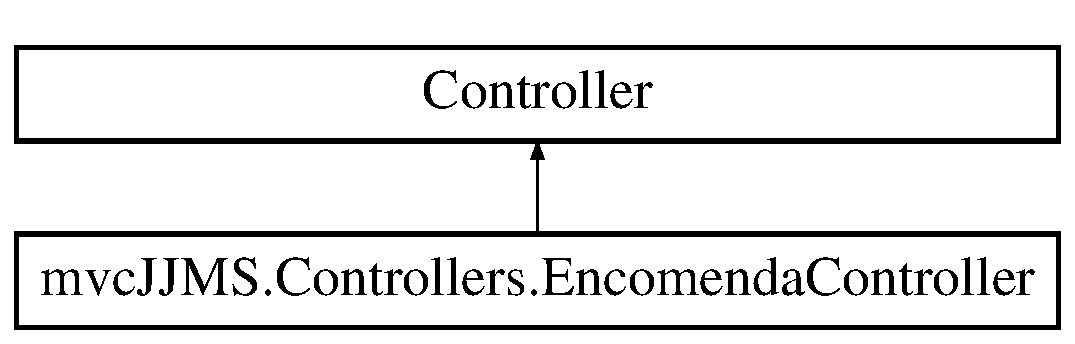
\includegraphics[height=2.000000cm]{classmvc_j_j_m_s_1_1_controllers_1_1_encomenda_controller}
\end{center}
\end{figure}
\subsection*{Public Member Functions}
\begin{DoxyCompactItemize}
\item 
\mbox{\Hypertarget{classmvc_j_j_m_s_1_1_controllers_1_1_encomenda_controller_a23ae8934385ef0e18316920583381eb2}\label{classmvc_j_j_m_s_1_1_controllers_1_1_encomenda_controller_a23ae8934385ef0e18316920583381eb2}} 
{\bfseries Encomenda\+Controller} (\mbox{\hyperlink{classmvc_j_j_m_s_1_1_data_1_1_j_j_m_s_context}{J\+J\+M\+S\+Context}} context, \mbox{\hyperlink{classmvc_j_j_m_s_1_1_controllers_1_1_fornecedor_controller}{Fornecedor\+Controller}} f\+Controller, \mbox{\hyperlink{classmvc_j_j_m_s_1_1_controllers_1_1_utilizador_controller}{Utilizador\+Controller}} u\+Controller, \mbox{\hyperlink{classmvc_j_j_m_s_1_1_controllers_1_1_cartao_controller}{Cartao\+Controller}} ca\+Controller)
\item 
Action\+Result \mbox{\hyperlink{classmvc_j_j_m_s_1_1_controllers_1_1_encomenda_controller_a4394d01a5090ea7711fc97a9d7478581}{Tracking\+Encomenda}} (int id\+Encomenda)
\item 
bool \mbox{\hyperlink{classmvc_j_j_m_s_1_1_controllers_1_1_encomenda_controller_a52ed51732bae82bd099506519656170b}{existe\+Encomenda}} (int id\+Encomenda)
\begin{DoxyCompactList}\small\item\em Checks whether there\textquotesingle{}s an order with the given identifier \end{DoxyCompactList}\item 
string \mbox{\hyperlink{classmvc_j_j_m_s_1_1_controllers_1_1_encomenda_controller_a76a4a0b0f36cb8d70f3342b601e5d8bb}{get\+Localizacao\+Encomenda}} (int id\+Encomenda)
\begin{DoxyCompactList}\small\item\em Retrieves the current location of the order \end{DoxyCompactList}\item 
int \mbox{\hyperlink{classmvc_j_j_m_s_1_1_controllers_1_1_encomenda_controller_a650422f9822c10979a38f9b7de902146}{get\+Estado\+EncomendaI}} (int id\+Encomenda)
\begin{DoxyCompactList}\small\item\em Return the current status of the order in Integer format \end{DoxyCompactList}\item 
string \mbox{\hyperlink{classmvc_j_j_m_s_1_1_controllers_1_1_encomenda_controller_a9a1c47299b334b34c9df35dd4f644184}{get\+Estado\+EncomendaS}} (int id\+Encomenda)
\begin{DoxyCompactList}\small\item\em Same as get\+Estado\+EncomendaI but returns a (descriptive) String status \end{DoxyCompactList}\item 
void \mbox{\hyperlink{classmvc_j_j_m_s_1_1_controllers_1_1_encomenda_controller_a9f2e8359f35f8d5e737c3a1d9ff7b1c1}{Update\+Custo\+Enc}} (int id\+Encomenda, float custo\+Input)
\begin{DoxyCompactList}\small\item\em Updates the cost associated with a given order \end{DoxyCompactList}\item 
void \mbox{\hyperlink{classmvc_j_j_m_s_1_1_controllers_1_1_encomenda_controller_a36abeee72b22518276b9af3d4b7ed48f}{Update\+Estado\+Enc}} (int id\+Encomenda)
\begin{DoxyCompactList}\small\item\em Changes the status of an order \end{DoxyCompactList}\item 
int \mbox{\hyperlink{classmvc_j_j_m_s_1_1_controllers_1_1_encomenda_controller_a29d51d82112bcd56e12b4c2ae5220f43}{Get\+Funcionario\+Resp}} (int id\+Encomenda)
\begin{DoxyCompactList}\small\item\em Retrieves the employee currently responsible for the order \end{DoxyCompactList}\item 
void \mbox{\hyperlink{classmvc_j_j_m_s_1_1_controllers_1_1_encomenda_controller_a88efec95120dea4ca5b3ad0e6add6abe}{Set\+Encomenda}} (int id\+Cliente, string fornecedor, string morada, Date dia, Time hora, long num\+Cart\+Credito, int mes, int ano, int cvv, string pais)
\begin{DoxyCompactList}\small\item\em Registers a new order on the database \end{DoxyCompactList}\item 
string \mbox{\hyperlink{classmvc_j_j_m_s_1_1_controllers_1_1_encomenda_controller_a17045273a7db6110840c352ccf2942f2}{Get\+Destino\+Enc}} (int id\+Encomenda)
\begin{DoxyCompactList}\small\item\em Retrieves the destination address of the order \end{DoxyCompactList}\item 
bool \mbox{\hyperlink{classmvc_j_j_m_s_1_1_controllers_1_1_encomenda_controller_a7aa095cf3c1afa66cb3b53cf58d0973d}{Encomenda\+Entregue}} (int id\+Encomenda)
\begin{DoxyCompactList}\small\item\em Checks whether an order has been delivered \end{DoxyCompactList}\item 
\mbox{\hyperlink{classmvc_j_j_m_s_1_1_models_1_1_encomenda}{Encomenda}} \mbox{\hyperlink{classmvc_j_j_m_s_1_1_controllers_1_1_encomenda_controller_adbeb0c2e410bf9d8706de7b75daf05eb}{get\+Encomenda}} (int id\+Encomenda)
\begin{DoxyCompactList}\small\item\em Retrieves the order associated with a given ID \end{DoxyCompactList}\item 
int \mbox{\hyperlink{classmvc_j_j_m_s_1_1_controllers_1_1_encomenda_controller_a27c059ba95c4c7fcd3f3c1d0d2bf51a9}{get\+Id\+Forn}} (int id\+Encomenda)
\begin{DoxyCompactList}\small\item\em Retrieves the unique identifier of the order provider \end{DoxyCompactList}\item 
string \mbox{\hyperlink{classmvc_j_j_m_s_1_1_controllers_1_1_encomenda_controller_a2754bcfc4246dcc86737356fb5ff925a}{get\+Morada\+CD}} ()
\begin{DoxyCompactList}\small\item\em Returns the Distribution Center address \end{DoxyCompactList}\item 
\mbox{\Hypertarget{classmvc_j_j_m_s_1_1_controllers_1_1_encomenda_controller_ab511489501a36b25d8211cd9ee87284b}\label{classmvc_j_j_m_s_1_1_controllers_1_1_encomenda_controller_ab511489501a36b25d8211cd9ee87284b}} 
View\+Result {\bfseries Codigo\+Inexistente} ()
\item 
\mbox{\Hypertarget{classmvc_j_j_m_s_1_1_controllers_1_1_encomenda_controller_a106850b52d6c0495216ff69b82490eee}\label{classmvc_j_j_m_s_1_1_controllers_1_1_encomenda_controller_a106850b52d6c0495216ff69b82490eee}} 
View\+Result {\bfseries Informacao\+Encomenda} (int encomenda, string localizacao, string estado)
\item 
\mbox{\Hypertarget{classmvc_j_j_m_s_1_1_controllers_1_1_encomenda_controller_a975c0c2e5081227c02fdfdb7e3e159d0}\label{classmvc_j_j_m_s_1_1_controllers_1_1_encomenda_controller_a975c0c2e5081227c02fdfdb7e3e159d0}} 
Action\+Result {\bfseries Requisitar\+Encomenda} (string fornecedor, string morada, Date dia, Time hora)
\item 
\mbox{\Hypertarget{classmvc_j_j_m_s_1_1_controllers_1_1_encomenda_controller_a9898fcedd4648f7a73d85dfc6e58ea6e}\label{classmvc_j_j_m_s_1_1_controllers_1_1_encomenda_controller_a9898fcedd4648f7a73d85dfc6e58ea6e}} 
View\+Result {\bfseries Inserir\+Dados\+Pagamento} (string fornecedor, string morada, Date dia, Time hora)
\item 
\mbox{\Hypertarget{classmvc_j_j_m_s_1_1_controllers_1_1_encomenda_controller_a5e9ff72acf751edbbace575060e434f1}\label{classmvc_j_j_m_s_1_1_controllers_1_1_encomenda_controller_a5e9ff72acf751edbbace575060e434f1}} 
View\+Result {\bfseries Proc\+Dados\+Pagamento} (string fornecedor, string morada, Date dia, Time hora, string nccS, int mes, int ano, int cvv, string pais)
\item 
\mbox{\Hypertarget{classmvc_j_j_m_s_1_1_controllers_1_1_encomenda_controller_a0ed9836d7404d96d73effb30f5bb38c0}\label{classmvc_j_j_m_s_1_1_controllers_1_1_encomenda_controller_a0ed9836d7404d96d73effb30f5bb38c0}} 
View\+Result {\bfseries Dados\+Pagamento\+Invalidos} ()
\item 
\mbox{\Hypertarget{classmvc_j_j_m_s_1_1_controllers_1_1_encomenda_controller_af1ffc3ade26ffaeb8a51456d7f4af930}\label{classmvc_j_j_m_s_1_1_controllers_1_1_encomenda_controller_af1ffc3ade26ffaeb8a51456d7f4af930}} 
View\+Result {\bfseries Fornecedor\+Invalido} ()
\item 
\mbox{\Hypertarget{classmvc_j_j_m_s_1_1_controllers_1_1_encomenda_controller_ab027738b2e4dfce7c7f19c6cf13cf078}\label{classmvc_j_j_m_s_1_1_controllers_1_1_encomenda_controller_ab027738b2e4dfce7c7f19c6cf13cf078}} 
View\+Result {\bfseries Sucesso} ()
\end{DoxyCompactItemize}


\subsection{Member Function Documentation}
\mbox{\Hypertarget{classmvc_j_j_m_s_1_1_controllers_1_1_encomenda_controller_a7aa095cf3c1afa66cb3b53cf58d0973d}\label{classmvc_j_j_m_s_1_1_controllers_1_1_encomenda_controller_a7aa095cf3c1afa66cb3b53cf58d0973d}} 
\index{mvc\+J\+J\+M\+S\+::\+Controllers\+::\+Encomenda\+Controller@{mvc\+J\+J\+M\+S\+::\+Controllers\+::\+Encomenda\+Controller}!Encomenda\+Entregue@{Encomenda\+Entregue}}
\index{Encomenda\+Entregue@{Encomenda\+Entregue}!mvc\+J\+J\+M\+S\+::\+Controllers\+::\+Encomenda\+Controller@{mvc\+J\+J\+M\+S\+::\+Controllers\+::\+Encomenda\+Controller}}
\subsubsection{\texorpdfstring{Encomenda\+Entregue()}{EncomendaEntregue()}}
{\footnotesize\ttfamily bool mvc\+J\+J\+M\+S.\+Controllers.\+Encomenda\+Controller.\+Encomenda\+Entregue (\begin{DoxyParamCaption}\item[{int}]{id\+Encomenda }\end{DoxyParamCaption})\hspace{0.3cm}{\ttfamily [inline]}}



Checks whether an order has been delivered 


\begin{DoxyParams}{Parameters}
{\em id\+Encomenda} & Unique identifier for a single order\\
\hline
\end{DoxyParams}
\begin{DoxyReturn}{Returns}
T\+R\+UE if delivered else F\+A\+L\+SE
\end{DoxyReturn}
\mbox{\Hypertarget{classmvc_j_j_m_s_1_1_controllers_1_1_encomenda_controller_a52ed51732bae82bd099506519656170b}\label{classmvc_j_j_m_s_1_1_controllers_1_1_encomenda_controller_a52ed51732bae82bd099506519656170b}} 
\index{mvc\+J\+J\+M\+S\+::\+Controllers\+::\+Encomenda\+Controller@{mvc\+J\+J\+M\+S\+::\+Controllers\+::\+Encomenda\+Controller}!existe\+Encomenda@{existe\+Encomenda}}
\index{existe\+Encomenda@{existe\+Encomenda}!mvc\+J\+J\+M\+S\+::\+Controllers\+::\+Encomenda\+Controller@{mvc\+J\+J\+M\+S\+::\+Controllers\+::\+Encomenda\+Controller}}
\subsubsection{\texorpdfstring{existe\+Encomenda()}{existeEncomenda()}}
{\footnotesize\ttfamily bool mvc\+J\+J\+M\+S.\+Controllers.\+Encomenda\+Controller.\+existe\+Encomenda (\begin{DoxyParamCaption}\item[{int}]{id\+Encomenda }\end{DoxyParamCaption})\hspace{0.3cm}{\ttfamily [inline]}}



Checks whether there\textquotesingle{}s an order with the given identifier 


\begin{DoxyParams}{Parameters}
{\em id\+Encomenda} & Unique identifier for a single order\\
\hline
\end{DoxyParams}
\begin{DoxyReturn}{Returns}
T\+R\+UE if there is an order with the identifier else F\+A\+L\+SE
\end{DoxyReturn}
\mbox{\Hypertarget{classmvc_j_j_m_s_1_1_controllers_1_1_encomenda_controller_a17045273a7db6110840c352ccf2942f2}\label{classmvc_j_j_m_s_1_1_controllers_1_1_encomenda_controller_a17045273a7db6110840c352ccf2942f2}} 
\index{mvc\+J\+J\+M\+S\+::\+Controllers\+::\+Encomenda\+Controller@{mvc\+J\+J\+M\+S\+::\+Controllers\+::\+Encomenda\+Controller}!Get\+Destino\+Enc@{Get\+Destino\+Enc}}
\index{Get\+Destino\+Enc@{Get\+Destino\+Enc}!mvc\+J\+J\+M\+S\+::\+Controllers\+::\+Encomenda\+Controller@{mvc\+J\+J\+M\+S\+::\+Controllers\+::\+Encomenda\+Controller}}
\subsubsection{\texorpdfstring{Get\+Destino\+Enc()}{GetDestinoEnc()}}
{\footnotesize\ttfamily string mvc\+J\+J\+M\+S.\+Controllers.\+Encomenda\+Controller.\+Get\+Destino\+Enc (\begin{DoxyParamCaption}\item[{int}]{id\+Encomenda }\end{DoxyParamCaption})\hspace{0.3cm}{\ttfamily [inline]}}



Retrieves the destination address of the order 


\begin{DoxyParams}{Parameters}
{\em id\+Encomenda} & Unique identifier for a single order\\
\hline
\end{DoxyParams}
\begin{DoxyReturn}{Returns}
Destination address
\end{DoxyReturn}
\mbox{\Hypertarget{classmvc_j_j_m_s_1_1_controllers_1_1_encomenda_controller_adbeb0c2e410bf9d8706de7b75daf05eb}\label{classmvc_j_j_m_s_1_1_controllers_1_1_encomenda_controller_adbeb0c2e410bf9d8706de7b75daf05eb}} 
\index{mvc\+J\+J\+M\+S\+::\+Controllers\+::\+Encomenda\+Controller@{mvc\+J\+J\+M\+S\+::\+Controllers\+::\+Encomenda\+Controller}!get\+Encomenda@{get\+Encomenda}}
\index{get\+Encomenda@{get\+Encomenda}!mvc\+J\+J\+M\+S\+::\+Controllers\+::\+Encomenda\+Controller@{mvc\+J\+J\+M\+S\+::\+Controllers\+::\+Encomenda\+Controller}}
\subsubsection{\texorpdfstring{get\+Encomenda()}{getEncomenda()}}
{\footnotesize\ttfamily \mbox{\hyperlink{classmvc_j_j_m_s_1_1_models_1_1_encomenda}{Encomenda}} mvc\+J\+J\+M\+S.\+Controllers.\+Encomenda\+Controller.\+get\+Encomenda (\begin{DoxyParamCaption}\item[{int}]{id\+Encomenda }\end{DoxyParamCaption})\hspace{0.3cm}{\ttfamily [inline]}}



Retrieves the order associated with a given ID 


\begin{DoxyParams}{Parameters}
{\em id\+Encomenda} & Unique identifier for a single order\\
\hline
\end{DoxyParams}
\begin{DoxyReturn}{Returns}
Order corresponding to the ID
\end{DoxyReturn}
\mbox{\Hypertarget{classmvc_j_j_m_s_1_1_controllers_1_1_encomenda_controller_a650422f9822c10979a38f9b7de902146}\label{classmvc_j_j_m_s_1_1_controllers_1_1_encomenda_controller_a650422f9822c10979a38f9b7de902146}} 
\index{mvc\+J\+J\+M\+S\+::\+Controllers\+::\+Encomenda\+Controller@{mvc\+J\+J\+M\+S\+::\+Controllers\+::\+Encomenda\+Controller}!get\+Estado\+EncomendaI@{get\+Estado\+EncomendaI}}
\index{get\+Estado\+EncomendaI@{get\+Estado\+EncomendaI}!mvc\+J\+J\+M\+S\+::\+Controllers\+::\+Encomenda\+Controller@{mvc\+J\+J\+M\+S\+::\+Controllers\+::\+Encomenda\+Controller}}
\subsubsection{\texorpdfstring{get\+Estado\+Encomenda\+I()}{getEstadoEncomendaI()}}
{\footnotesize\ttfamily int mvc\+J\+J\+M\+S.\+Controllers.\+Encomenda\+Controller.\+get\+Estado\+EncomendaI (\begin{DoxyParamCaption}\item[{int}]{id\+Encomenda }\end{DoxyParamCaption})\hspace{0.3cm}{\ttfamily [inline]}}



Return the current status of the order in Integer format 


\begin{DoxyParams}{Parameters}
{\em id\+Encomenda} & Unique identifier for a single order\\
\hline
\end{DoxyParams}
\begin{DoxyReturn}{Returns}

\end{DoxyReturn}
\mbox{\Hypertarget{classmvc_j_j_m_s_1_1_controllers_1_1_encomenda_controller_a9a1c47299b334b34c9df35dd4f644184}\label{classmvc_j_j_m_s_1_1_controllers_1_1_encomenda_controller_a9a1c47299b334b34c9df35dd4f644184}} 
\index{mvc\+J\+J\+M\+S\+::\+Controllers\+::\+Encomenda\+Controller@{mvc\+J\+J\+M\+S\+::\+Controllers\+::\+Encomenda\+Controller}!get\+Estado\+EncomendaS@{get\+Estado\+EncomendaS}}
\index{get\+Estado\+EncomendaS@{get\+Estado\+EncomendaS}!mvc\+J\+J\+M\+S\+::\+Controllers\+::\+Encomenda\+Controller@{mvc\+J\+J\+M\+S\+::\+Controllers\+::\+Encomenda\+Controller}}
\subsubsection{\texorpdfstring{get\+Estado\+Encomenda\+S()}{getEstadoEncomendaS()}}
{\footnotesize\ttfamily string mvc\+J\+J\+M\+S.\+Controllers.\+Encomenda\+Controller.\+get\+Estado\+EncomendaS (\begin{DoxyParamCaption}\item[{int}]{id\+Encomenda }\end{DoxyParamCaption})\hspace{0.3cm}{\ttfamily [inline]}}



Same as get\+Estado\+EncomendaI but returns a (descriptive) String status 


\begin{DoxyParams}{Parameters}
{\em id\+Encomenda} & Unique identifier for a single order\\
\hline
\end{DoxyParams}
\begin{DoxyReturn}{Returns}

\end{DoxyReturn}
\mbox{\Hypertarget{classmvc_j_j_m_s_1_1_controllers_1_1_encomenda_controller_a29d51d82112bcd56e12b4c2ae5220f43}\label{classmvc_j_j_m_s_1_1_controllers_1_1_encomenda_controller_a29d51d82112bcd56e12b4c2ae5220f43}} 
\index{mvc\+J\+J\+M\+S\+::\+Controllers\+::\+Encomenda\+Controller@{mvc\+J\+J\+M\+S\+::\+Controllers\+::\+Encomenda\+Controller}!Get\+Funcionario\+Resp@{Get\+Funcionario\+Resp}}
\index{Get\+Funcionario\+Resp@{Get\+Funcionario\+Resp}!mvc\+J\+J\+M\+S\+::\+Controllers\+::\+Encomenda\+Controller@{mvc\+J\+J\+M\+S\+::\+Controllers\+::\+Encomenda\+Controller}}
\subsubsection{\texorpdfstring{Get\+Funcionario\+Resp()}{GetFuncionarioResp()}}
{\footnotesize\ttfamily int mvc\+J\+J\+M\+S.\+Controllers.\+Encomenda\+Controller.\+Get\+Funcionario\+Resp (\begin{DoxyParamCaption}\item[{int}]{id\+Encomenda }\end{DoxyParamCaption})\hspace{0.3cm}{\ttfamily [inline]}}



Retrieves the employee currently responsible for the order 


\begin{DoxyParams}{Parameters}
{\em id\+Encomenda} & Unique identifier for a single order\\
\hline
\end{DoxyParams}
\begin{DoxyReturn}{Returns}
Unique identifier of the employee
\end{DoxyReturn}
\mbox{\Hypertarget{classmvc_j_j_m_s_1_1_controllers_1_1_encomenda_controller_a27c059ba95c4c7fcd3f3c1d0d2bf51a9}\label{classmvc_j_j_m_s_1_1_controllers_1_1_encomenda_controller_a27c059ba95c4c7fcd3f3c1d0d2bf51a9}} 
\index{mvc\+J\+J\+M\+S\+::\+Controllers\+::\+Encomenda\+Controller@{mvc\+J\+J\+M\+S\+::\+Controllers\+::\+Encomenda\+Controller}!get\+Id\+Forn@{get\+Id\+Forn}}
\index{get\+Id\+Forn@{get\+Id\+Forn}!mvc\+J\+J\+M\+S\+::\+Controllers\+::\+Encomenda\+Controller@{mvc\+J\+J\+M\+S\+::\+Controllers\+::\+Encomenda\+Controller}}
\subsubsection{\texorpdfstring{get\+Id\+Forn()}{getIdForn()}}
{\footnotesize\ttfamily int mvc\+J\+J\+M\+S.\+Controllers.\+Encomenda\+Controller.\+get\+Id\+Forn (\begin{DoxyParamCaption}\item[{int}]{id\+Encomenda }\end{DoxyParamCaption})\hspace{0.3cm}{\ttfamily [inline]}}



Retrieves the unique identifier of the order provider 


\begin{DoxyParams}{Parameters}
{\em id\+Encomenda} & Unique identifier for a single order\\
\hline
\end{DoxyParams}
\begin{DoxyReturn}{Returns}
Unique identifier of the order provider
\end{DoxyReturn}
\mbox{\Hypertarget{classmvc_j_j_m_s_1_1_controllers_1_1_encomenda_controller_a76a4a0b0f36cb8d70f3342b601e5d8bb}\label{classmvc_j_j_m_s_1_1_controllers_1_1_encomenda_controller_a76a4a0b0f36cb8d70f3342b601e5d8bb}} 
\index{mvc\+J\+J\+M\+S\+::\+Controllers\+::\+Encomenda\+Controller@{mvc\+J\+J\+M\+S\+::\+Controllers\+::\+Encomenda\+Controller}!get\+Localizacao\+Encomenda@{get\+Localizacao\+Encomenda}}
\index{get\+Localizacao\+Encomenda@{get\+Localizacao\+Encomenda}!mvc\+J\+J\+M\+S\+::\+Controllers\+::\+Encomenda\+Controller@{mvc\+J\+J\+M\+S\+::\+Controllers\+::\+Encomenda\+Controller}}
\subsubsection{\texorpdfstring{get\+Localizacao\+Encomenda()}{getLocalizacaoEncomenda()}}
{\footnotesize\ttfamily string mvc\+J\+J\+M\+S.\+Controllers.\+Encomenda\+Controller.\+get\+Localizacao\+Encomenda (\begin{DoxyParamCaption}\item[{int}]{id\+Encomenda }\end{DoxyParamCaption})\hspace{0.3cm}{\ttfamily [inline]}}



Retrieves the current location of the order 


\begin{DoxyParams}{Parameters}
{\em id\+Encomenda} & Unique identifier for a single order\\
\hline
\end{DoxyParams}
\begin{DoxyReturn}{Returns}
Current location of the order
\end{DoxyReturn}
\mbox{\Hypertarget{classmvc_j_j_m_s_1_1_controllers_1_1_encomenda_controller_a2754bcfc4246dcc86737356fb5ff925a}\label{classmvc_j_j_m_s_1_1_controllers_1_1_encomenda_controller_a2754bcfc4246dcc86737356fb5ff925a}} 
\index{mvc\+J\+J\+M\+S\+::\+Controllers\+::\+Encomenda\+Controller@{mvc\+J\+J\+M\+S\+::\+Controllers\+::\+Encomenda\+Controller}!get\+Morada\+CD@{get\+Morada\+CD}}
\index{get\+Morada\+CD@{get\+Morada\+CD}!mvc\+J\+J\+M\+S\+::\+Controllers\+::\+Encomenda\+Controller@{mvc\+J\+J\+M\+S\+::\+Controllers\+::\+Encomenda\+Controller}}
\subsubsection{\texorpdfstring{get\+Morada\+C\+D()}{getMoradaCD()}}
{\footnotesize\ttfamily string mvc\+J\+J\+M\+S.\+Controllers.\+Encomenda\+Controller.\+get\+Morada\+CD (\begin{DoxyParamCaption}{ }\end{DoxyParamCaption})\hspace{0.3cm}{\ttfamily [inline]}}



Returns the Distribution Center address 

\begin{DoxyReturn}{Returns}
Distribuition Center address
\end{DoxyReturn}
\mbox{\Hypertarget{classmvc_j_j_m_s_1_1_controllers_1_1_encomenda_controller_a88efec95120dea4ca5b3ad0e6add6abe}\label{classmvc_j_j_m_s_1_1_controllers_1_1_encomenda_controller_a88efec95120dea4ca5b3ad0e6add6abe}} 
\index{mvc\+J\+J\+M\+S\+::\+Controllers\+::\+Encomenda\+Controller@{mvc\+J\+J\+M\+S\+::\+Controllers\+::\+Encomenda\+Controller}!Set\+Encomenda@{Set\+Encomenda}}
\index{Set\+Encomenda@{Set\+Encomenda}!mvc\+J\+J\+M\+S\+::\+Controllers\+::\+Encomenda\+Controller@{mvc\+J\+J\+M\+S\+::\+Controllers\+::\+Encomenda\+Controller}}
\subsubsection{\texorpdfstring{Set\+Encomenda()}{SetEncomenda()}}
{\footnotesize\ttfamily void mvc\+J\+J\+M\+S.\+Controllers.\+Encomenda\+Controller.\+Set\+Encomenda (\begin{DoxyParamCaption}\item[{int}]{id\+Cliente,  }\item[{string}]{fornecedor,  }\item[{string}]{morada,  }\item[{Date}]{dia,  }\item[{Time}]{hora,  }\item[{long}]{num\+Cart\+Credito,  }\item[{int}]{mes,  }\item[{int}]{ano,  }\item[{int}]{cvv,  }\item[{string}]{pais }\end{DoxyParamCaption})\hspace{0.3cm}{\ttfamily [inline]}}



Registers a new order on the database 


\begin{DoxyParams}{Parameters}
{\em id\+Cliente} & Unique identifier of the client\\
\hline
{\em fornecedor} & \\
\hline
{\em morada} & Destination of the order\\
\hline
{\em dia} & Day of delivery\\
\hline
{\em hora} & Time of delivery\\
\hline
{\em num\+Cart\+Credito} & Credit card number for payment\\
\hline
{\em mes} & Month of expiration of the credit card\\
\hline
{\em ano} & Year of expiration of the credit card\\
\hline
{\em cvv} & Security code of credit card\\
\hline
{\em pais} & Country of credit card\\
\hline
\end{DoxyParams}
\mbox{\Hypertarget{classmvc_j_j_m_s_1_1_controllers_1_1_encomenda_controller_a4394d01a5090ea7711fc97a9d7478581}\label{classmvc_j_j_m_s_1_1_controllers_1_1_encomenda_controller_a4394d01a5090ea7711fc97a9d7478581}} 
\index{mvc\+J\+J\+M\+S\+::\+Controllers\+::\+Encomenda\+Controller@{mvc\+J\+J\+M\+S\+::\+Controllers\+::\+Encomenda\+Controller}!Tracking\+Encomenda@{Tracking\+Encomenda}}
\index{Tracking\+Encomenda@{Tracking\+Encomenda}!mvc\+J\+J\+M\+S\+::\+Controllers\+::\+Encomenda\+Controller@{mvc\+J\+J\+M\+S\+::\+Controllers\+::\+Encomenda\+Controller}}
\subsubsection{\texorpdfstring{Tracking\+Encomenda()}{TrackingEncomenda()}}
{\footnotesize\ttfamily Action\+Result mvc\+J\+J\+M\+S.\+Controllers.\+Encomenda\+Controller.\+Tracking\+Encomenda (\begin{DoxyParamCaption}\item[{int}]{id\+Encomenda }\end{DoxyParamCaption})\hspace{0.3cm}{\ttfamily [inline]}}






\begin{DoxyParams}{Parameters}
{\em id\+Encomenda} & \\
\hline
\end{DoxyParams}
\begin{DoxyReturn}{Returns}

\end{DoxyReturn}
\mbox{\Hypertarget{classmvc_j_j_m_s_1_1_controllers_1_1_encomenda_controller_a9f2e8359f35f8d5e737c3a1d9ff7b1c1}\label{classmvc_j_j_m_s_1_1_controllers_1_1_encomenda_controller_a9f2e8359f35f8d5e737c3a1d9ff7b1c1}} 
\index{mvc\+J\+J\+M\+S\+::\+Controllers\+::\+Encomenda\+Controller@{mvc\+J\+J\+M\+S\+::\+Controllers\+::\+Encomenda\+Controller}!Update\+Custo\+Enc@{Update\+Custo\+Enc}}
\index{Update\+Custo\+Enc@{Update\+Custo\+Enc}!mvc\+J\+J\+M\+S\+::\+Controllers\+::\+Encomenda\+Controller@{mvc\+J\+J\+M\+S\+::\+Controllers\+::\+Encomenda\+Controller}}
\subsubsection{\texorpdfstring{Update\+Custo\+Enc()}{UpdateCustoEnc()}}
{\footnotesize\ttfamily void mvc\+J\+J\+M\+S.\+Controllers.\+Encomenda\+Controller.\+Update\+Custo\+Enc (\begin{DoxyParamCaption}\item[{int}]{id\+Encomenda,  }\item[{float}]{custo\+Input }\end{DoxyParamCaption})\hspace{0.3cm}{\ttfamily [inline]}}



Updates the cost associated with a given order 


\begin{DoxyParams}{Parameters}
{\em id\+Encomenda} & Unique identifier for a single order\\
\hline
{\em custo\+Input} & Cost of the order\\
\hline
\end{DoxyParams}
\mbox{\Hypertarget{classmvc_j_j_m_s_1_1_controllers_1_1_encomenda_controller_a36abeee72b22518276b9af3d4b7ed48f}\label{classmvc_j_j_m_s_1_1_controllers_1_1_encomenda_controller_a36abeee72b22518276b9af3d4b7ed48f}} 
\index{mvc\+J\+J\+M\+S\+::\+Controllers\+::\+Encomenda\+Controller@{mvc\+J\+J\+M\+S\+::\+Controllers\+::\+Encomenda\+Controller}!Update\+Estado\+Enc@{Update\+Estado\+Enc}}
\index{Update\+Estado\+Enc@{Update\+Estado\+Enc}!mvc\+J\+J\+M\+S\+::\+Controllers\+::\+Encomenda\+Controller@{mvc\+J\+J\+M\+S\+::\+Controllers\+::\+Encomenda\+Controller}}
\subsubsection{\texorpdfstring{Update\+Estado\+Enc()}{UpdateEstadoEnc()}}
{\footnotesize\ttfamily void mvc\+J\+J\+M\+S.\+Controllers.\+Encomenda\+Controller.\+Update\+Estado\+Enc (\begin{DoxyParamCaption}\item[{int}]{id\+Encomenda }\end{DoxyParamCaption})\hspace{0.3cm}{\ttfamily [inline]}}



Changes the status of an order 


\begin{DoxyParams}{Parameters}
{\em id\+Encomenda} & Unique identifier for a single order\\
\hline
\end{DoxyParams}


The documentation for this class was generated from the following file\+:\begin{DoxyCompactItemize}
\item 
Controllers/Encomenda\+Controller.\+cs\end{DoxyCompactItemize}

\hypertarget{classmvc_j_j_m_s_1_1_models_1_1_fornecedor}{}\section{mvc\+J\+J\+M\+S.\+Models.\+Fornecedor Class Reference}
\label{classmvc_j_j_m_s_1_1_models_1_1_fornecedor}\index{mvc\+J\+J\+M\+S.\+Models.\+Fornecedor@{mvc\+J\+J\+M\+S.\+Models.\+Fornecedor}}


Represents a provider from which Clients can order products  


\subsection*{Public Member Functions}
\begin{DoxyCompactItemize}
\item 
void \mbox{\hyperlink{classmvc_j_j_m_s_1_1_models_1_1_fornecedor_a6197573e85fd7091904f00eda7444bc3}{set\+Nome}} (string nome)
\begin{DoxyCompactList}\small\item\em set the name of Fornecedor(provider) \end{DoxyCompactList}\item 
void \mbox{\hyperlink{classmvc_j_j_m_s_1_1_models_1_1_fornecedor_a8a3919c2983ee05ac36144ef604a9264}{set\+Morada}} (string morada)
\begin{DoxyCompactList}\small\item\em set the adress of Fornecedor(provider) \end{DoxyCompactList}\item 
string \mbox{\hyperlink{classmvc_j_j_m_s_1_1_models_1_1_fornecedor_adbbebab32a2d6ba5cb4f14c3089b9373}{get\+Nome}} ()
\begin{DoxyCompactList}\small\item\em obtain the name of Fornecedor(provider) \end{DoxyCompactList}\end{DoxyCompactItemize}
\subsection*{Properties}
\begin{DoxyCompactItemize}
\item 
\mbox{\Hypertarget{classmvc_j_j_m_s_1_1_models_1_1_fornecedor_a2a58cfd29948857208d37d5b40b864a4}\label{classmvc_j_j_m_s_1_1_models_1_1_fornecedor_a2a58cfd29948857208d37d5b40b864a4}} 
int {\bfseries Fornecedor\+ID}\hspace{0.3cm}{\ttfamily  \mbox{[}get, set\mbox{]}}
\item 
\mbox{\Hypertarget{classmvc_j_j_m_s_1_1_models_1_1_fornecedor_a5455734cda3c1e95a1a758c26020bbfe}\label{classmvc_j_j_m_s_1_1_models_1_1_fornecedor_a5455734cda3c1e95a1a758c26020bbfe}} 
string {\bfseries nome}\hspace{0.3cm}{\ttfamily  \mbox{[}get, set\mbox{]}}
\item 
\mbox{\Hypertarget{classmvc_j_j_m_s_1_1_models_1_1_fornecedor_a05208e05a32384b3d6b29f9c2172047d}\label{classmvc_j_j_m_s_1_1_models_1_1_fornecedor_a05208e05a32384b3d6b29f9c2172047d}} 
string {\bfseries morada}\hspace{0.3cm}{\ttfamily  \mbox{[}get, set\mbox{]}}
\item 
\mbox{\Hypertarget{classmvc_j_j_m_s_1_1_models_1_1_fornecedor_a7dd659939d00a56e77608c477eff18e9}\label{classmvc_j_j_m_s_1_1_models_1_1_fornecedor_a7dd659939d00a56e77608c477eff18e9}} 
I\+Collection$<$ \mbox{\hyperlink{classmvc_j_j_m_s_1_1_models_1_1_encomenda}{Encomenda}} $>$ {\bfseries Encomendas}\hspace{0.3cm}{\ttfamily  \mbox{[}get, set\mbox{]}}
\end{DoxyCompactItemize}


\subsection{Detailed Description}
Represents a provider from which Clients can order products 



\subsection{Member Function Documentation}
\mbox{\Hypertarget{classmvc_j_j_m_s_1_1_models_1_1_fornecedor_adbbebab32a2d6ba5cb4f14c3089b9373}\label{classmvc_j_j_m_s_1_1_models_1_1_fornecedor_adbbebab32a2d6ba5cb4f14c3089b9373}} 
\index{mvc\+J\+J\+M\+S\+::\+Models\+::\+Fornecedor@{mvc\+J\+J\+M\+S\+::\+Models\+::\+Fornecedor}!get\+Nome@{get\+Nome}}
\index{get\+Nome@{get\+Nome}!mvc\+J\+J\+M\+S\+::\+Models\+::\+Fornecedor@{mvc\+J\+J\+M\+S\+::\+Models\+::\+Fornecedor}}
\subsubsection{\texorpdfstring{get\+Nome()}{getNome()}}
{\footnotesize\ttfamily string mvc\+J\+J\+M\+S.\+Models.\+Fornecedor.\+get\+Nome (\begin{DoxyParamCaption}{ }\end{DoxyParamCaption})\hspace{0.3cm}{\ttfamily [inline]}}



obtain the name of Fornecedor(provider) 

\begin{DoxyReturn}{Returns}
return the name
\end{DoxyReturn}
\mbox{\Hypertarget{classmvc_j_j_m_s_1_1_models_1_1_fornecedor_a8a3919c2983ee05ac36144ef604a9264}\label{classmvc_j_j_m_s_1_1_models_1_1_fornecedor_a8a3919c2983ee05ac36144ef604a9264}} 
\index{mvc\+J\+J\+M\+S\+::\+Models\+::\+Fornecedor@{mvc\+J\+J\+M\+S\+::\+Models\+::\+Fornecedor}!set\+Morada@{set\+Morada}}
\index{set\+Morada@{set\+Morada}!mvc\+J\+J\+M\+S\+::\+Models\+::\+Fornecedor@{mvc\+J\+J\+M\+S\+::\+Models\+::\+Fornecedor}}
\subsubsection{\texorpdfstring{set\+Morada()}{setMorada()}}
{\footnotesize\ttfamily void mvc\+J\+J\+M\+S.\+Models.\+Fornecedor.\+set\+Morada (\begin{DoxyParamCaption}\item[{string}]{morada }\end{DoxyParamCaption})\hspace{0.3cm}{\ttfamily [inline]}}



set the adress of Fornecedor(provider) 


\begin{DoxyParams}{Parameters}
{\em morada} & \\
\hline
\end{DoxyParams}
\mbox{\Hypertarget{classmvc_j_j_m_s_1_1_models_1_1_fornecedor_a6197573e85fd7091904f00eda7444bc3}\label{classmvc_j_j_m_s_1_1_models_1_1_fornecedor_a6197573e85fd7091904f00eda7444bc3}} 
\index{mvc\+J\+J\+M\+S\+::\+Models\+::\+Fornecedor@{mvc\+J\+J\+M\+S\+::\+Models\+::\+Fornecedor}!set\+Nome@{set\+Nome}}
\index{set\+Nome@{set\+Nome}!mvc\+J\+J\+M\+S\+::\+Models\+::\+Fornecedor@{mvc\+J\+J\+M\+S\+::\+Models\+::\+Fornecedor}}
\subsubsection{\texorpdfstring{set\+Nome()}{setNome()}}
{\footnotesize\ttfamily void mvc\+J\+J\+M\+S.\+Models.\+Fornecedor.\+set\+Nome (\begin{DoxyParamCaption}\item[{string}]{nome }\end{DoxyParamCaption})\hspace{0.3cm}{\ttfamily [inline]}}



set the name of Fornecedor(provider) 


\begin{DoxyParams}{Parameters}
{\em nome} & \\
\hline
\end{DoxyParams}


The documentation for this class was generated from the following file\+:\begin{DoxyCompactItemize}
\item 
Models/Fornecedor.\+cs\end{DoxyCompactItemize}

\hypertarget{classmvc_j_j_m_s_1_1_controllers_1_1_fornecedor_controller}{}\section{mvc\+J\+J\+M\+S.\+Controllers.\+Fornecedor\+Controller Class Reference}
\label{classmvc_j_j_m_s_1_1_controllers_1_1_fornecedor_controller}\index{mvc\+J\+J\+M\+S.\+Controllers.\+Fornecedor\+Controller@{mvc\+J\+J\+M\+S.\+Controllers.\+Fornecedor\+Controller}}
Inheritance diagram for mvc\+J\+J\+M\+S.\+Controllers.\+Fornecedor\+Controller\+:\begin{figure}[H]
\begin{center}
\leavevmode
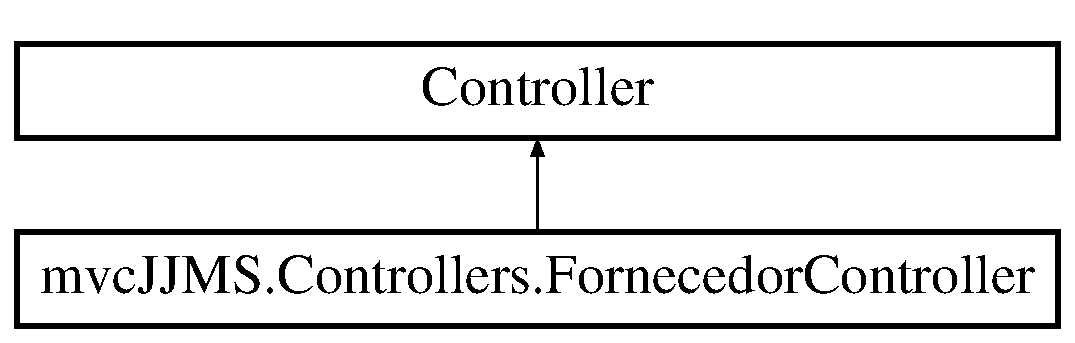
\includegraphics[height=2.000000cm]{classmvc_j_j_m_s_1_1_controllers_1_1_fornecedor_controller}
\end{center}
\end{figure}
\subsection*{Public Member Functions}
\begin{DoxyCompactItemize}
\item 
\mbox{\Hypertarget{classmvc_j_j_m_s_1_1_controllers_1_1_fornecedor_controller_ad52283ae0d089a077433d7427fbe18f6}\label{classmvc_j_j_m_s_1_1_controllers_1_1_fornecedor_controller_ad52283ae0d089a077433d7427fbe18f6}} 
{\bfseries Fornecedor\+Controller} (\mbox{\hyperlink{classmvc_j_j_m_s_1_1_data_1_1_j_j_m_s_context}{J\+J\+M\+S\+Context}} context)
\item 
int \mbox{\hyperlink{classmvc_j_j_m_s_1_1_controllers_1_1_fornecedor_controller_aff86c90ff49596167a21019cc0666de9}{Id\+Forn}} (string nome\+Forn)
\begin{DoxyCompactList}\small\item\em obtain the id of Fornecedor with nome\+Forn \end{DoxyCompactList}\item 
string \mbox{\hyperlink{classmvc_j_j_m_s_1_1_controllers_1_1_fornecedor_controller_a2f7a5b563e072a228f1b9fe5da68afb4}{Get\+Morada\+Forn}} (int id\+Forn)
\begin{DoxyCompactList}\small\item\em obtains adress of Fornecedor with the id id\+Forn \end{DoxyCompactList}\end{DoxyCompactItemize}


\subsection{Member Function Documentation}
\mbox{\Hypertarget{classmvc_j_j_m_s_1_1_controllers_1_1_fornecedor_controller_a2f7a5b563e072a228f1b9fe5da68afb4}\label{classmvc_j_j_m_s_1_1_controllers_1_1_fornecedor_controller_a2f7a5b563e072a228f1b9fe5da68afb4}} 
\index{mvc\+J\+J\+M\+S\+::\+Controllers\+::\+Fornecedor\+Controller@{mvc\+J\+J\+M\+S\+::\+Controllers\+::\+Fornecedor\+Controller}!Get\+Morada\+Forn@{Get\+Morada\+Forn}}
\index{Get\+Morada\+Forn@{Get\+Morada\+Forn}!mvc\+J\+J\+M\+S\+::\+Controllers\+::\+Fornecedor\+Controller@{mvc\+J\+J\+M\+S\+::\+Controllers\+::\+Fornecedor\+Controller}}
\subsubsection{\texorpdfstring{Get\+Morada\+Forn()}{GetMoradaForn()}}
{\footnotesize\ttfamily string mvc\+J\+J\+M\+S.\+Controllers.\+Fornecedor\+Controller.\+Get\+Morada\+Forn (\begin{DoxyParamCaption}\item[{int}]{id\+Forn }\end{DoxyParamCaption})\hspace{0.3cm}{\ttfamily [inline]}}



obtains adress of Fornecedor with the id id\+Forn 


\begin{DoxyParams}{Parameters}
{\em id\+Forn} & \\
\hline
\end{DoxyParams}
\begin{DoxyReturn}{Returns}
returns adress of Fornecedor
\end{DoxyReturn}
\mbox{\Hypertarget{classmvc_j_j_m_s_1_1_controllers_1_1_fornecedor_controller_aff86c90ff49596167a21019cc0666de9}\label{classmvc_j_j_m_s_1_1_controllers_1_1_fornecedor_controller_aff86c90ff49596167a21019cc0666de9}} 
\index{mvc\+J\+J\+M\+S\+::\+Controllers\+::\+Fornecedor\+Controller@{mvc\+J\+J\+M\+S\+::\+Controllers\+::\+Fornecedor\+Controller}!Id\+Forn@{Id\+Forn}}
\index{Id\+Forn@{Id\+Forn}!mvc\+J\+J\+M\+S\+::\+Controllers\+::\+Fornecedor\+Controller@{mvc\+J\+J\+M\+S\+::\+Controllers\+::\+Fornecedor\+Controller}}
\subsubsection{\texorpdfstring{Id\+Forn()}{IdForn()}}
{\footnotesize\ttfamily int mvc\+J\+J\+M\+S.\+Controllers.\+Fornecedor\+Controller.\+Id\+Forn (\begin{DoxyParamCaption}\item[{string}]{nome\+Forn }\end{DoxyParamCaption})\hspace{0.3cm}{\ttfamily [inline]}}



obtain the id of Fornecedor with nome\+Forn 


\begin{DoxyParams}{Parameters}
{\em nome\+Forn} & \\
\hline
\end{DoxyParams}
\begin{DoxyReturn}{Returns}
returns id of Fornecedor or -\/1 if not exists
\end{DoxyReturn}


The documentation for this class was generated from the following file\+:\begin{DoxyCompactItemize}
\item 
Controllers/Fornecedor\+Controller.\+cs\end{DoxyCompactItemize}

\hypertarget{classmvc_j_j_m_s_1_1_models_1_1_funcionario}{}\section{mvc\+J\+J\+M\+S.\+Models.\+Funcionario Class Reference}
\label{classmvc_j_j_m_s_1_1_models_1_1_funcionario}\index{mvc\+J\+J\+M\+S.\+Models.\+Funcionario@{mvc\+J\+J\+M\+S.\+Models.\+Funcionario}}


Represents a user of type employee  


Inheritance diagram for mvc\+J\+J\+M\+S.\+Models.\+Funcionario\+:\begin{figure}[H]
\begin{center}
\leavevmode
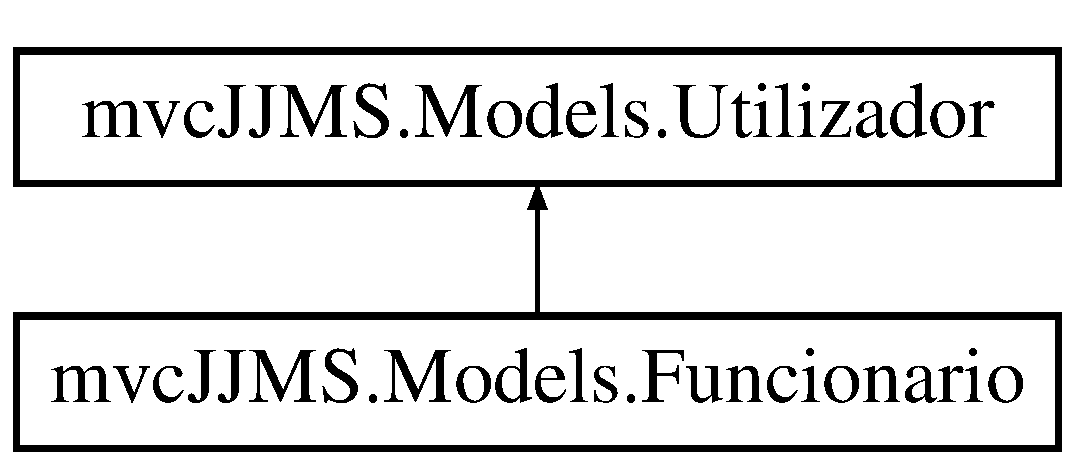
\includegraphics[height=2.000000cm]{classmvc_j_j_m_s_1_1_models_1_1_funcionario}
\end{center}
\end{figure}
\subsection*{Public Member Functions}
\begin{DoxyCompactItemize}
\item 
void \mbox{\hyperlink{classmvc_j_j_m_s_1_1_models_1_1_funcionario_ad694fad2fe71c45f64f40f07a0732f22}{Atualiza\+Avaliacao}} (int classificacao)
\begin{DoxyCompactList}\small\item\em updates the evalution of the employee, calculating the new average \end{DoxyCompactList}\end{DoxyCompactItemize}
\subsection*{Properties}
\begin{DoxyCompactItemize}
\item 
\mbox{\Hypertarget{classmvc_j_j_m_s_1_1_models_1_1_funcionario_a1d25336c62c92efe9a3cd7c94d2cd52b}\label{classmvc_j_j_m_s_1_1_models_1_1_funcionario_a1d25336c62c92efe9a3cd7c94d2cd52b}} 
int {\bfseries Zona\+Trabalho}\hspace{0.3cm}{\ttfamily  \mbox{[}get, set\mbox{]}}
\item 
\mbox{\Hypertarget{classmvc_j_j_m_s_1_1_models_1_1_funcionario_a32517f30e92a5f426e3b3f8d350bf1e5}\label{classmvc_j_j_m_s_1_1_models_1_1_funcionario_a32517f30e92a5f426e3b3f8d350bf1e5}} 
int {\bfseries Nro\+Enc}\hspace{0.3cm}{\ttfamily  \mbox{[}get, set\mbox{]}}
\item 
\mbox{\Hypertarget{classmvc_j_j_m_s_1_1_models_1_1_funcionario_a64c4cd8ca5d1463ba432d7c4129e11db}\label{classmvc_j_j_m_s_1_1_models_1_1_funcionario_a64c4cd8ca5d1463ba432d7c4129e11db}} 
float {\bfseries Avaliação}\hspace{0.3cm}{\ttfamily  \mbox{[}get, set\mbox{]}}
\item 
\mbox{\Hypertarget{classmvc_j_j_m_s_1_1_models_1_1_funcionario_adfcd4c2ca07cafbd73ad933b518e4147}\label{classmvc_j_j_m_s_1_1_models_1_1_funcionario_adfcd4c2ca07cafbd73ad933b518e4147}} 
int {\bfseries Num\+Avaliações}\hspace{0.3cm}{\ttfamily  \mbox{[}get, set\mbox{]}}
\item 
\mbox{\Hypertarget{classmvc_j_j_m_s_1_1_models_1_1_funcionario_a850aa28762c08780a4cbac28d12ed1fa}\label{classmvc_j_j_m_s_1_1_models_1_1_funcionario_a850aa28762c08780a4cbac28d12ed1fa}} 
I\+Collection$<$ \mbox{\hyperlink{classmvc_j_j_m_s_1_1_models_1_1_encomenda}{Encomenda}} $>$ {\bfseries Encomendas}\hspace{0.3cm}{\ttfamily  \mbox{[}get, set\mbox{]}}
\end{DoxyCompactItemize}


\subsection{Detailed Description}
Represents a user of type employee 



\subsection{Member Function Documentation}
\mbox{\Hypertarget{classmvc_j_j_m_s_1_1_models_1_1_funcionario_ad694fad2fe71c45f64f40f07a0732f22}\label{classmvc_j_j_m_s_1_1_models_1_1_funcionario_ad694fad2fe71c45f64f40f07a0732f22}} 
\index{mvc\+J\+J\+M\+S\+::\+Models\+::\+Funcionario@{mvc\+J\+J\+M\+S\+::\+Models\+::\+Funcionario}!Atualiza\+Avaliacao@{Atualiza\+Avaliacao}}
\index{Atualiza\+Avaliacao@{Atualiza\+Avaliacao}!mvc\+J\+J\+M\+S\+::\+Models\+::\+Funcionario@{mvc\+J\+J\+M\+S\+::\+Models\+::\+Funcionario}}
\subsubsection{\texorpdfstring{Atualiza\+Avaliacao()}{AtualizaAvaliacao()}}
{\footnotesize\ttfamily void mvc\+J\+J\+M\+S.\+Models.\+Funcionario.\+Atualiza\+Avaliacao (\begin{DoxyParamCaption}\item[{int}]{classificacao }\end{DoxyParamCaption})\hspace{0.3cm}{\ttfamily [inline]}}



updates the evalution of the employee, calculating the new average 


\begin{DoxyParams}{Parameters}
{\em classificacao} & \\
\hline
\end{DoxyParams}


The documentation for this class was generated from the following file\+:\begin{DoxyCompactItemize}
\item 
Models/Funcionario.\+cs\end{DoxyCompactItemize}

\hypertarget{classmvc_j_j_m_s_1_1_controllers_1_1_funcionario_controller}{}\section{mvc\+J\+J\+M\+S.\+Controllers.\+Funcionario\+Controller Class Reference}
\label{classmvc_j_j_m_s_1_1_controllers_1_1_funcionario_controller}\index{mvc\+J\+J\+M\+S.\+Controllers.\+Funcionario\+Controller@{mvc\+J\+J\+M\+S.\+Controllers.\+Funcionario\+Controller}}
Inheritance diagram for mvc\+J\+J\+M\+S.\+Controllers.\+Funcionario\+Controller\+:\begin{figure}[H]
\begin{center}
\leavevmode
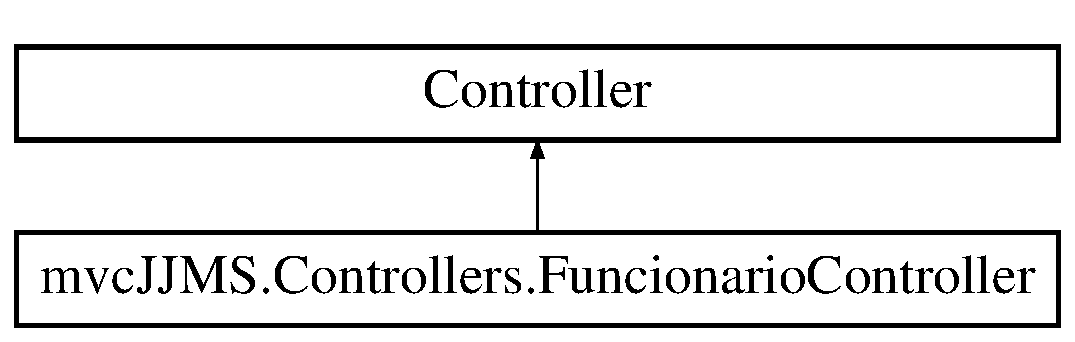
\includegraphics[height=2.000000cm]{classmvc_j_j_m_s_1_1_controllers_1_1_funcionario_controller}
\end{center}
\end{figure}
\subsection*{Public Member Functions}
\begin{DoxyCompactItemize}
\item 
\mbox{\Hypertarget{classmvc_j_j_m_s_1_1_controllers_1_1_funcionario_controller_a757c0fb82ba396715b90fc32f6d9a0a2}\label{classmvc_j_j_m_s_1_1_controllers_1_1_funcionario_controller_a757c0fb82ba396715b90fc32f6d9a0a2}} 
{\bfseries Funcionario\+Controller} (\mbox{\hyperlink{classmvc_j_j_m_s_1_1_data_1_1_j_j_m_s_context}{J\+J\+M\+S\+Context}} context, \mbox{\hyperlink{classmvc_j_j_m_s_1_1_controllers_1_1_utilizador_controller}{Utilizador\+Controller}} u\+Controller, \mbox{\hyperlink{classmvc_j_j_m_s_1_1_controllers_1_1_encomenda_controller}{Encomenda\+Controller}} e\+Controller, \mbox{\hyperlink{classmvc_j_j_m_s_1_1_controllers_1_1_fornecedor_controller}{Fornecedor\+Controller}} f\+Controller)
\item 
\mbox{\hyperlink{classmvc_j_j_m_s_1_1_models_1_1_funcionario}{Funcionario}} \mbox{\hyperlink{classmvc_j_j_m_s_1_1_controllers_1_1_funcionario_controller_a921dda2edb269dfe9a32be22d5abe2ad}{get\+Funcionario}} (int id\+Funcionario)
\begin{DoxyCompactList}\small\item\em return Funcionario(emplyee) with id id\+Funcionario \end{DoxyCompactList}\item 
int \mbox{\hyperlink{classmvc_j_j_m_s_1_1_controllers_1_1_funcionario_controller_a1f66cb42a2fb59a0eaacbcc570cea3ad}{Delegar\+Funcionario}} (int id\+Encomenda, string destino)
\begin{DoxyCompactList}\small\item\em choose an employee to deliver the order with id id\+Encomenda with destino(destiny) adress \end{DoxyCompactList}\item 
void \mbox{\hyperlink{classmvc_j_j_m_s_1_1_controllers_1_1_funcionario_controller_a248cbcd4b3b00e2979d7f6b1ce926505}{Enviar\+Email}} (int id\+Func, int id\+Encomenda)
\begin{DoxyCompactList}\small\item\em sends a email to the choosen employee that will deliver the order with id id\+Encomenda \end{DoxyCompactList}\item 
int \mbox{\hyperlink{classmvc_j_j_m_s_1_1_controllers_1_1_funcionario_controller_a3fc608b887a43ddf67041f09bab3aae5}{Get\+Zona}} (string morada)
\begin{DoxyCompactList}\small\item\em choose the action zone for an employee(\+Not implemented yet) \end{DoxyCompactList}\end{DoxyCompactItemize}


\subsection{Member Function Documentation}
\mbox{\Hypertarget{classmvc_j_j_m_s_1_1_controllers_1_1_funcionario_controller_a1f66cb42a2fb59a0eaacbcc570cea3ad}\label{classmvc_j_j_m_s_1_1_controllers_1_1_funcionario_controller_a1f66cb42a2fb59a0eaacbcc570cea3ad}} 
\index{mvc\+J\+J\+M\+S\+::\+Controllers\+::\+Funcionario\+Controller@{mvc\+J\+J\+M\+S\+::\+Controllers\+::\+Funcionario\+Controller}!Delegar\+Funcionario@{Delegar\+Funcionario}}
\index{Delegar\+Funcionario@{Delegar\+Funcionario}!mvc\+J\+J\+M\+S\+::\+Controllers\+::\+Funcionario\+Controller@{mvc\+J\+J\+M\+S\+::\+Controllers\+::\+Funcionario\+Controller}}
\subsubsection{\texorpdfstring{Delegar\+Funcionario()}{DelegarFuncionario()}}
{\footnotesize\ttfamily int mvc\+J\+J\+M\+S.\+Controllers.\+Funcionario\+Controller.\+Delegar\+Funcionario (\begin{DoxyParamCaption}\item[{int}]{id\+Encomenda,  }\item[{string}]{destino }\end{DoxyParamCaption})\hspace{0.3cm}{\ttfamily [inline]}}



choose an employee to deliver the order with id id\+Encomenda with destino(destiny) adress 


\begin{DoxyParams}{Parameters}
{\em id\+Encomenda} & \\
\hline
{\em destino} & \\
\hline
\end{DoxyParams}
\begin{DoxyReturn}{Returns}
return the id of Funcionario(employee) choosen
\end{DoxyReturn}
\mbox{\Hypertarget{classmvc_j_j_m_s_1_1_controllers_1_1_funcionario_controller_a248cbcd4b3b00e2979d7f6b1ce926505}\label{classmvc_j_j_m_s_1_1_controllers_1_1_funcionario_controller_a248cbcd4b3b00e2979d7f6b1ce926505}} 
\index{mvc\+J\+J\+M\+S\+::\+Controllers\+::\+Funcionario\+Controller@{mvc\+J\+J\+M\+S\+::\+Controllers\+::\+Funcionario\+Controller}!Enviar\+Email@{Enviar\+Email}}
\index{Enviar\+Email@{Enviar\+Email}!mvc\+J\+J\+M\+S\+::\+Controllers\+::\+Funcionario\+Controller@{mvc\+J\+J\+M\+S\+::\+Controllers\+::\+Funcionario\+Controller}}
\subsubsection{\texorpdfstring{Enviar\+Email()}{EnviarEmail()}}
{\footnotesize\ttfamily void mvc\+J\+J\+M\+S.\+Controllers.\+Funcionario\+Controller.\+Enviar\+Email (\begin{DoxyParamCaption}\item[{int}]{id\+Func,  }\item[{int}]{id\+Encomenda }\end{DoxyParamCaption})\hspace{0.3cm}{\ttfamily [inline]}}



sends a email to the choosen employee that will deliver the order with id id\+Encomenda 


\begin{DoxyParams}{Parameters}
{\em id\+Func} & \\
\hline
{\em id\+Encomenda} & \\
\hline
\end{DoxyParams}
\mbox{\Hypertarget{classmvc_j_j_m_s_1_1_controllers_1_1_funcionario_controller_a921dda2edb269dfe9a32be22d5abe2ad}\label{classmvc_j_j_m_s_1_1_controllers_1_1_funcionario_controller_a921dda2edb269dfe9a32be22d5abe2ad}} 
\index{mvc\+J\+J\+M\+S\+::\+Controllers\+::\+Funcionario\+Controller@{mvc\+J\+J\+M\+S\+::\+Controllers\+::\+Funcionario\+Controller}!get\+Funcionario@{get\+Funcionario}}
\index{get\+Funcionario@{get\+Funcionario}!mvc\+J\+J\+M\+S\+::\+Controllers\+::\+Funcionario\+Controller@{mvc\+J\+J\+M\+S\+::\+Controllers\+::\+Funcionario\+Controller}}
\subsubsection{\texorpdfstring{get\+Funcionario()}{getFuncionario()}}
{\footnotesize\ttfamily \mbox{\hyperlink{classmvc_j_j_m_s_1_1_models_1_1_funcionario}{Funcionario}} mvc\+J\+J\+M\+S.\+Controllers.\+Funcionario\+Controller.\+get\+Funcionario (\begin{DoxyParamCaption}\item[{int}]{id\+Funcionario }\end{DoxyParamCaption})\hspace{0.3cm}{\ttfamily [inline]}}



return Funcionario(emplyee) with id id\+Funcionario 


\begin{DoxyParams}{Parameters}
{\em id\+Funcionario} & \\
\hline
\end{DoxyParams}
\begin{DoxyReturn}{Returns}
return Funcionario
\end{DoxyReturn}
\mbox{\Hypertarget{classmvc_j_j_m_s_1_1_controllers_1_1_funcionario_controller_a3fc608b887a43ddf67041f09bab3aae5}\label{classmvc_j_j_m_s_1_1_controllers_1_1_funcionario_controller_a3fc608b887a43ddf67041f09bab3aae5}} 
\index{mvc\+J\+J\+M\+S\+::\+Controllers\+::\+Funcionario\+Controller@{mvc\+J\+J\+M\+S\+::\+Controllers\+::\+Funcionario\+Controller}!Get\+Zona@{Get\+Zona}}
\index{Get\+Zona@{Get\+Zona}!mvc\+J\+J\+M\+S\+::\+Controllers\+::\+Funcionario\+Controller@{mvc\+J\+J\+M\+S\+::\+Controllers\+::\+Funcionario\+Controller}}
\subsubsection{\texorpdfstring{Get\+Zona()}{GetZona()}}
{\footnotesize\ttfamily int mvc\+J\+J\+M\+S.\+Controllers.\+Funcionario\+Controller.\+Get\+Zona (\begin{DoxyParamCaption}\item[{string}]{morada }\end{DoxyParamCaption})\hspace{0.3cm}{\ttfamily [inline]}}



choose the action zone for an employee(\+Not implemented yet) 


\begin{DoxyParams}{Parameters}
{\em morada} & \\
\hline
\end{DoxyParams}
\begin{DoxyReturn}{Returns}
returns the code of the area
\end{DoxyReturn}


The documentation for this class was generated from the following file\+:\begin{DoxyCompactItemize}
\item 
Controllers/Funcionario\+Controller.\+cs\end{DoxyCompactItemize}

\hypertarget{classmvc_j_j_m_s_1_1_data_1_1_j_j_m_s_context}{}\section{mvc\+J\+J\+M\+S.\+Data.\+J\+J\+M\+S\+Context Class Reference}
\label{classmvc_j_j_m_s_1_1_data_1_1_j_j_m_s_context}\index{mvc\+J\+J\+M\+S.\+Data.\+J\+J\+M\+S\+Context@{mvc\+J\+J\+M\+S.\+Data.\+J\+J\+M\+S\+Context}}


Represents a connection to the database with the associated connection string  


Inheritance diagram for mvc\+J\+J\+M\+S.\+Data.\+J\+J\+M\+S\+Context\+:\begin{figure}[H]
\begin{center}
\leavevmode
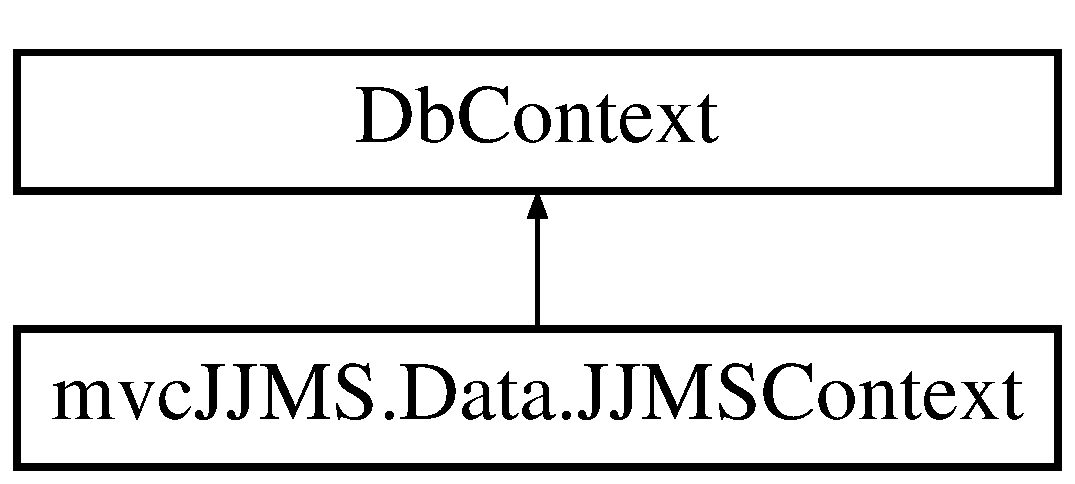
\includegraphics[height=2.000000cm]{classmvc_j_j_m_s_1_1_data_1_1_j_j_m_s_context}
\end{center}
\end{figure}
\subsection*{Public Member Functions}
\begin{DoxyCompactItemize}
\item 
\mbox{\Hypertarget{classmvc_j_j_m_s_1_1_data_1_1_j_j_m_s_context_ab338143e761b1a841c224145bbc0380c}\label{classmvc_j_j_m_s_1_1_data_1_1_j_j_m_s_context_ab338143e761b1a841c224145bbc0380c}} 
{\bfseries J\+J\+M\+S\+Context} (Db\+Context\+Options$<$ \mbox{\hyperlink{classmvc_j_j_m_s_1_1_data_1_1_j_j_m_s_context}{J\+J\+M\+S\+Context}} $>$ options)
\item 
\mbox{\hyperlink{classmvc_j_j_m_s_1_1_models_1_1_fornecedor}{Fornecedor}} \mbox{\hyperlink{classmvc_j_j_m_s_1_1_data_1_1_j_j_m_s_context_aa71841c7b21e94f09c58cbb72c5e7efa}{new\+Fornecedor}} (string nome, string morada)
\begin{DoxyCompactList}\small\item\em Wrapper for creating a new Fornecedor object \end{DoxyCompactList}\item 
\mbox{\hyperlink{classmvc_j_j_m_s_1_1_models_1_1_cliente}{Cliente}} \mbox{\hyperlink{classmvc_j_j_m_s_1_1_data_1_1_j_j_m_s_context_a1daadf80a1157014333476bc1dde9d86}{new\+Cliente}} (string nome, byte\mbox{[}$\,$\mbox{]} passwordH, string email, string morada, string telefone)
\begin{DoxyCompactList}\small\item\em Wrapper for creating a new Cliente object \end{DoxyCompactList}\item 
\mbox{\hyperlink{classmvc_j_j_m_s_1_1_models_1_1_funcionario}{Funcionario}} \mbox{\hyperlink{classmvc_j_j_m_s_1_1_data_1_1_j_j_m_s_context_a2024d653b72abde9d56963ee934605f6}{new\+Funcionario}} (string nome, byte\mbox{[}$\,$\mbox{]} passwordH, string email, int zona\+Trabalho)
\begin{DoxyCompactList}\small\item\em Wrapper for creating a new Funcionario object \end{DoxyCompactList}\item 
\mbox{\hyperlink{classmvc_j_j_m_s_1_1_models_1_1_cartao_credito}{Cartao\+Credito}} \mbox{\hyperlink{classmvc_j_j_m_s_1_1_data_1_1_j_j_m_s_context_ae62a0d5dd75b07b98cc1d6f8e608b256}{new\+Cartao\+Credito}} (long num\+Cartao\+Credito, int mes, int ano, int cvv, string pais)
\begin{DoxyCompactList}\small\item\em Wrapper for creating a new Cartao\+Credito object \end{DoxyCompactList}\item 
\mbox{\hyperlink{classmvc_j_j_m_s_1_1_models_1_1_encomenda}{Encomenda}} \mbox{\hyperlink{classmvc_j_j_m_s_1_1_data_1_1_j_j_m_s_context_ab41e73771fc76a06f3bbbd83df523438}{new\+Encomenda}} (int estado, string destino, Date dia, Time hora, int fornecedor, int cliente, int funcionario, long cc)
\begin{DoxyCompactList}\small\item\em Wrapper for creating a new Encomenda object \end{DoxyCompactList}\end{DoxyCompactItemize}
\subsection*{Protected Member Functions}
\begin{DoxyCompactItemize}
\item 
override void \mbox{\hyperlink{classmvc_j_j_m_s_1_1_data_1_1_j_j_m_s_context_aadc81d0f274fa7d1909d94c7363e5f4a}{On\+Model\+Creating}} (Model\+Builder model\+Builder)
\begin{DoxyCompactList}\small\item\em Registers class attributes as foreign keys and their \end{DoxyCompactList}\end{DoxyCompactItemize}
\subsection*{Properties}
\begin{DoxyCompactItemize}
\item 
Db\+Set$<$ \mbox{\hyperlink{classmvc_j_j_m_s_1_1_models_1_1_cliente}{Cliente}} $>$ \mbox{\hyperlink{classmvc_j_j_m_s_1_1_data_1_1_j_j_m_s_context_af090c3e4b61638096cf0085f313a8bde}{Clientes}}\hspace{0.3cm}{\ttfamily  \mbox{[}get, set\mbox{]}}
\begin{DoxyCompactList}\small\item\em Database table containing client info \end{DoxyCompactList}\item 
Db\+Set$<$ \mbox{\hyperlink{classmvc_j_j_m_s_1_1_models_1_1_funcionario}{Funcionario}} $>$ \mbox{\hyperlink{classmvc_j_j_m_s_1_1_data_1_1_j_j_m_s_context_a8bf23800fa7d55f90d47fb4e227d1fe2}{Funcionarios}}\hspace{0.3cm}{\ttfamily  \mbox{[}get, set\mbox{]}}
\begin{DoxyCompactList}\small\item\em Database table containing employee info \end{DoxyCompactList}\item 
Db\+Set$<$ \mbox{\hyperlink{classmvc_j_j_m_s_1_1_models_1_1_fornecedor}{Fornecedor}} $>$ \mbox{\hyperlink{classmvc_j_j_m_s_1_1_data_1_1_j_j_m_s_context_a46f580334ca10f6fb677d92e21d0778a}{Fornecedores}}\hspace{0.3cm}{\ttfamily  \mbox{[}get, set\mbox{]}}
\begin{DoxyCompactList}\small\item\em Database table containing provider info \end{DoxyCompactList}\item 
Db\+Set$<$ \mbox{\hyperlink{classmvc_j_j_m_s_1_1_models_1_1_encomenda}{Encomenda}} $>$ \mbox{\hyperlink{classmvc_j_j_m_s_1_1_data_1_1_j_j_m_s_context_ad0850c01749a0a69a17ecb59e0d2ed76}{Encomendas}}\hspace{0.3cm}{\ttfamily  \mbox{[}get, set\mbox{]}}
\begin{DoxyCompactList}\small\item\em Database table containing order info \end{DoxyCompactList}\item 
Db\+Set$<$ \mbox{\hyperlink{classmvc_j_j_m_s_1_1_models_1_1_cartao_credito}{Cartao\+Credito}} $>$ \mbox{\hyperlink{classmvc_j_j_m_s_1_1_data_1_1_j_j_m_s_context_aa0df06a1a57e42ddb59661a7f8b38a61}{Cartoes}}\hspace{0.3cm}{\ttfamily  \mbox{[}get, set\mbox{]}}
\begin{DoxyCompactList}\small\item\em Database table containing credit card info \end{DoxyCompactList}\item 
Db\+Set$<$ \mbox{\hyperlink{classmvc_j_j_m_s_1_1_models_1_1_utilizador}{Utilizador}} $>$ \mbox{\hyperlink{classmvc_j_j_m_s_1_1_data_1_1_j_j_m_s_context_a6c5c99292b7657f90a4b24d9da67e4ed}{Utilizadores}}\hspace{0.3cm}{\ttfamily  \mbox{[}get, set\mbox{]}}
\begin{DoxyCompactList}\small\item\em Database table containing user info, both employee and client \end{DoxyCompactList}\end{DoxyCompactItemize}


\subsection{Detailed Description}
Represents a connection to the database with the associated connection string 



\subsection{Member Function Documentation}
\mbox{\Hypertarget{classmvc_j_j_m_s_1_1_data_1_1_j_j_m_s_context_ae62a0d5dd75b07b98cc1d6f8e608b256}\label{classmvc_j_j_m_s_1_1_data_1_1_j_j_m_s_context_ae62a0d5dd75b07b98cc1d6f8e608b256}} 
\index{mvc\+J\+J\+M\+S\+::\+Data\+::\+J\+J\+M\+S\+Context@{mvc\+J\+J\+M\+S\+::\+Data\+::\+J\+J\+M\+S\+Context}!new\+Cartao\+Credito@{new\+Cartao\+Credito}}
\index{new\+Cartao\+Credito@{new\+Cartao\+Credito}!mvc\+J\+J\+M\+S\+::\+Data\+::\+J\+J\+M\+S\+Context@{mvc\+J\+J\+M\+S\+::\+Data\+::\+J\+J\+M\+S\+Context}}
\subsubsection{\texorpdfstring{new\+Cartao\+Credito()}{newCartaoCredito()}}
{\footnotesize\ttfamily \mbox{\hyperlink{classmvc_j_j_m_s_1_1_models_1_1_cartao_credito}{Cartao\+Credito}} mvc\+J\+J\+M\+S.\+Data.\+J\+J\+M\+S\+Context.\+new\+Cartao\+Credito (\begin{DoxyParamCaption}\item[{long}]{num\+Cartao\+Credito,  }\item[{int}]{mes,  }\item[{int}]{ano,  }\item[{int}]{cvv,  }\item[{string}]{pais }\end{DoxyParamCaption})\hspace{0.3cm}{\ttfamily [inline]}}



Wrapper for creating a new Cartao\+Credito object 


\begin{DoxyParams}{Parameters}
{\em num\+Cartao\+Credito} & Credit card number\\
\hline
{\em mes} & Expiration month\\
\hline
{\em ano} & Expiration year\\
\hline
{\em cvv} & Card verification value\\
\hline
{\em pais} & Country of the credit card bank\\
\hline
\end{DoxyParams}
\begin{DoxyReturn}{Returns}
Cartao\+Credito object
\end{DoxyReturn}
\mbox{\Hypertarget{classmvc_j_j_m_s_1_1_data_1_1_j_j_m_s_context_a1daadf80a1157014333476bc1dde9d86}\label{classmvc_j_j_m_s_1_1_data_1_1_j_j_m_s_context_a1daadf80a1157014333476bc1dde9d86}} 
\index{mvc\+J\+J\+M\+S\+::\+Data\+::\+J\+J\+M\+S\+Context@{mvc\+J\+J\+M\+S\+::\+Data\+::\+J\+J\+M\+S\+Context}!new\+Cliente@{new\+Cliente}}
\index{new\+Cliente@{new\+Cliente}!mvc\+J\+J\+M\+S\+::\+Data\+::\+J\+J\+M\+S\+Context@{mvc\+J\+J\+M\+S\+::\+Data\+::\+J\+J\+M\+S\+Context}}
\subsubsection{\texorpdfstring{new\+Cliente()}{newCliente()}}
{\footnotesize\ttfamily \mbox{\hyperlink{classmvc_j_j_m_s_1_1_models_1_1_cliente}{Cliente}} mvc\+J\+J\+M\+S.\+Data.\+J\+J\+M\+S\+Context.\+new\+Cliente (\begin{DoxyParamCaption}\item[{string}]{nome,  }\item[{byte \mbox{[}$\,$\mbox{]}}]{passwordH,  }\item[{string}]{email,  }\item[{string}]{morada,  }\item[{string}]{telefone }\end{DoxyParamCaption})\hspace{0.3cm}{\ttfamily [inline]}}



Wrapper for creating a new Cliente object 


\begin{DoxyParams}{Parameters}
{\em nome} & Username of the client\\
\hline
{\em passwordH} & Client password\\
\hline
{\em email} & Client email\\
\hline
{\em morada} & Client address\\
\hline
{\em telefone} & Client phone number\\
\hline
\end{DoxyParams}
\begin{DoxyReturn}{Returns}
Cliente object
\end{DoxyReturn}
\mbox{\Hypertarget{classmvc_j_j_m_s_1_1_data_1_1_j_j_m_s_context_ab41e73771fc76a06f3bbbd83df523438}\label{classmvc_j_j_m_s_1_1_data_1_1_j_j_m_s_context_ab41e73771fc76a06f3bbbd83df523438}} 
\index{mvc\+J\+J\+M\+S\+::\+Data\+::\+J\+J\+M\+S\+Context@{mvc\+J\+J\+M\+S\+::\+Data\+::\+J\+J\+M\+S\+Context}!new\+Encomenda@{new\+Encomenda}}
\index{new\+Encomenda@{new\+Encomenda}!mvc\+J\+J\+M\+S\+::\+Data\+::\+J\+J\+M\+S\+Context@{mvc\+J\+J\+M\+S\+::\+Data\+::\+J\+J\+M\+S\+Context}}
\subsubsection{\texorpdfstring{new\+Encomenda()}{newEncomenda()}}
{\footnotesize\ttfamily \mbox{\hyperlink{classmvc_j_j_m_s_1_1_models_1_1_encomenda}{Encomenda}} mvc\+J\+J\+M\+S.\+Data.\+J\+J\+M\+S\+Context.\+new\+Encomenda (\begin{DoxyParamCaption}\item[{int}]{estado,  }\item[{string}]{destino,  }\item[{Date}]{dia,  }\item[{Time}]{hora,  }\item[{int}]{fornecedor,  }\item[{int}]{cliente,  }\item[{int}]{funcionario,  }\item[{long}]{cc }\end{DoxyParamCaption})\hspace{0.3cm}{\ttfamily [inline]}}



Wrapper for creating a new Encomenda object 


\begin{DoxyParams}{Parameters}
{\em estado} & Current status on the delivery process\\
\hline
{\em destino} & Destination address\\
\hline
{\em dia} & Delivery day\\
\hline
{\em hora} & Delivery time\\
\hline
{\em fornecedor} & ID of the product provider\\
\hline
{\em cliente} & ID of the client that ordered the product\\
\hline
{\em funcionario} & ID of the employee currently responsible\\
\hline
{\em cc} & Credit card number associated with the order\\
\hline
\end{DoxyParams}
\begin{DoxyReturn}{Returns}
Encomenda object
\end{DoxyReturn}
\mbox{\Hypertarget{classmvc_j_j_m_s_1_1_data_1_1_j_j_m_s_context_aa71841c7b21e94f09c58cbb72c5e7efa}\label{classmvc_j_j_m_s_1_1_data_1_1_j_j_m_s_context_aa71841c7b21e94f09c58cbb72c5e7efa}} 
\index{mvc\+J\+J\+M\+S\+::\+Data\+::\+J\+J\+M\+S\+Context@{mvc\+J\+J\+M\+S\+::\+Data\+::\+J\+J\+M\+S\+Context}!new\+Fornecedor@{new\+Fornecedor}}
\index{new\+Fornecedor@{new\+Fornecedor}!mvc\+J\+J\+M\+S\+::\+Data\+::\+J\+J\+M\+S\+Context@{mvc\+J\+J\+M\+S\+::\+Data\+::\+J\+J\+M\+S\+Context}}
\subsubsection{\texorpdfstring{new\+Fornecedor()}{newFornecedor()}}
{\footnotesize\ttfamily \mbox{\hyperlink{classmvc_j_j_m_s_1_1_models_1_1_fornecedor}{Fornecedor}} mvc\+J\+J\+M\+S.\+Data.\+J\+J\+M\+S\+Context.\+new\+Fornecedor (\begin{DoxyParamCaption}\item[{string}]{nome,  }\item[{string}]{morada }\end{DoxyParamCaption})\hspace{0.3cm}{\ttfamily [inline]}}



Wrapper for creating a new Fornecedor object 


\begin{DoxyParams}{Parameters}
{\em nome} & Name of the provider\\
\hline
{\em morada} & Address of the provider\\
\hline
\end{DoxyParams}
\begin{DoxyReturn}{Returns}
Fornecedor object
\end{DoxyReturn}
\mbox{\Hypertarget{classmvc_j_j_m_s_1_1_data_1_1_j_j_m_s_context_a2024d653b72abde9d56963ee934605f6}\label{classmvc_j_j_m_s_1_1_data_1_1_j_j_m_s_context_a2024d653b72abde9d56963ee934605f6}} 
\index{mvc\+J\+J\+M\+S\+::\+Data\+::\+J\+J\+M\+S\+Context@{mvc\+J\+J\+M\+S\+::\+Data\+::\+J\+J\+M\+S\+Context}!new\+Funcionario@{new\+Funcionario}}
\index{new\+Funcionario@{new\+Funcionario}!mvc\+J\+J\+M\+S\+::\+Data\+::\+J\+J\+M\+S\+Context@{mvc\+J\+J\+M\+S\+::\+Data\+::\+J\+J\+M\+S\+Context}}
\subsubsection{\texorpdfstring{new\+Funcionario()}{newFuncionario()}}
{\footnotesize\ttfamily \mbox{\hyperlink{classmvc_j_j_m_s_1_1_models_1_1_funcionario}{Funcionario}} mvc\+J\+J\+M\+S.\+Data.\+J\+J\+M\+S\+Context.\+new\+Funcionario (\begin{DoxyParamCaption}\item[{string}]{nome,  }\item[{byte \mbox{[}$\,$\mbox{]}}]{passwordH,  }\item[{string}]{email,  }\item[{int}]{zona\+Trabalho }\end{DoxyParamCaption})\hspace{0.3cm}{\ttfamily [inline]}}



Wrapper for creating a new Funcionario object 


\begin{DoxyParams}{Parameters}
{\em nome} & Username of the employee\\
\hline
{\em passwordH} & Employee password\\
\hline
{\em email} & Employee email\\
\hline
{\em zona\+Trabalho} & Identifier of the work zone that the employee is assigned\\
\hline
\end{DoxyParams}
\begin{DoxyReturn}{Returns}
Funcionario object
\end{DoxyReturn}
\mbox{\Hypertarget{classmvc_j_j_m_s_1_1_data_1_1_j_j_m_s_context_aadc81d0f274fa7d1909d94c7363e5f4a}\label{classmvc_j_j_m_s_1_1_data_1_1_j_j_m_s_context_aadc81d0f274fa7d1909d94c7363e5f4a}} 
\index{mvc\+J\+J\+M\+S\+::\+Data\+::\+J\+J\+M\+S\+Context@{mvc\+J\+J\+M\+S\+::\+Data\+::\+J\+J\+M\+S\+Context}!On\+Model\+Creating@{On\+Model\+Creating}}
\index{On\+Model\+Creating@{On\+Model\+Creating}!mvc\+J\+J\+M\+S\+::\+Data\+::\+J\+J\+M\+S\+Context@{mvc\+J\+J\+M\+S\+::\+Data\+::\+J\+J\+M\+S\+Context}}
\subsubsection{\texorpdfstring{On\+Model\+Creating()}{OnModelCreating()}}
{\footnotesize\ttfamily override void mvc\+J\+J\+M\+S.\+Data.\+J\+J\+M\+S\+Context.\+On\+Model\+Creating (\begin{DoxyParamCaption}\item[{Model\+Builder}]{model\+Builder }\end{DoxyParamCaption})\hspace{0.3cm}{\ttfamily [inline]}, {\ttfamily [protected]}}



Registers class attributes as foreign keys and their 


\begin{DoxyParams}{Parameters}
{\em model\+Builder} & \\
\hline
\end{DoxyParams}


\subsection{Property Documentation}
\mbox{\Hypertarget{classmvc_j_j_m_s_1_1_data_1_1_j_j_m_s_context_aa0df06a1a57e42ddb59661a7f8b38a61}\label{classmvc_j_j_m_s_1_1_data_1_1_j_j_m_s_context_aa0df06a1a57e42ddb59661a7f8b38a61}} 
\index{mvc\+J\+J\+M\+S\+::\+Data\+::\+J\+J\+M\+S\+Context@{mvc\+J\+J\+M\+S\+::\+Data\+::\+J\+J\+M\+S\+Context}!Cartoes@{Cartoes}}
\index{Cartoes@{Cartoes}!mvc\+J\+J\+M\+S\+::\+Data\+::\+J\+J\+M\+S\+Context@{mvc\+J\+J\+M\+S\+::\+Data\+::\+J\+J\+M\+S\+Context}}
\subsubsection{\texorpdfstring{Cartoes}{Cartoes}}
{\footnotesize\ttfamily Db\+Set$<$\mbox{\hyperlink{classmvc_j_j_m_s_1_1_models_1_1_cartao_credito}{Cartao\+Credito}}$>$ mvc\+J\+J\+M\+S.\+Data.\+J\+J\+M\+S\+Context.\+Cartoes\hspace{0.3cm}{\ttfamily [get]}, {\ttfamily [set]}}



Database table containing credit card info 

\mbox{\Hypertarget{classmvc_j_j_m_s_1_1_data_1_1_j_j_m_s_context_af090c3e4b61638096cf0085f313a8bde}\label{classmvc_j_j_m_s_1_1_data_1_1_j_j_m_s_context_af090c3e4b61638096cf0085f313a8bde}} 
\index{mvc\+J\+J\+M\+S\+::\+Data\+::\+J\+J\+M\+S\+Context@{mvc\+J\+J\+M\+S\+::\+Data\+::\+J\+J\+M\+S\+Context}!Clientes@{Clientes}}
\index{Clientes@{Clientes}!mvc\+J\+J\+M\+S\+::\+Data\+::\+J\+J\+M\+S\+Context@{mvc\+J\+J\+M\+S\+::\+Data\+::\+J\+J\+M\+S\+Context}}
\subsubsection{\texorpdfstring{Clientes}{Clientes}}
{\footnotesize\ttfamily Db\+Set$<$\mbox{\hyperlink{classmvc_j_j_m_s_1_1_models_1_1_cliente}{Cliente}}$>$ mvc\+J\+J\+M\+S.\+Data.\+J\+J\+M\+S\+Context.\+Clientes\hspace{0.3cm}{\ttfamily [get]}, {\ttfamily [set]}}



Database table containing client info 

\mbox{\Hypertarget{classmvc_j_j_m_s_1_1_data_1_1_j_j_m_s_context_ad0850c01749a0a69a17ecb59e0d2ed76}\label{classmvc_j_j_m_s_1_1_data_1_1_j_j_m_s_context_ad0850c01749a0a69a17ecb59e0d2ed76}} 
\index{mvc\+J\+J\+M\+S\+::\+Data\+::\+J\+J\+M\+S\+Context@{mvc\+J\+J\+M\+S\+::\+Data\+::\+J\+J\+M\+S\+Context}!Encomendas@{Encomendas}}
\index{Encomendas@{Encomendas}!mvc\+J\+J\+M\+S\+::\+Data\+::\+J\+J\+M\+S\+Context@{mvc\+J\+J\+M\+S\+::\+Data\+::\+J\+J\+M\+S\+Context}}
\subsubsection{\texorpdfstring{Encomendas}{Encomendas}}
{\footnotesize\ttfamily Db\+Set$<$\mbox{\hyperlink{classmvc_j_j_m_s_1_1_models_1_1_encomenda}{Encomenda}}$>$ mvc\+J\+J\+M\+S.\+Data.\+J\+J\+M\+S\+Context.\+Encomendas\hspace{0.3cm}{\ttfamily [get]}, {\ttfamily [set]}}



Database table containing order info 

\mbox{\Hypertarget{classmvc_j_j_m_s_1_1_data_1_1_j_j_m_s_context_a46f580334ca10f6fb677d92e21d0778a}\label{classmvc_j_j_m_s_1_1_data_1_1_j_j_m_s_context_a46f580334ca10f6fb677d92e21d0778a}} 
\index{mvc\+J\+J\+M\+S\+::\+Data\+::\+J\+J\+M\+S\+Context@{mvc\+J\+J\+M\+S\+::\+Data\+::\+J\+J\+M\+S\+Context}!Fornecedores@{Fornecedores}}
\index{Fornecedores@{Fornecedores}!mvc\+J\+J\+M\+S\+::\+Data\+::\+J\+J\+M\+S\+Context@{mvc\+J\+J\+M\+S\+::\+Data\+::\+J\+J\+M\+S\+Context}}
\subsubsection{\texorpdfstring{Fornecedores}{Fornecedores}}
{\footnotesize\ttfamily Db\+Set$<$\mbox{\hyperlink{classmvc_j_j_m_s_1_1_models_1_1_fornecedor}{Fornecedor}}$>$ mvc\+J\+J\+M\+S.\+Data.\+J\+J\+M\+S\+Context.\+Fornecedores\hspace{0.3cm}{\ttfamily [get]}, {\ttfamily [set]}}



Database table containing provider info 

\mbox{\Hypertarget{classmvc_j_j_m_s_1_1_data_1_1_j_j_m_s_context_a8bf23800fa7d55f90d47fb4e227d1fe2}\label{classmvc_j_j_m_s_1_1_data_1_1_j_j_m_s_context_a8bf23800fa7d55f90d47fb4e227d1fe2}} 
\index{mvc\+J\+J\+M\+S\+::\+Data\+::\+J\+J\+M\+S\+Context@{mvc\+J\+J\+M\+S\+::\+Data\+::\+J\+J\+M\+S\+Context}!Funcionarios@{Funcionarios}}
\index{Funcionarios@{Funcionarios}!mvc\+J\+J\+M\+S\+::\+Data\+::\+J\+J\+M\+S\+Context@{mvc\+J\+J\+M\+S\+::\+Data\+::\+J\+J\+M\+S\+Context}}
\subsubsection{\texorpdfstring{Funcionarios}{Funcionarios}}
{\footnotesize\ttfamily Db\+Set$<$\mbox{\hyperlink{classmvc_j_j_m_s_1_1_models_1_1_funcionario}{Funcionario}}$>$ mvc\+J\+J\+M\+S.\+Data.\+J\+J\+M\+S\+Context.\+Funcionarios\hspace{0.3cm}{\ttfamily [get]}, {\ttfamily [set]}}



Database table containing employee info 

\mbox{\Hypertarget{classmvc_j_j_m_s_1_1_data_1_1_j_j_m_s_context_a6c5c99292b7657f90a4b24d9da67e4ed}\label{classmvc_j_j_m_s_1_1_data_1_1_j_j_m_s_context_a6c5c99292b7657f90a4b24d9da67e4ed}} 
\index{mvc\+J\+J\+M\+S\+::\+Data\+::\+J\+J\+M\+S\+Context@{mvc\+J\+J\+M\+S\+::\+Data\+::\+J\+J\+M\+S\+Context}!Utilizadores@{Utilizadores}}
\index{Utilizadores@{Utilizadores}!mvc\+J\+J\+M\+S\+::\+Data\+::\+J\+J\+M\+S\+Context@{mvc\+J\+J\+M\+S\+::\+Data\+::\+J\+J\+M\+S\+Context}}
\subsubsection{\texorpdfstring{Utilizadores}{Utilizadores}}
{\footnotesize\ttfamily Db\+Set$<$\mbox{\hyperlink{classmvc_j_j_m_s_1_1_models_1_1_utilizador}{Utilizador}}$>$ mvc\+J\+J\+M\+S.\+Data.\+J\+J\+M\+S\+Context.\+Utilizadores\hspace{0.3cm}{\ttfamily [get]}, {\ttfamily [set]}}



Database table containing user info, both employee and client 



The documentation for this class was generated from the following file\+:\begin{DoxyCompactItemize}
\item 
Data/J\+J\+M\+S\+Context.\+cs\end{DoxyCompactItemize}

\hypertarget{classmvc_j_j_m_s_1_1_controllers_1_1_menu_cliente_controller}{}\section{mvc\+J\+J\+M\+S.\+Controllers.\+Menu\+Cliente\+Controller Class Reference}
\label{classmvc_j_j_m_s_1_1_controllers_1_1_menu_cliente_controller}\index{mvc\+J\+J\+M\+S.\+Controllers.\+Menu\+Cliente\+Controller@{mvc\+J\+J\+M\+S.\+Controllers.\+Menu\+Cliente\+Controller}}
Inheritance diagram for mvc\+J\+J\+M\+S.\+Controllers.\+Menu\+Cliente\+Controller\+:\begin{figure}[H]
\begin{center}
\leavevmode
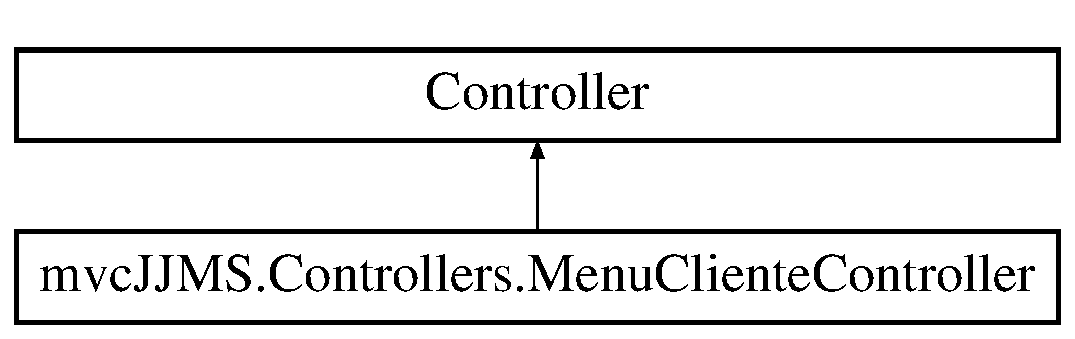
\includegraphics[height=2.000000cm]{classmvc_j_j_m_s_1_1_controllers_1_1_menu_cliente_controller}
\end{center}
\end{figure}
\subsection*{Public Member Functions}
\begin{DoxyCompactItemize}
\item 
\mbox{\Hypertarget{classmvc_j_j_m_s_1_1_controllers_1_1_menu_cliente_controller_a255074854d91d443c60f47991a493d03}\label{classmvc_j_j_m_s_1_1_controllers_1_1_menu_cliente_controller_a255074854d91d443c60f47991a493d03}} 
{\bfseries Menu\+Cliente\+Controller} (\mbox{\hyperlink{classmvc_j_j_m_s_1_1_data_1_1_j_j_m_s_context}{J\+J\+M\+S\+Context}} context, \mbox{\hyperlink{classmvc_j_j_m_s_1_1_controllers_1_1_encomenda_controller}{Encomenda\+Controller}} e\+Controller, \mbox{\hyperlink{classmvc_j_j_m_s_1_1_controllers_1_1_utilizador_controller}{Utilizador\+Controller}} u\+Controller, \mbox{\hyperlink{classmvc_j_j_m_s_1_1_controllers_1_1_cliente_controller}{Cliente\+Controller}} c\+Controller, \mbox{\hyperlink{classmvc_j_j_m_s_1_1_controllers_1_1_funcionario_controller}{Funcionario\+Controller}} f\+Controller)
\item 
\mbox{\Hypertarget{classmvc_j_j_m_s_1_1_controllers_1_1_menu_cliente_controller_a60f79627774e8151c0d87dd1971ca3ae}\label{classmvc_j_j_m_s_1_1_controllers_1_1_menu_cliente_controller_a60f79627774e8151c0d87dd1971ca3ae}} 
View\+Result {\bfseries Index} ()
\item 
View\+Result \mbox{\hyperlink{classmvc_j_j_m_s_1_1_controllers_1_1_menu_cliente_controller_abfae9a2d4e35be83a5baf81cb906d41e}{Tracking\+Encomenda}} ()
\begin{DoxyCompactList}\small\item\em Wrapper for the Tracking\+Encomenda method on the \mbox{\hyperlink{classmvc_j_j_m_s_1_1_controllers_1_1_encomenda_controller}{Encomenda\+Controller}} \end{DoxyCompactList}\item 
\mbox{\Hypertarget{classmvc_j_j_m_s_1_1_controllers_1_1_menu_cliente_controller_aac2a018e346fbc50fc186d672e04ac32}\label{classmvc_j_j_m_s_1_1_controllers_1_1_menu_cliente_controller_aac2a018e346fbc50fc186d672e04ac32}} 
View\+Result {\bfseries Cancelar\+Tracking} ()
\item 
\mbox{\Hypertarget{classmvc_j_j_m_s_1_1_controllers_1_1_menu_cliente_controller_a939a097483e0d3ccfab5dc33809630c6}\label{classmvc_j_j_m_s_1_1_controllers_1_1_menu_cliente_controller_a939a097483e0d3ccfab5dc33809630c6}} 
View\+Result {\bfseries Avaliar\+Servico} ()
\item 
\mbox{\Hypertarget{classmvc_j_j_m_s_1_1_controllers_1_1_menu_cliente_controller_af438b7423cb0804aa219325081c070aa}\label{classmvc_j_j_m_s_1_1_controllers_1_1_menu_cliente_controller_af438b7423cb0804aa219325081c070aa}} 
View\+Result {\bfseries Alterar\+Dados} ()
\item 
Action\+Result \mbox{\hyperlink{classmvc_j_j_m_s_1_1_controllers_1_1_menu_cliente_controller_a2d3e5123426f07356591f476a5c2e6e1}{Alterar\+Dados\+Alterar}} (string nome\+Input, string password\+Input, string email\+Input, string morada\+Input, string telefone\+Input)
\begin{DoxyCompactList}\small\item\em Changes the user data associated with the user currently logged in \end{DoxyCompactList}\item 
\mbox{\Hypertarget{classmvc_j_j_m_s_1_1_controllers_1_1_menu_cliente_controller_a50b8d888b8de031e1f43c07c054bdf58}\label{classmvc_j_j_m_s_1_1_controllers_1_1_menu_cliente_controller_a50b8d888b8de031e1f43c07c054bdf58}} 
View\+Result {\bfseries Alterado\+Com\+Sucesso} ()
\item 
\mbox{\Hypertarget{classmvc_j_j_m_s_1_1_controllers_1_1_menu_cliente_controller_a586996d6bf82b8d0faa217148eaceaca}\label{classmvc_j_j_m_s_1_1_controllers_1_1_menu_cliente_controller_a586996d6bf82b8d0faa217148eaceaca}} 
View\+Result {\bfseries Email\+Ja\+Associado} ()
\item 
\mbox{\Hypertarget{classmvc_j_j_m_s_1_1_controllers_1_1_menu_cliente_controller_a01b37f1fc945e60b337ec9288548c404}\label{classmvc_j_j_m_s_1_1_controllers_1_1_menu_cliente_controller_a01b37f1fc945e60b337ec9288548c404}} 
View\+Result {\bfseries Telefone\+Invalido} ()
\item 
\mbox{\Hypertarget{classmvc_j_j_m_s_1_1_controllers_1_1_menu_cliente_controller_af542ed6304021c156ad94acd5fed451b}\label{classmvc_j_j_m_s_1_1_controllers_1_1_menu_cliente_controller_af542ed6304021c156ad94acd5fed451b}} 
View\+Result {\bfseries Password\+Insegura} ()
\item 
\mbox{\Hypertarget{classmvc_j_j_m_s_1_1_controllers_1_1_menu_cliente_controller_ab98994021cafc5f2d7138660fbddb56e}\label{classmvc_j_j_m_s_1_1_controllers_1_1_menu_cliente_controller_ab98994021cafc5f2d7138660fbddb56e}} 
View\+Result {\bfseries Cancelar\+Avaliar} ()
\item 
Action\+Result \mbox{\hyperlink{classmvc_j_j_m_s_1_1_controllers_1_1_menu_cliente_controller_a80c955969df7336ef727d73da76caa66}{check\+Encomenda}} (int id\+Encomenda)
\begin{DoxyCompactList}\small\item\em Checks whether the order is eligible to be rated \end{DoxyCompactList}\item 
\mbox{\Hypertarget{classmvc_j_j_m_s_1_1_controllers_1_1_menu_cliente_controller_a9104ae784f8a690120c3fd46c2f28909}\label{classmvc_j_j_m_s_1_1_controllers_1_1_menu_cliente_controller_a9104ae784f8a690120c3fd46c2f28909}} 
View\+Result {\bfseries Codigo\+Inexistente} ()
\item 
\mbox{\Hypertarget{classmvc_j_j_m_s_1_1_controllers_1_1_menu_cliente_controller_aaa920273d6cb8cd5dd28785c21c2d795}\label{classmvc_j_j_m_s_1_1_controllers_1_1_menu_cliente_controller_aaa920273d6cb8cd5dd28785c21c2d795}} 
View\+Result {\bfseries Encomenda\+Por\+Entregar} ()
\item 
\mbox{\Hypertarget{classmvc_j_j_m_s_1_1_controllers_1_1_menu_cliente_controller_a0ccc43b32da53fb0cd59665b7023f266}\label{classmvc_j_j_m_s_1_1_controllers_1_1_menu_cliente_controller_a0ccc43b32da53fb0cd59665b7023f266}} 
View\+Result {\bfseries Inserir\+Classificacoes} (int id\+Encomenda)
\item 
Action\+Result \mbox{\hyperlink{classmvc_j_j_m_s_1_1_controllers_1_1_menu_cliente_controller_a1e42ec4e15eda326d61aed409dab3a97}{AvaliaS}} (string id\+EncomendaS, int class\+Servico\+Entrega, int class\+Estado\+Encomenda)
\begin{DoxyCompactList}\small\item\em Wrapper to the avalia method \end{DoxyCompactList}\item 
bool \mbox{\hyperlink{classmvc_j_j_m_s_1_1_controllers_1_1_menu_cliente_controller_af0c08fdfd46b358fce2002e705daba6b}{classificacoes\+Validas}} (int class\+Servico\+Entrega, int class\+Estado\+Encomenda)
\begin{DoxyCompactList}\small\item\em Checks whether the ratings are within the predefined ranges \end{DoxyCompactList}\item 
void \mbox{\hyperlink{classmvc_j_j_m_s_1_1_controllers_1_1_menu_cliente_controller_a115e3395ec215fd48a75dc140232b7fe}{avalia}} (int id\+Encomenda, int class\+Servico\+Entrega, int class\+Estado\+Encomenda)
\begin{DoxyCompactList}\small\item\em Registers a service rating referring to a given order \end{DoxyCompactList}\item 
\mbox{\Hypertarget{classmvc_j_j_m_s_1_1_controllers_1_1_menu_cliente_controller_a328510da7f857e253e57ac44de6de83c}\label{classmvc_j_j_m_s_1_1_controllers_1_1_menu_cliente_controller_a328510da7f857e253e57ac44de6de83c}} 
View\+Result {\bfseries Classificaoes\+Invalidas} ()
\item 
\mbox{\Hypertarget{classmvc_j_j_m_s_1_1_controllers_1_1_menu_cliente_controller_afc3a11add77380e9cef2ca9a48ff6169}\label{classmvc_j_j_m_s_1_1_controllers_1_1_menu_cliente_controller_afc3a11add77380e9cef2ca9a48ff6169}} 
View\+Result {\bfseries Sucesso} ()
\item 
async Task$<$ I\+Action\+Result $>$ \mbox{\hyperlink{classmvc_j_j_m_s_1_1_controllers_1_1_menu_cliente_controller_a6aadfeccdbb52ae6a555b2ee00c4a3f0}{Consultar\+Historico}} ()
\begin{DoxyCompactList}\small\item\em Redirects to a screen containing all the orders associated with the currently logged in user \end{DoxyCompactList}\item 
\mbox{\Hypertarget{classmvc_j_j_m_s_1_1_controllers_1_1_menu_cliente_controller_a91fd91fa2b700ee34740d2e68fb0d40f}\label{classmvc_j_j_m_s_1_1_controllers_1_1_menu_cliente_controller_a91fd91fa2b700ee34740d2e68fb0d40f}} 
View\+Result {\bfseries Requisitar\+Encomenda} ()
\item 
\mbox{\Hypertarget{classmvc_j_j_m_s_1_1_controllers_1_1_menu_cliente_controller_a4aa4e2445d00a056a9d5727676e65704}\label{classmvc_j_j_m_s_1_1_controllers_1_1_menu_cliente_controller_a4aa4e2445d00a056a9d5727676e65704}} 
View\+Result {\bfseries Cliente\+Bloqueado} ()
\end{DoxyCompactItemize}


\subsection{Member Function Documentation}
\mbox{\Hypertarget{classmvc_j_j_m_s_1_1_controllers_1_1_menu_cliente_controller_a2d3e5123426f07356591f476a5c2e6e1}\label{classmvc_j_j_m_s_1_1_controllers_1_1_menu_cliente_controller_a2d3e5123426f07356591f476a5c2e6e1}} 
\index{mvc\+J\+J\+M\+S\+::\+Controllers\+::\+Menu\+Cliente\+Controller@{mvc\+J\+J\+M\+S\+::\+Controllers\+::\+Menu\+Cliente\+Controller}!Alterar\+Dados\+Alterar@{Alterar\+Dados\+Alterar}}
\index{Alterar\+Dados\+Alterar@{Alterar\+Dados\+Alterar}!mvc\+J\+J\+M\+S\+::\+Controllers\+::\+Menu\+Cliente\+Controller@{mvc\+J\+J\+M\+S\+::\+Controllers\+::\+Menu\+Cliente\+Controller}}
\subsubsection{\texorpdfstring{Alterar\+Dados\+Alterar()}{AlterarDadosAlterar()}}
{\footnotesize\ttfamily Action\+Result mvc\+J\+J\+M\+S.\+Controllers.\+Menu\+Cliente\+Controller.\+Alterar\+Dados\+Alterar (\begin{DoxyParamCaption}\item[{string}]{nome\+Input,  }\item[{string}]{password\+Input,  }\item[{string}]{email\+Input,  }\item[{string}]{morada\+Input,  }\item[{string}]{telefone\+Input }\end{DoxyParamCaption})\hspace{0.3cm}{\ttfamily [inline]}}



Changes the user data associated with the user currently logged in 


\begin{DoxyParams}{Parameters}
{\em nome\+Input} & New value for Nome\\
\hline
{\em password\+Input} & New password\\
\hline
{\em email\+Input} & New user email\\
\hline
{\em morada\+Input} & New user address\\
\hline
{\em telefone\+Input} & New user phone number\\
\hline
\end{DoxyParams}
\begin{DoxyReturn}{Returns}
Redirects to a Sucess screen of an Error view
\end{DoxyReturn}
\mbox{\Hypertarget{classmvc_j_j_m_s_1_1_controllers_1_1_menu_cliente_controller_a115e3395ec215fd48a75dc140232b7fe}\label{classmvc_j_j_m_s_1_1_controllers_1_1_menu_cliente_controller_a115e3395ec215fd48a75dc140232b7fe}} 
\index{mvc\+J\+J\+M\+S\+::\+Controllers\+::\+Menu\+Cliente\+Controller@{mvc\+J\+J\+M\+S\+::\+Controllers\+::\+Menu\+Cliente\+Controller}!avalia@{avalia}}
\index{avalia@{avalia}!mvc\+J\+J\+M\+S\+::\+Controllers\+::\+Menu\+Cliente\+Controller@{mvc\+J\+J\+M\+S\+::\+Controllers\+::\+Menu\+Cliente\+Controller}}
\subsubsection{\texorpdfstring{avalia()}{avalia()}}
{\footnotesize\ttfamily void mvc\+J\+J\+M\+S.\+Controllers.\+Menu\+Cliente\+Controller.\+avalia (\begin{DoxyParamCaption}\item[{int}]{id\+Encomenda,  }\item[{int}]{class\+Servico\+Entrega,  }\item[{int}]{class\+Estado\+Encomenda }\end{DoxyParamCaption})\hspace{0.3cm}{\ttfamily [inline]}}



Registers a service rating referring to a given order 


\begin{DoxyParams}{Parameters}
{\em id\+Encomenda} & Unique identifier for a single order\\
\hline
{\em class\+Servico\+Entrega} & Rating relating to the employee\\
\hline
{\em class\+Estado\+Encomenda} & Rating relating to the order\\
\hline
\end{DoxyParams}
\mbox{\Hypertarget{classmvc_j_j_m_s_1_1_controllers_1_1_menu_cliente_controller_a1e42ec4e15eda326d61aed409dab3a97}\label{classmvc_j_j_m_s_1_1_controllers_1_1_menu_cliente_controller_a1e42ec4e15eda326d61aed409dab3a97}} 
\index{mvc\+J\+J\+M\+S\+::\+Controllers\+::\+Menu\+Cliente\+Controller@{mvc\+J\+J\+M\+S\+::\+Controllers\+::\+Menu\+Cliente\+Controller}!AvaliaS@{AvaliaS}}
\index{AvaliaS@{AvaliaS}!mvc\+J\+J\+M\+S\+::\+Controllers\+::\+Menu\+Cliente\+Controller@{mvc\+J\+J\+M\+S\+::\+Controllers\+::\+Menu\+Cliente\+Controller}}
\subsubsection{\texorpdfstring{Avalia\+S()}{AvaliaS()}}
{\footnotesize\ttfamily Action\+Result mvc\+J\+J\+M\+S.\+Controllers.\+Menu\+Cliente\+Controller.\+AvaliaS (\begin{DoxyParamCaption}\item[{string}]{id\+EncomendaS,  }\item[{int}]{class\+Servico\+Entrega,  }\item[{int}]{class\+Estado\+Encomenda }\end{DoxyParamCaption})\hspace{0.3cm}{\ttfamily [inline]}}



Wrapper to the avalia method 


\begin{DoxyParams}{Parameters}
{\em id\+EncomendaS} & Unique identifier for a single order in a string format\\
\hline
{\em class\+Servico\+Entrega} & Rating relating to the employee\\
\hline
{\em class\+Estado\+Encomenda} & Rating relating to the order\\
\hline
\end{DoxyParams}
\begin{DoxyReturn}{Returns}
Redirects to the Sucess view or to an Error view if invalid ratings are given
\end{DoxyReturn}
\mbox{\Hypertarget{classmvc_j_j_m_s_1_1_controllers_1_1_menu_cliente_controller_a80c955969df7336ef727d73da76caa66}\label{classmvc_j_j_m_s_1_1_controllers_1_1_menu_cliente_controller_a80c955969df7336ef727d73da76caa66}} 
\index{mvc\+J\+J\+M\+S\+::\+Controllers\+::\+Menu\+Cliente\+Controller@{mvc\+J\+J\+M\+S\+::\+Controllers\+::\+Menu\+Cliente\+Controller}!check\+Encomenda@{check\+Encomenda}}
\index{check\+Encomenda@{check\+Encomenda}!mvc\+J\+J\+M\+S\+::\+Controllers\+::\+Menu\+Cliente\+Controller@{mvc\+J\+J\+M\+S\+::\+Controllers\+::\+Menu\+Cliente\+Controller}}
\subsubsection{\texorpdfstring{check\+Encomenda()}{checkEncomenda()}}
{\footnotesize\ttfamily Action\+Result mvc\+J\+J\+M\+S.\+Controllers.\+Menu\+Cliente\+Controller.\+check\+Encomenda (\begin{DoxyParamCaption}\item[{int}]{id\+Encomenda }\end{DoxyParamCaption})\hspace{0.3cm}{\ttfamily [inline]}}



Checks whether the order is eligible to be rated 


\begin{DoxyParams}{Parameters}
{\em id\+Encomenda} & Unique identifier for a single order\\
\hline
\end{DoxyParams}
\begin{DoxyReturn}{Returns}
Redirects to the Rating Menu or to an Error view
\end{DoxyReturn}
\mbox{\Hypertarget{classmvc_j_j_m_s_1_1_controllers_1_1_menu_cliente_controller_af0c08fdfd46b358fce2002e705daba6b}\label{classmvc_j_j_m_s_1_1_controllers_1_1_menu_cliente_controller_af0c08fdfd46b358fce2002e705daba6b}} 
\index{mvc\+J\+J\+M\+S\+::\+Controllers\+::\+Menu\+Cliente\+Controller@{mvc\+J\+J\+M\+S\+::\+Controllers\+::\+Menu\+Cliente\+Controller}!classificacoes\+Validas@{classificacoes\+Validas}}
\index{classificacoes\+Validas@{classificacoes\+Validas}!mvc\+J\+J\+M\+S\+::\+Controllers\+::\+Menu\+Cliente\+Controller@{mvc\+J\+J\+M\+S\+::\+Controllers\+::\+Menu\+Cliente\+Controller}}
\subsubsection{\texorpdfstring{classificacoes\+Validas()}{classificacoesValidas()}}
{\footnotesize\ttfamily bool mvc\+J\+J\+M\+S.\+Controllers.\+Menu\+Cliente\+Controller.\+classificacoes\+Validas (\begin{DoxyParamCaption}\item[{int}]{class\+Servico\+Entrega,  }\item[{int}]{class\+Estado\+Encomenda }\end{DoxyParamCaption})\hspace{0.3cm}{\ttfamily [inline]}}



Checks whether the ratings are within the predefined ranges 


\begin{DoxyParams}{Parameters}
{\em class\+Servico\+Entrega} & Rating relating to the employee\\
\hline
{\em class\+Estado\+Encomenda} & Rating relating to the order\\
\hline
\end{DoxyParams}
\begin{DoxyReturn}{Returns}
T\+R\+UE if the ratings are valid else F\+A\+L\+SE
\end{DoxyReturn}
\mbox{\Hypertarget{classmvc_j_j_m_s_1_1_controllers_1_1_menu_cliente_controller_a6aadfeccdbb52ae6a555b2ee00c4a3f0}\label{classmvc_j_j_m_s_1_1_controllers_1_1_menu_cliente_controller_a6aadfeccdbb52ae6a555b2ee00c4a3f0}} 
\index{mvc\+J\+J\+M\+S\+::\+Controllers\+::\+Menu\+Cliente\+Controller@{mvc\+J\+J\+M\+S\+::\+Controllers\+::\+Menu\+Cliente\+Controller}!Consultar\+Historico@{Consultar\+Historico}}
\index{Consultar\+Historico@{Consultar\+Historico}!mvc\+J\+J\+M\+S\+::\+Controllers\+::\+Menu\+Cliente\+Controller@{mvc\+J\+J\+M\+S\+::\+Controllers\+::\+Menu\+Cliente\+Controller}}
\subsubsection{\texorpdfstring{Consultar\+Historico()}{ConsultarHistorico()}}
{\footnotesize\ttfamily async Task$<$I\+Action\+Result$>$ mvc\+J\+J\+M\+S.\+Controllers.\+Menu\+Cliente\+Controller.\+Consultar\+Historico (\begin{DoxyParamCaption}{ }\end{DoxyParamCaption})\hspace{0.3cm}{\ttfamily [inline]}}



Redirects to a screen containing all the orders associated with the currently logged in user 

\begin{DoxyReturn}{Returns}
Asynchronous redirection to a view containing the order in a table format
\end{DoxyReturn}
\mbox{\Hypertarget{classmvc_j_j_m_s_1_1_controllers_1_1_menu_cliente_controller_abfae9a2d4e35be83a5baf81cb906d41e}\label{classmvc_j_j_m_s_1_1_controllers_1_1_menu_cliente_controller_abfae9a2d4e35be83a5baf81cb906d41e}} 
\index{mvc\+J\+J\+M\+S\+::\+Controllers\+::\+Menu\+Cliente\+Controller@{mvc\+J\+J\+M\+S\+::\+Controllers\+::\+Menu\+Cliente\+Controller}!Tracking\+Encomenda@{Tracking\+Encomenda}}
\index{Tracking\+Encomenda@{Tracking\+Encomenda}!mvc\+J\+J\+M\+S\+::\+Controllers\+::\+Menu\+Cliente\+Controller@{mvc\+J\+J\+M\+S\+::\+Controllers\+::\+Menu\+Cliente\+Controller}}
\subsubsection{\texorpdfstring{Tracking\+Encomenda()}{TrackingEncomenda()}}
{\footnotesize\ttfamily View\+Result mvc\+J\+J\+M\+S.\+Controllers.\+Menu\+Cliente\+Controller.\+Tracking\+Encomenda (\begin{DoxyParamCaption}{ }\end{DoxyParamCaption})\hspace{0.3cm}{\ttfamily [inline]}}



Wrapper for the Tracking\+Encomenda method on the \mbox{\hyperlink{classmvc_j_j_m_s_1_1_controllers_1_1_encomenda_controller}{Encomenda\+Controller}} 

\begin{DoxyReturn}{Returns}
Redirects to the view where the user can insert the order ID
\end{DoxyReturn}


The documentation for this class was generated from the following file\+:\begin{DoxyCompactItemize}
\item 
Controllers/Menu\+Cliente\+Controller.\+cs\end{DoxyCompactItemize}

\hypertarget{classmvc_j_j_m_s_1_1_controllers_1_1_menu_funcionario_controller}{}\section{mvc\+J\+J\+M\+S.\+Controllers.\+Menu\+Funcionario\+Controller Class Reference}
\label{classmvc_j_j_m_s_1_1_controllers_1_1_menu_funcionario_controller}\index{mvc\+J\+J\+M\+S.\+Controllers.\+Menu\+Funcionario\+Controller@{mvc\+J\+J\+M\+S.\+Controllers.\+Menu\+Funcionario\+Controller}}
Inheritance diagram for mvc\+J\+J\+M\+S.\+Controllers.\+Menu\+Funcionario\+Controller\+:\begin{figure}[H]
\begin{center}
\leavevmode
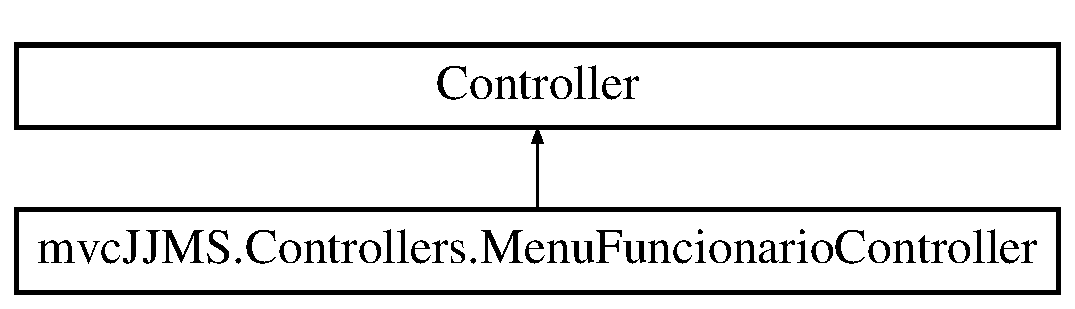
\includegraphics[height=2.000000cm]{classmvc_j_j_m_s_1_1_controllers_1_1_menu_funcionario_controller}
\end{center}
\end{figure}
\subsection*{Public Member Functions}
\begin{DoxyCompactItemize}
\item 
\mbox{\Hypertarget{classmvc_j_j_m_s_1_1_controllers_1_1_menu_funcionario_controller_a1ec34512098549061ef57e7b8ef07945}\label{classmvc_j_j_m_s_1_1_controllers_1_1_menu_funcionario_controller_a1ec34512098549061ef57e7b8ef07945}} 
{\bfseries Menu\+Funcionario\+Controller} (\mbox{\hyperlink{classmvc_j_j_m_s_1_1_data_1_1_j_j_m_s_context}{J\+J\+M\+S\+Context}} context, \mbox{\hyperlink{classmvc_j_j_m_s_1_1_controllers_1_1_encomenda_controller}{Encomenda\+Controller}} e\+Controller, \mbox{\hyperlink{classmvc_j_j_m_s_1_1_controllers_1_1_funcionario_controller}{Funcionario\+Controller}} f\+Controller, \mbox{\hyperlink{classmvc_j_j_m_s_1_1_controllers_1_1_cliente_controller}{Cliente\+Controller}} c\+Controller, \mbox{\hyperlink{classmvc_j_j_m_s_1_1_controllers_1_1_fornecedor_controller}{Fornecedor\+Controller}} forn\+Controller, \mbox{\hyperlink{classmvc_j_j_m_s_1_1_controllers_1_1_utilizador_controller}{Utilizador\+Controller}} u\+Controller)
\item 
View\+Result \mbox{\hyperlink{classmvc_j_j_m_s_1_1_controllers_1_1_menu_funcionario_controller_acdc18ba7b60c90728254ff66cf523c10}{Index}} ()
\begin{DoxyCompactList}\small\item\em Show the menu of Funcionario(employee) \end{DoxyCompactList}\item 
View\+Result \mbox{\hyperlink{classmvc_j_j_m_s_1_1_controllers_1_1_menu_funcionario_controller_aa3969c230e6f472ebe0241d6399e29c9}{Calcular\+Rota}} (string origem, string destino)
\begin{DoxyCompactList}\small\item\em Calculates the route between origem(source) adress and destino(destiny) adress \end{DoxyCompactList}\item 
View\+Result \mbox{\hyperlink{classmvc_j_j_m_s_1_1_controllers_1_1_menu_funcionario_controller_aafa0339ff14c5dfd9bb25a36efa89538}{Calcular\+Rota}} (int id\+Encomenda, string origem)
\begin{DoxyCompactList}\small\item\em Obtain route for an Encomenda(order) where Funcionario(employee) is at origem adress \end{DoxyCompactList}\item 
\mbox{\Hypertarget{classmvc_j_j_m_s_1_1_controllers_1_1_menu_funcionario_controller_a579dc46926cba210b05c6b3dca4061a5}\label{classmvc_j_j_m_s_1_1_controllers_1_1_menu_funcionario_controller_a579dc46926cba210b05c6b3dca4061a5}} 
View\+Result {\bfseries Consultar\+Rota} ()
\item 
Action\+Result \mbox{\hyperlink{classmvc_j_j_m_s_1_1_controllers_1_1_menu_funcionario_controller_a6b3d80d3a3c8ec6cffddf1a21ca6606f}{Consultar\+Rota\+Res}} (string id\+EncS, string origem)
\begin{DoxyCompactList}\small\item\em Allow Funcionario(employee) to consult a route for an Encomenda(order) with id\+EncS, verify if Encomenda(order) is a valid one and if is returns the route \end{DoxyCompactList}\item 
\mbox{\Hypertarget{classmvc_j_j_m_s_1_1_controllers_1_1_menu_funcionario_controller_a79f757c8123a389769358fa4a39011fd}\label{classmvc_j_j_m_s_1_1_controllers_1_1_menu_funcionario_controller_a79f757c8123a389769358fa4a39011fd}} 
View\+Result {\bfseries Encomenda\+Inexistente} ()
\item 
\mbox{\Hypertarget{classmvc_j_j_m_s_1_1_controllers_1_1_menu_funcionario_controller_a2144dac1033881d1b96d2a2f24308104}\label{classmvc_j_j_m_s_1_1_controllers_1_1_menu_funcionario_controller_a2144dac1033881d1b96d2a2f24308104}} 
View\+Result {\bfseries Encomenda\+Invalida} ()
\item 
\mbox{\Hypertarget{classmvc_j_j_m_s_1_1_controllers_1_1_menu_funcionario_controller_a2b03ef8c9cf04a249eced8f43ae34d04}\label{classmvc_j_j_m_s_1_1_controllers_1_1_menu_funcionario_controller_a2b03ef8c9cf04a249eced8f43ae34d04}} 
View\+Result {\bfseries Atualizar\+Estado} ()
\item 
View\+Result \mbox{\hyperlink{classmvc_j_j_m_s_1_1_controllers_1_1_menu_funcionario_controller_ad45a069bdf6baf93b0851b7eef2d9088}{Atualizar\+Estado\+Custo}} (string id\+Encomenda)
\begin{DoxyCompactList}\small\item\em Checks if Encomenda(order) with id\+Encomenda is valid and return the correpondent view \end{DoxyCompactList}\item 
Action\+Result \mbox{\hyperlink{classmvc_j_j_m_s_1_1_controllers_1_1_menu_funcionario_controller_a9eaa1e9f78c031cb0431158442e5f0c2}{Atualizar\+Estado\+Res}} (string id\+Encomenda, string custo\+Input)
\begin{DoxyCompactList}\small\item\em checks cost(custo\+Input) and updates state and total cost of order with id id\+Encomenda, and depending the state delegate a employee or activate the payment of the service \end{DoxyCompactList}\item 
\mbox{\Hypertarget{classmvc_j_j_m_s_1_1_controllers_1_1_menu_funcionario_controller_a0015d1625c1d944fdf5356668e4bf5c3}\label{classmvc_j_j_m_s_1_1_controllers_1_1_menu_funcionario_controller_a0015d1625c1d944fdf5356668e4bf5c3}} 
View\+Result {\bfseries Atualizado\+Com\+Sucesso} ()
\item 
\mbox{\Hypertarget{classmvc_j_j_m_s_1_1_controllers_1_1_menu_funcionario_controller_a8cc1bf95b689ed613164331ac110f54b}\label{classmvc_j_j_m_s_1_1_controllers_1_1_menu_funcionario_controller_a8cc1bf95b689ed613164331ac110f54b}} 
View\+Result {\bfseries Custo\+Invalido} ()
\item 
\mbox{\Hypertarget{classmvc_j_j_m_s_1_1_controllers_1_1_menu_funcionario_controller_ad9a542852b6a8ea1d9535f022c8a1142}\label{classmvc_j_j_m_s_1_1_controllers_1_1_menu_funcionario_controller_ad9a542852b6a8ea1d9535f022c8a1142}} 
View\+Result {\bfseries Nao\+Existe\+Encomenda} ()
\item 
void \mbox{\hyperlink{classmvc_j_j_m_s_1_1_controllers_1_1_menu_funcionario_controller_a28c1cd92d5ef866174d66b5b61b95bc6}{Delegar\+Funcionario}} (int id\+Encomenda)
\begin{DoxyCompactList}\small\item\em Delegates an Funcionario(employee) for the Encomenda(order) with id id\+Encomenda \end{DoxyCompactList}\end{DoxyCompactItemize}


\subsection{Member Function Documentation}
\mbox{\Hypertarget{classmvc_j_j_m_s_1_1_controllers_1_1_menu_funcionario_controller_ad45a069bdf6baf93b0851b7eef2d9088}\label{classmvc_j_j_m_s_1_1_controllers_1_1_menu_funcionario_controller_ad45a069bdf6baf93b0851b7eef2d9088}} 
\index{mvc\+J\+J\+M\+S\+::\+Controllers\+::\+Menu\+Funcionario\+Controller@{mvc\+J\+J\+M\+S\+::\+Controllers\+::\+Menu\+Funcionario\+Controller}!Atualizar\+Estado\+Custo@{Atualizar\+Estado\+Custo}}
\index{Atualizar\+Estado\+Custo@{Atualizar\+Estado\+Custo}!mvc\+J\+J\+M\+S\+::\+Controllers\+::\+Menu\+Funcionario\+Controller@{mvc\+J\+J\+M\+S\+::\+Controllers\+::\+Menu\+Funcionario\+Controller}}
\subsubsection{\texorpdfstring{Atualizar\+Estado\+Custo()}{AtualizarEstadoCusto()}}
{\footnotesize\ttfamily View\+Result mvc\+J\+J\+M\+S.\+Controllers.\+Menu\+Funcionario\+Controller.\+Atualizar\+Estado\+Custo (\begin{DoxyParamCaption}\item[{string}]{id\+Encomenda }\end{DoxyParamCaption})\hspace{0.3cm}{\ttfamily [inline]}}



Checks if Encomenda(order) with id\+Encomenda is valid and return the correpondent view 


\begin{DoxyParams}{Parameters}
{\em id\+Encomenda} & \\
\hline
\end{DoxyParams}
\begin{DoxyReturn}{Returns}
return the correspondent view
\end{DoxyReturn}
\mbox{\Hypertarget{classmvc_j_j_m_s_1_1_controllers_1_1_menu_funcionario_controller_a9eaa1e9f78c031cb0431158442e5f0c2}\label{classmvc_j_j_m_s_1_1_controllers_1_1_menu_funcionario_controller_a9eaa1e9f78c031cb0431158442e5f0c2}} 
\index{mvc\+J\+J\+M\+S\+::\+Controllers\+::\+Menu\+Funcionario\+Controller@{mvc\+J\+J\+M\+S\+::\+Controllers\+::\+Menu\+Funcionario\+Controller}!Atualizar\+Estado\+Res@{Atualizar\+Estado\+Res}}
\index{Atualizar\+Estado\+Res@{Atualizar\+Estado\+Res}!mvc\+J\+J\+M\+S\+::\+Controllers\+::\+Menu\+Funcionario\+Controller@{mvc\+J\+J\+M\+S\+::\+Controllers\+::\+Menu\+Funcionario\+Controller}}
\subsubsection{\texorpdfstring{Atualizar\+Estado\+Res()}{AtualizarEstadoRes()}}
{\footnotesize\ttfamily Action\+Result mvc\+J\+J\+M\+S.\+Controllers.\+Menu\+Funcionario\+Controller.\+Atualizar\+Estado\+Res (\begin{DoxyParamCaption}\item[{string}]{id\+Encomenda,  }\item[{string}]{custo\+Input }\end{DoxyParamCaption})\hspace{0.3cm}{\ttfamily [inline]}}



checks cost(custo\+Input) and updates state and total cost of order with id id\+Encomenda, and depending the state delegate a employee or activate the payment of the service 


\begin{DoxyParams}{Parameters}
{\em id\+Encomenda} & \\
\hline
{\em custo\+Input} & \\
\hline
\end{DoxyParams}
\begin{DoxyReturn}{Returns}
return the correspondent action
\end{DoxyReturn}
\mbox{\Hypertarget{classmvc_j_j_m_s_1_1_controllers_1_1_menu_funcionario_controller_aa3969c230e6f472ebe0241d6399e29c9}\label{classmvc_j_j_m_s_1_1_controllers_1_1_menu_funcionario_controller_aa3969c230e6f472ebe0241d6399e29c9}} 
\index{mvc\+J\+J\+M\+S\+::\+Controllers\+::\+Menu\+Funcionario\+Controller@{mvc\+J\+J\+M\+S\+::\+Controllers\+::\+Menu\+Funcionario\+Controller}!Calcular\+Rota@{Calcular\+Rota}}
\index{Calcular\+Rota@{Calcular\+Rota}!mvc\+J\+J\+M\+S\+::\+Controllers\+::\+Menu\+Funcionario\+Controller@{mvc\+J\+J\+M\+S\+::\+Controllers\+::\+Menu\+Funcionario\+Controller}}
\subsubsection{\texorpdfstring{Calcular\+Rota()}{CalcularRota()}\hspace{0.1cm}{\footnotesize\ttfamily [1/2]}}
{\footnotesize\ttfamily View\+Result mvc\+J\+J\+M\+S.\+Controllers.\+Menu\+Funcionario\+Controller.\+Calcular\+Rota (\begin{DoxyParamCaption}\item[{string}]{origem,  }\item[{string}]{destino }\end{DoxyParamCaption})\hspace{0.3cm}{\ttfamily [inline]}}



Calculates the route between origem(source) adress and destino(destiny) adress 


\begin{DoxyParams}{Parameters}
{\em origem} & \\
\hline
{\em destino} & \\
\hline
\end{DoxyParams}
\begin{DoxyReturn}{Returns}
return route
\end{DoxyReturn}
\mbox{\Hypertarget{classmvc_j_j_m_s_1_1_controllers_1_1_menu_funcionario_controller_aafa0339ff14c5dfd9bb25a36efa89538}\label{classmvc_j_j_m_s_1_1_controllers_1_1_menu_funcionario_controller_aafa0339ff14c5dfd9bb25a36efa89538}} 
\index{mvc\+J\+J\+M\+S\+::\+Controllers\+::\+Menu\+Funcionario\+Controller@{mvc\+J\+J\+M\+S\+::\+Controllers\+::\+Menu\+Funcionario\+Controller}!Calcular\+Rota@{Calcular\+Rota}}
\index{Calcular\+Rota@{Calcular\+Rota}!mvc\+J\+J\+M\+S\+::\+Controllers\+::\+Menu\+Funcionario\+Controller@{mvc\+J\+J\+M\+S\+::\+Controllers\+::\+Menu\+Funcionario\+Controller}}
\subsubsection{\texorpdfstring{Calcular\+Rota()}{CalcularRota()}\hspace{0.1cm}{\footnotesize\ttfamily [2/2]}}
{\footnotesize\ttfamily View\+Result mvc\+J\+J\+M\+S.\+Controllers.\+Menu\+Funcionario\+Controller.\+Calcular\+Rota (\begin{DoxyParamCaption}\item[{int}]{id\+Encomenda,  }\item[{string}]{origem }\end{DoxyParamCaption})\hspace{0.3cm}{\ttfamily [inline]}}



Obtain route for an Encomenda(order) where Funcionario(employee) is at origem adress 


\begin{DoxyParams}{Parameters}
{\em id\+Encomenda} & \\
\hline
{\em origem} & \\
\hline
\end{DoxyParams}
\begin{DoxyReturn}{Returns}
return route
\end{DoxyReturn}
\mbox{\Hypertarget{classmvc_j_j_m_s_1_1_controllers_1_1_menu_funcionario_controller_a6b3d80d3a3c8ec6cffddf1a21ca6606f}\label{classmvc_j_j_m_s_1_1_controllers_1_1_menu_funcionario_controller_a6b3d80d3a3c8ec6cffddf1a21ca6606f}} 
\index{mvc\+J\+J\+M\+S\+::\+Controllers\+::\+Menu\+Funcionario\+Controller@{mvc\+J\+J\+M\+S\+::\+Controllers\+::\+Menu\+Funcionario\+Controller}!Consultar\+Rota\+Res@{Consultar\+Rota\+Res}}
\index{Consultar\+Rota\+Res@{Consultar\+Rota\+Res}!mvc\+J\+J\+M\+S\+::\+Controllers\+::\+Menu\+Funcionario\+Controller@{mvc\+J\+J\+M\+S\+::\+Controllers\+::\+Menu\+Funcionario\+Controller}}
\subsubsection{\texorpdfstring{Consultar\+Rota\+Res()}{ConsultarRotaRes()}}
{\footnotesize\ttfamily Action\+Result mvc\+J\+J\+M\+S.\+Controllers.\+Menu\+Funcionario\+Controller.\+Consultar\+Rota\+Res (\begin{DoxyParamCaption}\item[{string}]{id\+EncS,  }\item[{string}]{origem }\end{DoxyParamCaption})\hspace{0.3cm}{\ttfamily [inline]}}



Allow Funcionario(employee) to consult a route for an Encomenda(order) with id\+EncS, verify if Encomenda(order) is a valid one and if is returns the route 


\begin{DoxyParams}{Parameters}
{\em id\+EncS} & \\
\hline
{\em origem} & \\
\hline
\end{DoxyParams}
\begin{DoxyReturn}{Returns}
return route
\end{DoxyReturn}
\mbox{\Hypertarget{classmvc_j_j_m_s_1_1_controllers_1_1_menu_funcionario_controller_a28c1cd92d5ef866174d66b5b61b95bc6}\label{classmvc_j_j_m_s_1_1_controllers_1_1_menu_funcionario_controller_a28c1cd92d5ef866174d66b5b61b95bc6}} 
\index{mvc\+J\+J\+M\+S\+::\+Controllers\+::\+Menu\+Funcionario\+Controller@{mvc\+J\+J\+M\+S\+::\+Controllers\+::\+Menu\+Funcionario\+Controller}!Delegar\+Funcionario@{Delegar\+Funcionario}}
\index{Delegar\+Funcionario@{Delegar\+Funcionario}!mvc\+J\+J\+M\+S\+::\+Controllers\+::\+Menu\+Funcionario\+Controller@{mvc\+J\+J\+M\+S\+::\+Controllers\+::\+Menu\+Funcionario\+Controller}}
\subsubsection{\texorpdfstring{Delegar\+Funcionario()}{DelegarFuncionario()}}
{\footnotesize\ttfamily void mvc\+J\+J\+M\+S.\+Controllers.\+Menu\+Funcionario\+Controller.\+Delegar\+Funcionario (\begin{DoxyParamCaption}\item[{int}]{id\+Encomenda }\end{DoxyParamCaption})\hspace{0.3cm}{\ttfamily [inline]}}



Delegates an Funcionario(employee) for the Encomenda(order) with id id\+Encomenda 


\begin{DoxyParams}{Parameters}
{\em id\+Encomenda} & \\
\hline
\end{DoxyParams}
\mbox{\Hypertarget{classmvc_j_j_m_s_1_1_controllers_1_1_menu_funcionario_controller_acdc18ba7b60c90728254ff66cf523c10}\label{classmvc_j_j_m_s_1_1_controllers_1_1_menu_funcionario_controller_acdc18ba7b60c90728254ff66cf523c10}} 
\index{mvc\+J\+J\+M\+S\+::\+Controllers\+::\+Menu\+Funcionario\+Controller@{mvc\+J\+J\+M\+S\+::\+Controllers\+::\+Menu\+Funcionario\+Controller}!Index@{Index}}
\index{Index@{Index}!mvc\+J\+J\+M\+S\+::\+Controllers\+::\+Menu\+Funcionario\+Controller@{mvc\+J\+J\+M\+S\+::\+Controllers\+::\+Menu\+Funcionario\+Controller}}
\subsubsection{\texorpdfstring{Index()}{Index()}}
{\footnotesize\ttfamily View\+Result mvc\+J\+J\+M\+S.\+Controllers.\+Menu\+Funcionario\+Controller.\+Index (\begin{DoxyParamCaption}{ }\end{DoxyParamCaption})\hspace{0.3cm}{\ttfamily [inline]}}



Show the menu of Funcionario(employee) 

\begin{DoxyReturn}{Returns}
Menu\+Funcionario
\end{DoxyReturn}


The documentation for this class was generated from the following file\+:\begin{DoxyCompactItemize}
\item 
Controllers/Menu\+Funcionario\+Controller.\+cs\end{DoxyCompactItemize}

\hypertarget{classmvc_j_j_m_s_1_1_controllers_1_1_menu_principal_controller}{}\section{mvc\+J\+J\+M\+S.\+Controllers.\+Menu\+Principal\+Controller Class Reference}
\label{classmvc_j_j_m_s_1_1_controllers_1_1_menu_principal_controller}\index{mvc\+J\+J\+M\+S.\+Controllers.\+Menu\+Principal\+Controller@{mvc\+J\+J\+M\+S.\+Controllers.\+Menu\+Principal\+Controller}}
Inheritance diagram for mvc\+J\+J\+M\+S.\+Controllers.\+Menu\+Principal\+Controller\+:\begin{figure}[H]
\begin{center}
\leavevmode
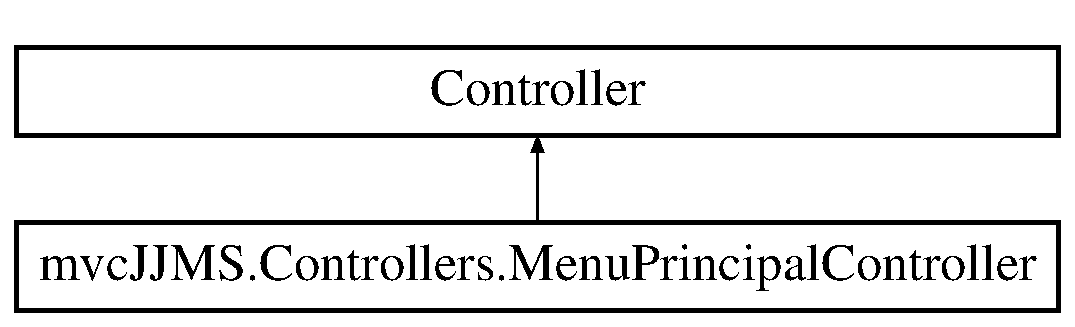
\includegraphics[height=2.000000cm]{classmvc_j_j_m_s_1_1_controllers_1_1_menu_principal_controller}
\end{center}
\end{figure}
\subsection*{Public Member Functions}
\begin{DoxyCompactItemize}
\item 
\mbox{\Hypertarget{classmvc_j_j_m_s_1_1_controllers_1_1_menu_principal_controller_a0e17d9e86a0a271c794b05910ab17af8}\label{classmvc_j_j_m_s_1_1_controllers_1_1_menu_principal_controller_a0e17d9e86a0a271c794b05910ab17af8}} 
View\+Result {\bfseries Index} ()
\item 
View\+Result \mbox{\hyperlink{classmvc_j_j_m_s_1_1_controllers_1_1_menu_principal_controller_aaa09d4cb83794cb17bdb5f9c7dffdd3d}{Login}} ()
\begin{DoxyCompactList}\small\item\em Wrapper for the \mbox{\hyperlink{classmvc_j_j_m_s_1_1_controllers_1_1_utilizador_controller_af8335bb74fe7e7b4cbab85a176775c30}{Utilizador\+Controller.\+Login}} method \end{DoxyCompactList}\item 
View\+Result \mbox{\hyperlink{classmvc_j_j_m_s_1_1_controllers_1_1_menu_principal_controller_a3ca7f041e21c6d3c633e255d96785d52}{Registar}} ()
\begin{DoxyCompactList}\small\item\em Wrapper for the \mbox{\hyperlink{classmvc_j_j_m_s_1_1_controllers_1_1_cliente_controller_a31325ea0231ffa6f09996a9f61f1731b}{Cliente\+Controller.\+Registar}} method \end{DoxyCompactList}\end{DoxyCompactItemize}


\subsection{Member Function Documentation}
\mbox{\Hypertarget{classmvc_j_j_m_s_1_1_controllers_1_1_menu_principal_controller_aaa09d4cb83794cb17bdb5f9c7dffdd3d}\label{classmvc_j_j_m_s_1_1_controllers_1_1_menu_principal_controller_aaa09d4cb83794cb17bdb5f9c7dffdd3d}} 
\index{mvc\+J\+J\+M\+S\+::\+Controllers\+::\+Menu\+Principal\+Controller@{mvc\+J\+J\+M\+S\+::\+Controllers\+::\+Menu\+Principal\+Controller}!Login@{Login}}
\index{Login@{Login}!mvc\+J\+J\+M\+S\+::\+Controllers\+::\+Menu\+Principal\+Controller@{mvc\+J\+J\+M\+S\+::\+Controllers\+::\+Menu\+Principal\+Controller}}
\subsubsection{\texorpdfstring{Login()}{Login()}}
{\footnotesize\ttfamily View\+Result mvc\+J\+J\+M\+S.\+Controllers.\+Menu\+Principal\+Controller.\+Login (\begin{DoxyParamCaption}{ }\end{DoxyParamCaption})\hspace{0.3cm}{\ttfamily [inline]}}



Wrapper for the \mbox{\hyperlink{classmvc_j_j_m_s_1_1_controllers_1_1_utilizador_controller_af8335bb74fe7e7b4cbab85a176775c30}{Utilizador\+Controller.\+Login}} method 

\begin{DoxyReturn}{Returns}
View of the login page
\end{DoxyReturn}
\mbox{\Hypertarget{classmvc_j_j_m_s_1_1_controllers_1_1_menu_principal_controller_a3ca7f041e21c6d3c633e255d96785d52}\label{classmvc_j_j_m_s_1_1_controllers_1_1_menu_principal_controller_a3ca7f041e21c6d3c633e255d96785d52}} 
\index{mvc\+J\+J\+M\+S\+::\+Controllers\+::\+Menu\+Principal\+Controller@{mvc\+J\+J\+M\+S\+::\+Controllers\+::\+Menu\+Principal\+Controller}!Registar@{Registar}}
\index{Registar@{Registar}!mvc\+J\+J\+M\+S\+::\+Controllers\+::\+Menu\+Principal\+Controller@{mvc\+J\+J\+M\+S\+::\+Controllers\+::\+Menu\+Principal\+Controller}}
\subsubsection{\texorpdfstring{Registar()}{Registar()}}
{\footnotesize\ttfamily View\+Result mvc\+J\+J\+M\+S.\+Controllers.\+Menu\+Principal\+Controller.\+Registar (\begin{DoxyParamCaption}{ }\end{DoxyParamCaption})\hspace{0.3cm}{\ttfamily [inline]}}



Wrapper for the \mbox{\hyperlink{classmvc_j_j_m_s_1_1_controllers_1_1_cliente_controller_a31325ea0231ffa6f09996a9f61f1731b}{Cliente\+Controller.\+Registar}} method 

\begin{DoxyReturn}{Returns}
View of the registration page
\end{DoxyReturn}


The documentation for this class was generated from the following file\+:\begin{DoxyCompactItemize}
\item 
Controllers/Menu\+Principal\+Controller.\+cs\end{DoxyCompactItemize}

\hypertarget{classmvc_j_j_m_s_1_1_models_1_1_utilizador}{}\section{mvc\+J\+J\+M\+S.\+Models.\+Utilizador Class Reference}
\label{classmvc_j_j_m_s_1_1_models_1_1_utilizador}\index{mvc\+J\+J\+M\+S.\+Models.\+Utilizador@{mvc\+J\+J\+M\+S.\+Models.\+Utilizador}}


Represents a single user whether a Client or an Employee  


Inheritance diagram for mvc\+J\+J\+M\+S.\+Models.\+Utilizador\+:\begin{figure}[H]
\begin{center}
\leavevmode
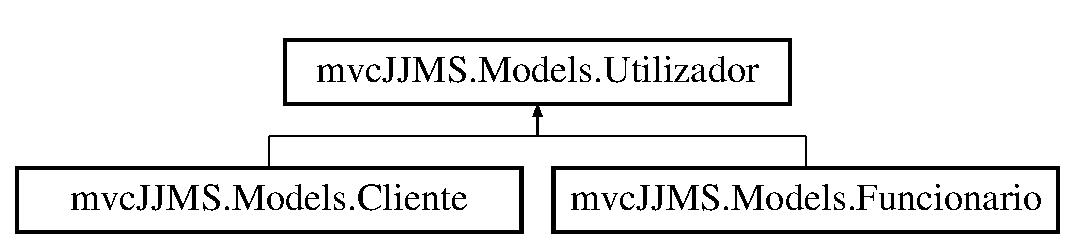
\includegraphics[height=2.000000cm]{classmvc_j_j_m_s_1_1_models_1_1_utilizador}
\end{center}
\end{figure}
\subsection*{Properties}
\begin{DoxyCompactItemize}
\item 
\mbox{\Hypertarget{classmvc_j_j_m_s_1_1_models_1_1_utilizador_a35562436f48a986eaa6e3ce1dc350718}\label{classmvc_j_j_m_s_1_1_models_1_1_utilizador_a35562436f48a986eaa6e3ce1dc350718}} 
int {\bfseries Utilizador\+ID}\hspace{0.3cm}{\ttfamily  \mbox{[}get, set\mbox{]}}
\item 
\mbox{\Hypertarget{classmvc_j_j_m_s_1_1_models_1_1_utilizador_a84b2d5179fb51a1722818126cd1902c4}\label{classmvc_j_j_m_s_1_1_models_1_1_utilizador_a84b2d5179fb51a1722818126cd1902c4}} 
string {\bfseries Email}\hspace{0.3cm}{\ttfamily  \mbox{[}get, set\mbox{]}}
\item 
\mbox{\Hypertarget{classmvc_j_j_m_s_1_1_models_1_1_utilizador_a4cb4c440341216f629aef41e3f078560}\label{classmvc_j_j_m_s_1_1_models_1_1_utilizador_a4cb4c440341216f629aef41e3f078560}} 
byte \mbox{[}$\,$\mbox{]} {\bfseries Password}\hspace{0.3cm}{\ttfamily  \mbox{[}get, set\mbox{]}}
\item 
\mbox{\Hypertarget{classmvc_j_j_m_s_1_1_models_1_1_utilizador_a6f09601a2135efaf2d5ae2a3761791cb}\label{classmvc_j_j_m_s_1_1_models_1_1_utilizador_a6f09601a2135efaf2d5ae2a3761791cb}} 
string {\bfseries Nome}\hspace{0.3cm}{\ttfamily  \mbox{[}get, set\mbox{]}}
\end{DoxyCompactItemize}


\subsection{Detailed Description}
Represents a single user whether a Client or an Employee 



The documentation for this class was generated from the following file\+:\begin{DoxyCompactItemize}
\item 
Models/Utilizador.\+cs\end{DoxyCompactItemize}

\hypertarget{classmvc_j_j_m_s_1_1_controllers_1_1_utilizador_controller}{}\section{mvc\+J\+J\+M\+S.\+Controllers.\+Utilizador\+Controller Class Reference}
\label{classmvc_j_j_m_s_1_1_controllers_1_1_utilizador_controller}\index{mvc\+J\+J\+M\+S.\+Controllers.\+Utilizador\+Controller@{mvc\+J\+J\+M\+S.\+Controllers.\+Utilizador\+Controller}}
Inheritance diagram for mvc\+J\+J\+M\+S.\+Controllers.\+Utilizador\+Controller\+:\begin{figure}[H]
\begin{center}
\leavevmode
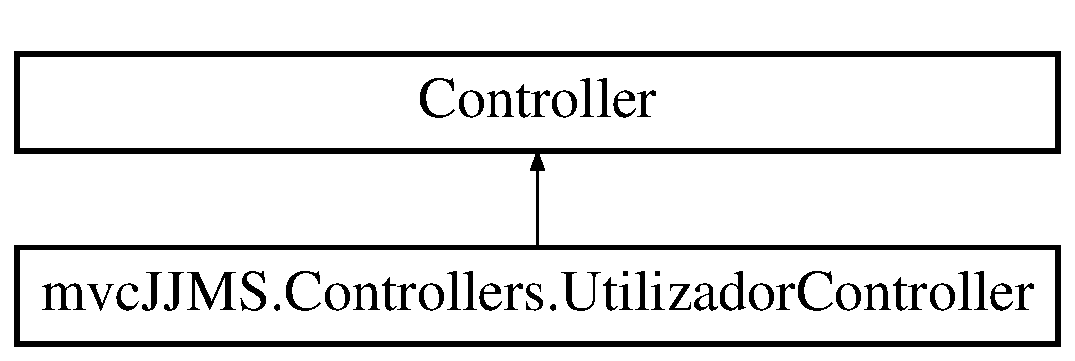
\includegraphics[height=2.000000cm]{classmvc_j_j_m_s_1_1_controllers_1_1_utilizador_controller}
\end{center}
\end{figure}
\subsection*{Public Member Functions}
\begin{DoxyCompactItemize}
\item 
\mbox{\Hypertarget{classmvc_j_j_m_s_1_1_controllers_1_1_utilizador_controller_a1d833224478b16de3a404928df7c6fb0}\label{classmvc_j_j_m_s_1_1_controllers_1_1_utilizador_controller_a1d833224478b16de3a404928df7c6fb0}} 
{\bfseries Utilizador\+Controller} (\mbox{\hyperlink{classmvc_j_j_m_s_1_1_data_1_1_j_j_m_s_context}{J\+J\+M\+S\+Context}} context)
\item 
Action\+Result \mbox{\hyperlink{classmvc_j_j_m_s_1_1_controllers_1_1_utilizador_controller_af8335bb74fe7e7b4cbab85a176775c30}{Login}} (string email, string password)
\begin{DoxyCompactList}\small\item\em Logs a user into the system \end{DoxyCompactList}\item 
int \mbox{\hyperlink{classmvc_j_j_m_s_1_1_controllers_1_1_utilizador_controller_a8243cd298846e34fb97c3c7d2d691174}{get\+Utilizador\+ID}} ()
\begin{DoxyCompactList}\small\item\em Returns the ID of the user currently logged in \end{DoxyCompactList}\item 
bool \mbox{\hyperlink{classmvc_j_j_m_s_1_1_controllers_1_1_utilizador_controller_abc0b8e9e7e35ee0c6f910a4fc63bb6d2}{email\+Associado}} (string email)
\begin{DoxyCompactList}\small\item\em Checks whether there\textquotesingle{}s a registered user with the given email \end{DoxyCompactList}\item 
string \mbox{\hyperlink{classmvc_j_j_m_s_1_1_controllers_1_1_utilizador_controller_a6250c090d89e8a6cea8347d9186daeb0}{Get\+User\+Nome}} (int id\+User)
\begin{DoxyCompactList}\small\item\em Retrieves the username associated with the given user ID \end{DoxyCompactList}\item 
byte \mbox{[}$\,$\mbox{]} \mbox{\hyperlink{classmvc_j_j_m_s_1_1_controllers_1_1_utilizador_controller_a71ba7901a09e013703d461927ab9ff80}{Get\+User\+Password}} (int id\+User)
\begin{DoxyCompactList}\small\item\em Retrieves the password associated with the given user ID \end{DoxyCompactList}\item 
string \mbox{\hyperlink{classmvc_j_j_m_s_1_1_controllers_1_1_utilizador_controller_a11bcddd35c8eeaaea9a7baf761b8f877}{Get\+User\+Email}} (int id\+User)
\begin{DoxyCompactList}\small\item\em Retrieves the email associated with the given user ID \end{DoxyCompactList}\item 
void \mbox{\hyperlink{classmvc_j_j_m_s_1_1_controllers_1_1_utilizador_controller_ae6ce52cd52288d470fb4d57da79dbffb}{Update\+Nome}} (int id\+User, string nome\+Input)
\begin{DoxyCompactList}\small\item\em Updates the username associated with the given user ID \end{DoxyCompactList}\item 
void \mbox{\hyperlink{classmvc_j_j_m_s_1_1_controllers_1_1_utilizador_controller_a9dec9a63e5d6e07567c884db33e69ef3}{Update\+Password}} (int id\+User, string password\+Input)
\begin{DoxyCompactList}\small\item\em Updates the password associated with the given user ID \end{DoxyCompactList}\item 
void \mbox{\hyperlink{classmvc_j_j_m_s_1_1_controllers_1_1_utilizador_controller_a11aabb148f5c11805d2fc9955a44a91d}{Update\+Email}} (int id\+User, string email\+Input)
\begin{DoxyCompactList}\small\item\em Updates the email associated with the given user ID \end{DoxyCompactList}\item 
\mbox{\Hypertarget{classmvc_j_j_m_s_1_1_controllers_1_1_utilizador_controller_a2be8952c2ef886358ba107f962199a00}\label{classmvc_j_j_m_s_1_1_controllers_1_1_utilizador_controller_a2be8952c2ef886358ba107f962199a00}} 
View\+Result {\bfseries Email\+Inexistente} ()
\item 
\mbox{\Hypertarget{classmvc_j_j_m_s_1_1_controllers_1_1_utilizador_controller_ac0481a2c0ce4068349866c229abaa9eb}\label{classmvc_j_j_m_s_1_1_controllers_1_1_utilizador_controller_ac0481a2c0ce4068349866c229abaa9eb}} 
View\+Result {\bfseries Password\+Invalida} ()
\end{DoxyCompactItemize}
\subsection*{Static Public Member Functions}
\begin{DoxyCompactItemize}
\item 
static byte \mbox{[}$\,$\mbox{]} \mbox{\hyperlink{classmvc_j_j_m_s_1_1_controllers_1_1_utilizador_controller_a72e105c651070200f84c3718fdf3c8cc}{ hash\+Function}} (string input)
\begin{DoxyCompactList}\small\item\em Performas a sha384 hash on the input string \end{DoxyCompactList}\end{DoxyCompactItemize}


\subsection{Member Function Documentation}
\mbox{\Hypertarget{classmvc_j_j_m_s_1_1_controllers_1_1_utilizador_controller_abc0b8e9e7e35ee0c6f910a4fc63bb6d2}\label{classmvc_j_j_m_s_1_1_controllers_1_1_utilizador_controller_abc0b8e9e7e35ee0c6f910a4fc63bb6d2}} 
\index{mvc\+J\+J\+M\+S\+::\+Controllers\+::\+Utilizador\+Controller@{mvc\+J\+J\+M\+S\+::\+Controllers\+::\+Utilizador\+Controller}!email\+Associado@{email\+Associado}}
\index{email\+Associado@{email\+Associado}!mvc\+J\+J\+M\+S\+::\+Controllers\+::\+Utilizador\+Controller@{mvc\+J\+J\+M\+S\+::\+Controllers\+::\+Utilizador\+Controller}}
\subsubsection{\texorpdfstring{email\+Associado()}{emailAssociado()}}
{\footnotesize\ttfamily bool mvc\+J\+J\+M\+S.\+Controllers.\+Utilizador\+Controller.\+email\+Associado (\begin{DoxyParamCaption}\item[{string}]{email }\end{DoxyParamCaption})\hspace{0.3cm}{\ttfamily [inline]}}



Checks whether there\textquotesingle{}s a registered user with the given email 


\begin{DoxyParams}{Parameters}
{\em email} & Email address to check for\\
\hline
\end{DoxyParams}
\begin{DoxyReturn}{Returns}
T\+R\+UE if there is a user registered with the email else F\+A\+L\+SE
\end{DoxyReturn}
\mbox{\Hypertarget{classmvc_j_j_m_s_1_1_controllers_1_1_utilizador_controller_a11bcddd35c8eeaaea9a7baf761b8f877}\label{classmvc_j_j_m_s_1_1_controllers_1_1_utilizador_controller_a11bcddd35c8eeaaea9a7baf761b8f877}} 
\index{mvc\+J\+J\+M\+S\+::\+Controllers\+::\+Utilizador\+Controller@{mvc\+J\+J\+M\+S\+::\+Controllers\+::\+Utilizador\+Controller}!Get\+User\+Email@{Get\+User\+Email}}
\index{Get\+User\+Email@{Get\+User\+Email}!mvc\+J\+J\+M\+S\+::\+Controllers\+::\+Utilizador\+Controller@{mvc\+J\+J\+M\+S\+::\+Controllers\+::\+Utilizador\+Controller}}
\subsubsection{\texorpdfstring{Get\+User\+Email()}{GetUserEmail()}}
{\footnotesize\ttfamily string mvc\+J\+J\+M\+S.\+Controllers.\+Utilizador\+Controller.\+Get\+User\+Email (\begin{DoxyParamCaption}\item[{int}]{id\+User }\end{DoxyParamCaption})\hspace{0.3cm}{\ttfamily [inline]}}



Retrieves the email associated with the given user ID 


\begin{DoxyParams}{Parameters}
{\em id\+User} & Unique identifier of the user\\
\hline
\end{DoxyParams}
\begin{DoxyReturn}{Returns}
Email associated with the identifier
\end{DoxyReturn}
\mbox{\Hypertarget{classmvc_j_j_m_s_1_1_controllers_1_1_utilizador_controller_a6250c090d89e8a6cea8347d9186daeb0}\label{classmvc_j_j_m_s_1_1_controllers_1_1_utilizador_controller_a6250c090d89e8a6cea8347d9186daeb0}} 
\index{mvc\+J\+J\+M\+S\+::\+Controllers\+::\+Utilizador\+Controller@{mvc\+J\+J\+M\+S\+::\+Controllers\+::\+Utilizador\+Controller}!Get\+User\+Nome@{Get\+User\+Nome}}
\index{Get\+User\+Nome@{Get\+User\+Nome}!mvc\+J\+J\+M\+S\+::\+Controllers\+::\+Utilizador\+Controller@{mvc\+J\+J\+M\+S\+::\+Controllers\+::\+Utilizador\+Controller}}
\subsubsection{\texorpdfstring{Get\+User\+Nome()}{GetUserNome()}}
{\footnotesize\ttfamily string mvc\+J\+J\+M\+S.\+Controllers.\+Utilizador\+Controller.\+Get\+User\+Nome (\begin{DoxyParamCaption}\item[{int}]{id\+User }\end{DoxyParamCaption})\hspace{0.3cm}{\ttfamily [inline]}}



Retrieves the username associated with the given user ID 


\begin{DoxyParams}{Parameters}
{\em id\+User} & Unique identifier of the user\\
\hline
\end{DoxyParams}
\begin{DoxyReturn}{Returns}
Username associated with the identifier
\end{DoxyReturn}
\mbox{\Hypertarget{classmvc_j_j_m_s_1_1_controllers_1_1_utilizador_controller_a71ba7901a09e013703d461927ab9ff80}\label{classmvc_j_j_m_s_1_1_controllers_1_1_utilizador_controller_a71ba7901a09e013703d461927ab9ff80}} 
\index{mvc\+J\+J\+M\+S\+::\+Controllers\+::\+Utilizador\+Controller@{mvc\+J\+J\+M\+S\+::\+Controllers\+::\+Utilizador\+Controller}!Get\+User\+Password@{Get\+User\+Password}}
\index{Get\+User\+Password@{Get\+User\+Password}!mvc\+J\+J\+M\+S\+::\+Controllers\+::\+Utilizador\+Controller@{mvc\+J\+J\+M\+S\+::\+Controllers\+::\+Utilizador\+Controller}}
\subsubsection{\texorpdfstring{Get\+User\+Password()}{GetUserPassword()}}
{\footnotesize\ttfamily byte \mbox{[}$\,$\mbox{]} mvc\+J\+J\+M\+S.\+Controllers.\+Utilizador\+Controller.\+Get\+User\+Password (\begin{DoxyParamCaption}\item[{int}]{id\+User }\end{DoxyParamCaption})\hspace{0.3cm}{\ttfamily [inline]}}



Retrieves the password associated with the given user ID 


\begin{DoxyParams}{Parameters}
{\em id\+User} & Unique identifier of the user\\
\hline
\end{DoxyParams}
\begin{DoxyReturn}{Returns}
Hashed byte array of user password
\end{DoxyReturn}
\mbox{\Hypertarget{classmvc_j_j_m_s_1_1_controllers_1_1_utilizador_controller_a8243cd298846e34fb97c3c7d2d691174}\label{classmvc_j_j_m_s_1_1_controllers_1_1_utilizador_controller_a8243cd298846e34fb97c3c7d2d691174}} 
\index{mvc\+J\+J\+M\+S\+::\+Controllers\+::\+Utilizador\+Controller@{mvc\+J\+J\+M\+S\+::\+Controllers\+::\+Utilizador\+Controller}!get\+Utilizador\+ID@{get\+Utilizador\+ID}}
\index{get\+Utilizador\+ID@{get\+Utilizador\+ID}!mvc\+J\+J\+M\+S\+::\+Controllers\+::\+Utilizador\+Controller@{mvc\+J\+J\+M\+S\+::\+Controllers\+::\+Utilizador\+Controller}}
\subsubsection{\texorpdfstring{get\+Utilizador\+I\+D()}{getUtilizadorID()}}
{\footnotesize\ttfamily int mvc\+J\+J\+M\+S.\+Controllers.\+Utilizador\+Controller.\+get\+Utilizador\+ID (\begin{DoxyParamCaption}{ }\end{DoxyParamCaption})\hspace{0.3cm}{\ttfamily [inline]}}



Returns the ID of the user currently logged in 

\begin{DoxyReturn}{Returns}
Unique identifier of the user
\end{DoxyReturn}
\mbox{\Hypertarget{classmvc_j_j_m_s_1_1_controllers_1_1_utilizador_controller_af8335bb74fe7e7b4cbab85a176775c30}\label{classmvc_j_j_m_s_1_1_controllers_1_1_utilizador_controller_af8335bb74fe7e7b4cbab85a176775c30}} 
\index{mvc\+J\+J\+M\+S\+::\+Controllers\+::\+Utilizador\+Controller@{mvc\+J\+J\+M\+S\+::\+Controllers\+::\+Utilizador\+Controller}!Login@{Login}}
\index{Login@{Login}!mvc\+J\+J\+M\+S\+::\+Controllers\+::\+Utilizador\+Controller@{mvc\+J\+J\+M\+S\+::\+Controllers\+::\+Utilizador\+Controller}}
\subsubsection{\texorpdfstring{Login()}{Login()}}
{\footnotesize\ttfamily Action\+Result mvc\+J\+J\+M\+S.\+Controllers.\+Utilizador\+Controller.\+Login (\begin{DoxyParamCaption}\item[{string}]{email,  }\item[{string}]{password }\end{DoxyParamCaption})\hspace{0.3cm}{\ttfamily [inline]}}



Logs a user into the system 


\begin{DoxyParams}{Parameters}
{\em email} & User email\\
\hline
{\em password} & User password\\
\hline
\end{DoxyParams}
\begin{DoxyReturn}{Returns}
Redirects to a Menu or an Error view
\end{DoxyReturn}
\mbox{\Hypertarget{classmvc_j_j_m_s_1_1_controllers_1_1_utilizador_controller_a11aabb148f5c11805d2fc9955a44a91d}\label{classmvc_j_j_m_s_1_1_controllers_1_1_utilizador_controller_a11aabb148f5c11805d2fc9955a44a91d}} 
\index{mvc\+J\+J\+M\+S\+::\+Controllers\+::\+Utilizador\+Controller@{mvc\+J\+J\+M\+S\+::\+Controllers\+::\+Utilizador\+Controller}!Update\+Email@{Update\+Email}}
\index{Update\+Email@{Update\+Email}!mvc\+J\+J\+M\+S\+::\+Controllers\+::\+Utilizador\+Controller@{mvc\+J\+J\+M\+S\+::\+Controllers\+::\+Utilizador\+Controller}}
\subsubsection{\texorpdfstring{Update\+Email()}{UpdateEmail()}}
{\footnotesize\ttfamily void mvc\+J\+J\+M\+S.\+Controllers.\+Utilizador\+Controller.\+Update\+Email (\begin{DoxyParamCaption}\item[{int}]{id\+User,  }\item[{string}]{email\+Input }\end{DoxyParamCaption})\hspace{0.3cm}{\ttfamily [inline]}}



Updates the email associated with the given user ID 


\begin{DoxyParams}{Parameters}
{\em id\+User} & Unique identifier of the user\\
\hline
{\em email\+Input} & New email\\
\hline
\end{DoxyParams}
\mbox{\Hypertarget{classmvc_j_j_m_s_1_1_controllers_1_1_utilizador_controller_ae6ce52cd52288d470fb4d57da79dbffb}\label{classmvc_j_j_m_s_1_1_controllers_1_1_utilizador_controller_ae6ce52cd52288d470fb4d57da79dbffb}} 
\index{mvc\+J\+J\+M\+S\+::\+Controllers\+::\+Utilizador\+Controller@{mvc\+J\+J\+M\+S\+::\+Controllers\+::\+Utilizador\+Controller}!Update\+Nome@{Update\+Nome}}
\index{Update\+Nome@{Update\+Nome}!mvc\+J\+J\+M\+S\+::\+Controllers\+::\+Utilizador\+Controller@{mvc\+J\+J\+M\+S\+::\+Controllers\+::\+Utilizador\+Controller}}
\subsubsection{\texorpdfstring{Update\+Nome()}{UpdateNome()}}
{\footnotesize\ttfamily void mvc\+J\+J\+M\+S.\+Controllers.\+Utilizador\+Controller.\+Update\+Nome (\begin{DoxyParamCaption}\item[{int}]{id\+User,  }\item[{string}]{nome\+Input }\end{DoxyParamCaption})\hspace{0.3cm}{\ttfamily [inline]}}



Updates the username associated with the given user ID 


\begin{DoxyParams}{Parameters}
{\em id\+User} & Unique identifier of the user\\
\hline
{\em nome\+Input} & New username\\
\hline
\end{DoxyParams}
\mbox{\Hypertarget{classmvc_j_j_m_s_1_1_controllers_1_1_utilizador_controller_a9dec9a63e5d6e07567c884db33e69ef3}\label{classmvc_j_j_m_s_1_1_controllers_1_1_utilizador_controller_a9dec9a63e5d6e07567c884db33e69ef3}} 
\index{mvc\+J\+J\+M\+S\+::\+Controllers\+::\+Utilizador\+Controller@{mvc\+J\+J\+M\+S\+::\+Controllers\+::\+Utilizador\+Controller}!Update\+Password@{Update\+Password}}
\index{Update\+Password@{Update\+Password}!mvc\+J\+J\+M\+S\+::\+Controllers\+::\+Utilizador\+Controller@{mvc\+J\+J\+M\+S\+::\+Controllers\+::\+Utilizador\+Controller}}
\subsubsection{\texorpdfstring{Update\+Password()}{UpdatePassword()}}
{\footnotesize\ttfamily void mvc\+J\+J\+M\+S.\+Controllers.\+Utilizador\+Controller.\+Update\+Password (\begin{DoxyParamCaption}\item[{int}]{id\+User,  }\item[{string}]{password\+Input }\end{DoxyParamCaption})\hspace{0.3cm}{\ttfamily [inline]}}



Updates the password associated with the given user ID 


\begin{DoxyParams}{Parameters}
{\em id\+User} & Unique identifier of the user\\
\hline
{\em password\+Input} & New password\\
\hline
\end{DoxyParams}
\mbox{\Hypertarget{classmvc_j_j_m_s_1_1_controllers_1_1_utilizador_controller_a72e105c651070200f84c3718fdf3c8cc}\label{classmvc_j_j_m_s_1_1_controllers_1_1_utilizador_controller_a72e105c651070200f84c3718fdf3c8cc}} 
\index{mvc\+J\+J\+M\+S\+::\+Controllers\+::\+Utilizador\+Controller@{mvc\+J\+J\+M\+S\+::\+Controllers\+::\+Utilizador\+Controller}! hash\+Function@{ hash\+Function}}
\index{ hash\+Function@{ hash\+Function}!mvc\+J\+J\+M\+S\+::\+Controllers\+::\+Utilizador\+Controller@{mvc\+J\+J\+M\+S\+::\+Controllers\+::\+Utilizador\+Controller}}
\subsubsection{\texorpdfstring{ hash\+Function()}{ hashFunction()}}
{\footnotesize\ttfamily static byte \mbox{[}$\,$\mbox{]} mvc\+J\+J\+M\+S.\+Controllers.\+Utilizador\+Controller.\+ hash\+Function (\begin{DoxyParamCaption}\item[{string}]{input }\end{DoxyParamCaption})\hspace{0.3cm}{\ttfamily [inline]}, {\ttfamily [static]}}



Performas a sha384 hash on the input string 


\begin{DoxyParams}{Parameters}
{\em input} & String to perform the hash on\\
\hline
\end{DoxyParams}
\begin{DoxyReturn}{Returns}
S\+H\+A384 hash output
\end{DoxyReturn}


The documentation for this class was generated from the following file\+:\begin{DoxyCompactItemize}
\item 
Controllers/Utilizador\+Controller.\+cs\end{DoxyCompactItemize}

%--- End generated contents ---

% Index
\backmatter
\newpage
\phantomsection
\clearemptydoublepage
\addcontentsline{toc}{chapter}{Index}
\printindex

\end{document}
